\documentclass[twoside,titlepage]{report}


\usepackage{microtype,amssymb,amsmath,amsfonts,amsthm,fancyhdr,graphicx}
\usepackage{ipad}

%\usepackage{showkeys} %%% This package will show you your labels
                       %%% and should be commented out for the 
                       %%% final print out.
\usepackage{makeidx} %%% gives us our groovy index
%\usepackage[noDcommand]{kpfonts}

\makeindex

%\usepackage{layout} %%% Use command \layout in document to see margins
%%% Use package mathpazo to get another font

%%% These margins are set for 10 pt font size. 
%%% while some may find them to be too large, they 
%%% are set so that no more than 72 characters will
%%% be on any line.  This will help the readability 
%%% of the document.  If the font size is ever increased
%%% then the margins should be increased a bit too.
\oddsidemargin 62pt
\evensidemargin 62pt
\textwidth 345pt
\headheight 14pt




%%% Header and Footer Options
\renewcommand{\headrulewidth}{0.0pt} %%% this takes out the line 
%%%
%\rhead[]{\textsl{\leftmark}}  %%%
%\rfoot[]{\thepage}            %%% Options for 2 sided documents
%\lhead[\textsl{\rightmark}]{} %%%
%\lfoot[\thepage]{}            %%%
%%%
\lhead[\textsl{\rightmark}]{\textsl{\leftmark}} %%% Options for 1 sided documents
\cfoot[]{}                      %%% With typing on the *left* page
\rhead[]{}                                      %%% 
%%%
\cfoot[\thepage]{\thepage} %%% needed for both types of documents
%%% End Header and Footer Options


%%% This sets how the enumerate command works
\renewcommand{\theenumi}{$(\mathrm{\arabic{enumi}})$}
\renewcommand{\labelenumi}{\theenumi}

%%% This next bit of code defines all our theorem environments
\newtheoremstyle{SlantTheorem}{\topsep}{\topsep}%%% space between body and thm
		{\slshape}                      %%% Thm body font
		{}                              %%% Indent amount (empty = no indent)
		{\bfseries\sffamily}            %%% Thm head font
		{}                              %%% Punctuation after thm head
		{3ex}                           %%% Space after thm head
		{\thmname{#1}\thmnumber{ #2}\thmnote{ \bfseries(#3)}}%%% Thm head spec
\theoremstyle{SlantTheorem}
\newtheorem{thm}{Theorem}
\newtheorem*{para}{Paradox}
\newtheorem*{con}{Construction}
\newtheorem*{conj}{Conjecture}
\newtheorem{lem}[thm]{Lemma}
\newtheorem*{war}{WARNING}
\newtheorem*{eg}{Example}

\newtheoremstyle{problem}{\topsep}{\topsep}%%% space between body and thm
		{}                      %%% Thm body font
		{}                              %%% Indent amount (empty = no indent)
		{\bfseries}            %%% Thm head font
		{)}                    %%% Punctuation after thm head
		{ }                           %%% Space after thm head
		{\thmnumber{#2}\thmnote{ \bfseries (#3)}}%%% Thm head spec
\theoremstyle{problem}
\newtheorem{prob}{}[section]
\renewcommand{\theprob}{\arabic{prob}}

\newtheoremstyle{Definition}
{\topsep}{\topsep}{}{}{\sffamily\bfseries}{}{3ex}{}
\theoremstyle{Definition}
\newtheorem*{dfn}{Definition}

\newtheoremstyle{Exercises}
{\topsep}{\topsep}{}{}{\bfseries}{}{3ex}{}
\theoremstyle{Exercises}
\newtheorem*{ques}{Question}


\usepackage{array}
\setlength{\extrarowheight}{0cm}
\newdimen\digitwidth
\settowidth\digitwidth{9}
\def~{\hspace{\digitwidth}}
\def\divrule#1#2{
\noalign{\moveright#1\digitwidth
\vbox{\hrule width#2\digitwidth}}}



%%% This bit of code gives us our nice proof environment.
\renewenvironment{proof}[1][\proofname]{\begin{trivlist}\item[\hskip \labelsep \itshape \bfseries #1{}\hspace{2ex}]}
{\qed\end{trivlist}}
%%%

%%% This set of code gives us the unnumbered footnotes
\long\def\symbolfootnote[#1]#2{\begingroup\def\thefootnote{\fnsymbol{footnote}}
\footnote[#1]{#2}\endgroup}



%%% This set of code is all of our user defined commands
\newcommand{\bysame}{\mbox{\rule{3em}{.4pt}}\,}
\newcommand{\N}{\mathbb N}
\newcommand{\Z}{\mathbb Z}
\newcommand{\Zt}{\mathcal{Z}_\mat{T}}
\newcommand{\Zg}{\mathcal{Z}_\mat{G}}
\newcommand{\Zgf}{\mathcal{Z}_{\mat{G},\mat{F}}}
\newcommand{\Ztf}{\mathcal{Z}_{\mat{T},\mat{F}}}
\newcommand{\Ztr}{\mathcal{Z}_{\mat{T},\mat{R}}}
\newcommand{\Zgr}{\mathcal{Z}_{\mat{G},\mat{R}}}
\newcommand{\Ztfr}{\mathcal{Z}_{\mat{T},\mat{F},\mat{R}}}
\newcommand{\R}{\mathcal R}
\newcommand{\D}{\mathcal D}
\newcommand{\F}{\mathcal F}
\newcommand{\C}{\mathbb C}
\newcommand{\ph}{\varphi}
\newcommand{\ep}{\varepsilon}
\newcommand{\aph}{\alpha}
\newcommand{\QM}{\begin{center}{\huge\textbf{?}}\end{center}}
\renewcommand{\le}{\leqslant}
\renewcommand{\ge}{\geqslant}
\renewcommand{\a}{\wedge}
\renewcommand{\v}{\vee}
\renewcommand{\l}{\ell}
\renewcommand{\subset}{\subseteq}
\renewcommand{\supset}{\supseteq}
\renewcommand{\emptyset}{\varnothing}
\newcommand{\xto}{\xrightarrow}
\renewcommand{\qedsymbol}{$\blacksquare$}
\renewcommand{\bibname}{References and Further Reading}
\renewcommand{\abstractname}{Distributing this Document}
\renewcommand{\bar}{\protect\overline}
\renewcommand{\hat}{\protect\widehat}
\renewcommand{\tilde}{\widetilde}
\renewcommand{\star}[2]{\left\{\frac{#1}{#2}\right\}}
\newcommand{\iso}{\simeq}
\newcommand{\problems}{\subsection*{Problems for Section~\thesection}\hrule\vspace{1ex}}
\newcommand{\tri}{\triangle}


\newcommand{\mat}{\mathsf}
\renewcommand{\vec}{\mathbf}
%\newcommand{\leftexp}[2]{{\vphantom{#2}}^{#1}{#2}}




\begin{document}

%%%% Front matter
\pagenumbering{gobble}


\title{
\textbf{\textsf{
\Huge Reflections on Mathematics \\
\Large Math 1118: Spring 2014
}}}
\author{}
\date{}
\maketitle



\begin{abstract}
Copyright \copyright~2012 Bart Snapp.

\vspace{.5cm}

\noindent
This work is licensed under the Creative Commons:
\begin{center}
Attribution-NonCommercial-ShareAlike License 
\end{center}
To view a copy of this license, visit
\[
\texttt{http://creativecommons.org/licenses/by-nc-sa/3.0/}
\]

\vspace{.5cm}

\noindent This document was typeset on \today.

\end{abstract}



\chapter*{Preface}


These notes are designed with architecture and design students in
mind.  It is our hope that the reader will find these notes both
interesting and challenging.  In particular, there is an emphasis on
the ability to communicate mathematical ideas.  Three goals of these
notes are:
\begin{itemize}
\item To enrich the reader's understanding of geometry and algebra. 
We hope to show the reader that geometry and algebra are deeply
connected.
\item To place an emphasis on problem solving. The reader will be exposed 
to problems that ``fight-back.'' Worthy minds such as yours deserve
worthy opponents. Too often mathematics problems fall after a single
``trick.'' Some worthwhile problems take time to solve and cannot be
done in a single sitting.
\item To challenge the common view that mathematics is a body of knowledge 
to be memorized and repeated. The art and science of doing mathematics
is a process of reasoning and personal discovery followed by
justification and explanation. We wish to convey this to the reader,
and sincerely hope that the reader will pass this on to others as
well.
\end{itemize}
In summary---you, the reader, must become a doer of mathematics.  To
this end, many questions are asked in the text that follows. Sometimes
these questions are answered, other times the questions are left for
the reader to ponder. To let the reader know which questions are left
for cogitation, a large question mark is displayed:
\QM
The instructor of the course will address some of these questions. If
a question is not discussed to the reader's satisfaction, then I
encourage the reader to put on a thinking-cap and think, think, think!
If the question is still unresolved, go to the World Wide Web and
search, search, search!

This document is open-source. It is licensed under the Creative
Commons Attribution-NonCommercial-ShareAlike (CC BY-NC-SA)
License. Loosely speaking, this means that this document is available
for free. Anyone can get a free copy of this document (source or PDF)
from the following site:
\[
\texttt{http://www.math.osu.edu/\~{}snapp/1118/}
\]
Please report corrections, suggestions, gripes, complaints, and
criticisms to Bart Snapp at: \texttt{snapp@math.osu.edu}


\section*{Thanks and Acknowledgments}

A brief history of this document: In 2009, Greg Williams, a Master of
Arts in Teaching student at Coastal Carolina University, worked with
Bart Snapp to produce an early draft of the chapter on isometries. In
the summer and fall of 2011, Bart Snapp wrote the remaining chapters of this
set of notes. 

Much thanks goes to Herb Clemens, Vic Ferdinand, Betsy McNeal, and
Daniel Shapiro who introduced me to ideas which have been used in this
course.



\tableofcontents














%%%%
\newpage
\pagenumbering{arabic}
\pagestyle{fancy}
%%%%%%%%%%%%%%%%%%%%%%%%%%%%%%%%%%%%%%%%
%%%%%%% Sections to be included %%%%%%%%
%%%%%%%%%%%%%%%%%%%%%%%%%%%%%%%%%%%%%%%%

\chapter{Isometries}

\begin{quote}
And since you know you cannot see yourself, so well as by reflection,
I, your glass, will modestly discover to yourself, that of yourself
which you yet know not of.

\hfill---William Shakespeare
\end{quote}




\section{Matrices as Functions}

We're going to discuss some basic functions in geometry.
Specifically, we will talk about translations, reflections, and
rotations. To start us off, we need a little background on
matrices.\index{matrix}

\begin{ques} 
What is a \textit{matrix}?
\end{ques}

You might think of a matrix as just a jumble of large brackets and
numbers. However, we are going to think of matrices as
\textit{functions}. Just as we write $f(x)$ for a function $f$ acting
on a number $x$, we'll write:
\[
\mat{M} \vec{p} = \vec{q} 
\]
to represent a matrix $\mat{M}$ mapping point $\vec{p}$ to point
$\vec{q}$. A point $\vec p$ is often represented as an ordered pair of
coordinates, $\vec{p} = (x,y)$. However, to make things work out
nicely, we need to write our points all straight and narrow, with a
little buddy at the end:
\[
(x,y) \leadsto \begin{bmatrix} 
x \\ 
y \\
1
\end{bmatrix}
\]
Throughout this chapter, we will abuse notation slightly, freely
interchanging several notations for a point:
\[
\vec{p} \leftrightsquigarrow
(x,y) \leftrightsquigarrow
\begin{bmatrix} 
x \\ 
y \\
1
\end{bmatrix}
\]
With this in mind, our work will be done via matrices and
points that look like this:
\[
\mat{M} = 
\begin{bmatrix}
a & b & c \\ 
d & e & f \\
0 & 0 & 1
\end{bmatrix}\qquad\text{and}\qquad \vec{p} = 
\begin{bmatrix}
x \\
y \\
1
\end{bmatrix}
\]
Now recall the nitty gritty details of \textit{matrix
  multiplication}:\index{matrix!multiplication}
\begin{align*}
\mat{M} \vec{p} &= 
\begin{bmatrix}
a & b & c \\ 
d & e & f \\
0 & 0 & 1
\end{bmatrix}
\begin{bmatrix}
x \\
y \\
1
\end{bmatrix} \\
&= \begin{bmatrix}
ax + by + c\cdot 1\\
dx + ey + f\cdot 1\\
0\cdot x + 0 \cdot y  + 1\cdot 1
\end{bmatrix}\\
&= \begin{bmatrix}
ax + by + c\\ 
dx + ey + f\\
1
\end{bmatrix}
\end{align*}

\begin{ques} Fine, but what does this have to do with geometry?
\end{ques}

In this chapter we are going to study a special type of functions,
called \textit{isometries}. These are functions that preserve
distances. Let's see what we mean by this:

\begin{dfn} 
An \textbf{isometry}\index{isometry} is
a function $\mat{M}$ that maps points in the plane to other points in
the plane such that
\[
d(\vec{p}, \vec{q}) = d(\mat{M} \vec{p},\mat{M}\vec{q}),
\]
where $d$ is the distance function.
\end{dfn}


\begin{ques}
How do you compute the distance between two points again?
\end{ques}
\QM

We're going to see that several ideas in geometry which all seem very different are actually all isometries.  Specifically, we'll look at
translations, reflections, and rotations.  Since they are isometries, 
we will be thinking of these concepts as matrices.



\subsection{Translations}

Of all the isometries, \textit{translations} are probably the
easiest. With a translation, all we do is move our object in a
straight line, that is, every point in the plane is moved the same
distance and the same direction. Let's see what happens to Louie
Llama\index{Louie Llama} when he is translated:
\[
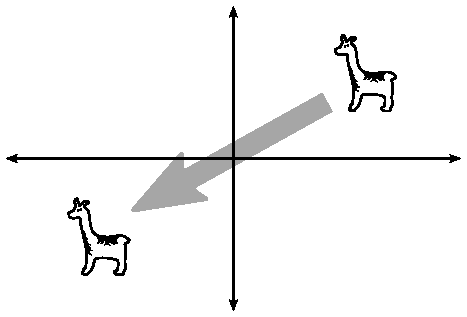
\includegraphics{../graphics/transIdeaEg.pdf}
\]

Pretty simple eh? We can give a more ``mathematical'' definition of a
translation involving our newly-found knowledge of matrices! Check it:

\begin{dfn}\index{translation}
A \textbf{translation}, denoted by $\mat{T}_{(u,v)}$, is a function
that moves every point a given distance $u$ in the $x$-direction and a
given distance $v$ in the $y$-direction. We will use the following
matrix to represent translations:
\[
\mat{T}_{(u,v)} = 
\begin{bmatrix}
1 & 0 & u \\ 
0 & 1 & v \\
0 & 0 & 1
\end{bmatrix}
\]
\end{dfn}


\begin{eg} 
Consider the point $\vec{p} = (-3,2)$. Use a matrix to translate
$\vec{p}$ $5$ units right and $4$ units down.
\[
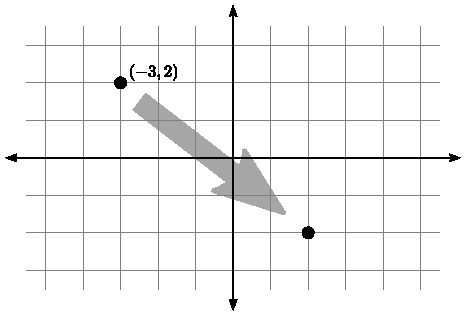
\includegraphics{../graphics/transEg1.pdf}
\]
Here is how you do it:
\begin{align*}
\mat{T}_{(5,-4)} \vec{p} &= 
\begin{bmatrix}
1 & 0 & 5 \\ 
0 & 1 & -4 \\
0 & 0 & 1
\end{bmatrix}
\begin{bmatrix}
-3 \\
2 \\
1
\end{bmatrix}\\
&=
\begin{bmatrix}
-3 + 0 + 5\\
0 + 2 - 4 \\
0 + 0 + 1
\end{bmatrix}\\
&=
\begin{bmatrix}
2\\
-2 \\
1
\end{bmatrix}
\end{align*}
Hence, we end up with the point $(2,-2)$. But you knew that already,
didn't you?
\end{eg}

\begin{ques} 
Can you demonstrate with algebra why translations are isometries?
\end{ques}
\QM


\begin{ques} 
We know how to translate individual points. How do we move entire
figures and other funky shapes?
\end{ques}
\QM


\subsection{Reflections}


The act of reflection has fascinated humanity for millennia.  It has a
strong effect on our perception of beauty and has a defined place in
art---not to mention how useful it is for the application
of make-up. Here is our definition of a reflection:

\begin{dfn}\index{reflection}
The \textbf{reflection} across a line $\l$, denoted by $\mat{F}_\l$, is the
function that maps a point $\vec{p}$ to a point $\mat{F}_\l
\vec{p}$ such that:
\begin{enumerate}
\item If $\vec{p}$ is on $\l$, then $\mat{F}_\l \vec{p} = \vec{p}$.
\item If $\vec{p}$ is not on $\l$, then $\l$ is the perpendicular
  bisector of the segment connecting $\vec{p}$ and $\mat{F}_\l \vec{p}$. 
\end{enumerate}
\end{dfn}

You might be saying, ``Huh?''  It's not as hard as it looks.  Check
out this picture of the situation; again Louie Llama\index{Louie Llama} 
will help us out:
\[
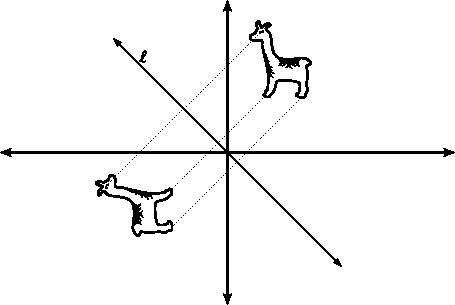
\includegraphics{../graphics/refIdeaEg.pdf}
\]

\subsubsection{A Collection of Reflections}

We are going to begin with a trio of reflections. We'll start with a
\textbf{horizontal reflection}\index{horizontal reflection}\index{reflection!horizontal} across the $y$-axis.  Using
our matrix notation, we write:
\[
\mat{F}_{x=0} =
\begin{bmatrix}
-1 & 0 & 0\\
 0 & 1 & 0\\
 0 & 0 & 1
\end{bmatrix}
\]

The next reflection in our collection is a \textbf{vertical
  reflection}\index{vertical reflection}\index{reflection!vertical}
across the $x$-axis.  Using our matrix notation, we write:
\[
\mat{F}_{y=0} =
\begin{bmatrix}
1 &  0 & 0\\
0 & -1 & 0\\
0 &  0 & 1
\end{bmatrix}
\]
The final reflection to add to our collection is a \textbf{diagonal
  reflection}\index{diagonal reflection}\index{reflection!diagonal}
across the line $y=x$.  Using our matrix notation, we write:
\[
\mat{F}_{y=x} =
\begin{bmatrix}
0 & 1 & 0\\
1 & 0 & 0\\
0 & 0 & 1
\end{bmatrix}
\]


\begin{eg}
Consider the point $\vec{p} =(3,-1)$.  Use a matrix to reflect
$\vec{p}$ across the line $y = x$.
\[
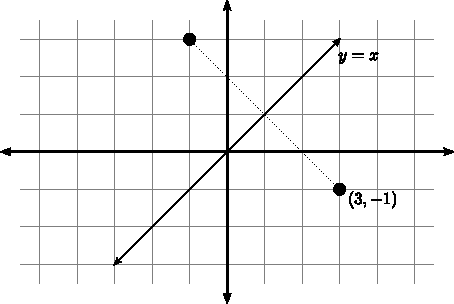
\includegraphics{../graphics/refEg1.pdf}
\]
Here is how you do it:
\begin{align*}
\mat{F}_{y = x} \vec{p} &= 
\begin{bmatrix}
0 & 1 & 0 \\ 
1 & 0 & 0 \\
0 & 0 & 1
\end{bmatrix}
\begin{bmatrix}
3 \\
-1 \\
1
\end{bmatrix}\\
&=
\begin{bmatrix}
0-1+0\\
3+0+0 \\
0+0+1
\end{bmatrix}\\
&=
\begin{bmatrix}
-1\\
3 \\
1
\end{bmatrix}
\end{align*}
Hence we end up with the point $(-1,3)$. 
\end{eg}

\begin{ques}
Let $\vec{p}$ be some point in Quadrant I of the $(x,y)$-plane. What
reflection will map this point to Quadrant II? What about Quadrant IV?
What about Quadrant III?
\end{ques}
\QM


\begin{ques} 
Can you demonstrate with algebra why each of our reflections above are
isometries?
\end{ques}
\QM




\subsection{Rotations}

Imagine that you are on a swing set, going higher and higher until you
are actually able to make a full circle\footnote{Face it, I think we
  all dreamed of doing that when we were little---or in my case, last
  week.}. At the point where you are directly above where you would be
if the swing were at rest, where is your head, comparatively?  Your
feet?  Your hands?


Rotations should bring circles to mind. This is not a
coincidence. Check out our definition of a \textit{rotation}:

\begin{dfn}\index{rotation}
A \textbf{rotation} of $\theta$ degrees about the origin, denoted by
$\mat{R}_\theta$, is a function that maps a point $\vec{p}$ to a point
$\mat{R}_\theta \vec{p}$ such that:
\begin{enumerate}
\item The points $\vec{p}$ and $\mat{R}_\theta \vec{p}$ are equidistant
  from the origin.
\item An angle of $\theta$ degrees is formed by $\vec{p}$, the origin, and
  $\mat{R}_\theta\vec{p}$.
\end{enumerate}
Louie Llama, can you do the honors?\index{Louie Llama}
\end{dfn}
\[
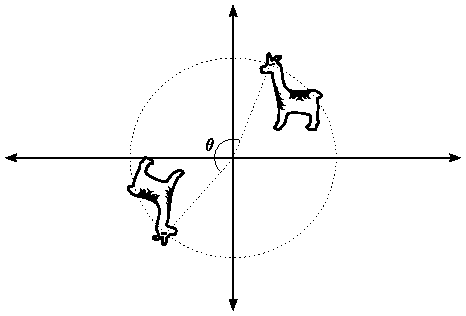
\includegraphics{../graphics/rotIdeaEg.pdf}
\]
\begin{war} 
Positive angles denote a counterclockwise rotation. Negative angles
denote a clockwise rotation.
\end{war}

Looking back on trigonometry, there were some angles that kept on
coming up. Some of these were $90^\circ$, $60^\circ$, and $45^\circ$.
We'll focus on these angles too.
\[
\mat{R}_{90} =
\begin{bmatrix}
0 & -1 & 0\\
1 & 0 & 0\\
0 & 0 & 1
\end{bmatrix}
\qquad 
\mat{R}_{60} =
\begin{bmatrix}
\frac{1}{2} & \frac{-\sqrt{3}}{2} & 0\\
\frac{\sqrt{3}}{2} & \frac{1}{2} & 0\\
0 & 0 & 1
\end{bmatrix}
\qquad
\mat{R}_{45} =
\begin{bmatrix}
\frac{1}{\sqrt{2}} & \frac{-1}{\sqrt{2}} & 0\\
\frac{1}{\sqrt{2}} & \frac{1}{\sqrt{2}} & 0\\
0 & 0 & 1
\end{bmatrix}
\]


\begin{eg} 
Consider the point $\vec{p} = (4,-2)$. Use a matrix to rotate
$\vec{p}$ $60^\circ$ about the origin.
\[
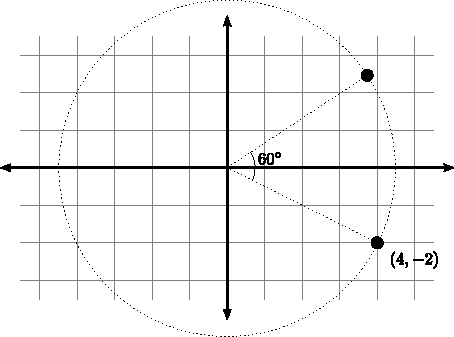
\includegraphics{../graphics/rotEg1.pdf}
\]
Here is how you do it:
\begin{align*}
\mat{R}_{60} \vec{p} &= 
\begin{bmatrix}
\frac{1}{2} & \frac{-\sqrt{3}}{2} & 0\\
\frac{\sqrt{3}}{2} & \frac{1}{2} & 0\\
0 & 0 & 1
\end{bmatrix}
\begin{bmatrix}
4 \\
-2 \\
1
\end{bmatrix}\\
&=
\begin{bmatrix}
2 +\sqrt{3} + 0\\
2\sqrt{3} -1 + 0 \\
0 + 0 + 1
\end{bmatrix}\\
&=
\begin{bmatrix}
2+\sqrt{3}\\
2\sqrt{3}-1 \\
1
\end{bmatrix}
\end{align*}
Hence, we end up with the point $(2+\sqrt{3},2\sqrt{3}-1)$.
\end{eg}


\begin{ques}
Do the numbers in the matrices above look familiar? If so, why?
\end{ques}
\QM

\begin{ques}
How do you rotate a point $180$ degrees?
\end{ques}
\QM


\begin{ques} 
Can you demonstrate with algebra why our rotations
above are isometries?
\end{ques}
\QM




\newpage


\problems
\begin{enumerate}
\item How do you compute the distance between two points $\vec{p}$ and
  $\vec{q}$ in the plane?
\item Use algebra to explain why: 
\[
d(\vec{p},\vec q) = d(\vec{p}-\vec q,\vec o) = d(\vec o,\vec{p}-\vec q)
\]
where $\vec o = (0,0)$.
\item What is an isometry?
\item What is a translation?
\item What is a rotation?
\item What is a reflection?
\item Reflecting back on this chapter, suppose I translate a point
  $\vec{p}$ to $\vec{p}'$. Does it make any difference if I move the
  point $\vec{p}$ along a wiggly path
\[
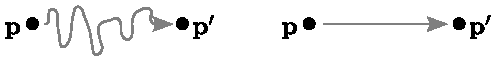
\includegraphics{../graphics/wiggle.pdf}
\]
or a straight path? Explain your reasoning.
\item Reflecting back on this chapter, is a rotation the continuous
  \textit{act} of \textit{moving} a point through an angle around some
  fixed point, or is it just a final picture compared to the initial
  one? Explain your reasoning.
\item In the vector illustrator \textit{Inkscape} there is an option
  to transform an image via a ``matrix.'' If you select this tool, you
  are presented with $6$ boxes to fill in with numbers:
\[
\begin{array}{|c|c|c|}
\hline
 & & \\
\hline
 & & \\
\hline
\end{array}
\]
Use what you've learned in this chapter to make a guess as to how this
tool works.
\item In what direction does a positive rotation occur?
\item Is a $270^\circ$ rotation the same as a $-90^\circ$ rotation?
  Explain your reasoning.
%\item Devise a way to explain translations using compass and
%  straightedge constructions.
%\item Devise a way to explain translations using origami
%  constructions.
%\item Devise a way to explain reflections using origami constructions.
%\item Devise a way to explain rotations using compass and straightedge
%  constructions.
\item Consider the following matrix:
\[
\mat{M} = 
\begin{bmatrix}
1 & 0 & 0\\
0 & 1 & 0\\
0 & 0 & 1
\end{bmatrix}
\]
Is $\mat{M}$ an isometry? Explain your reasoning.
\item Consider the following matrix:
\[
\mat{M} = 
\begin{bmatrix}
0 & 0 & 8\\
2 & 1 & 0\\
0 & 0 & 1
\end{bmatrix}
\]
Is $\mat{M}$ an isometry? Explain your reasoning.
\item Consider the following matrix:
\[
\mat{M} = 
\begin{bmatrix}
0  & -1  & 0\\
-1 & 0  & 0\\
0  & 0  & 1
\end{bmatrix}
\]
Is $\mat{M}$ an isometry? Explain your reasoning.
\item Consider the following matrix:
\[
\mat{M} = 
\begin{bmatrix}
0  & 2  & 0\\
-3 & 0  & 0\\
0  & 0  & 1
\end{bmatrix}
\]
\item Consider the following matrix:
\[
\mat{M} = 
\begin{bmatrix}
1  & 2  & 1\\
1 & 1  & 2\\
0  & 0  & 1
\end{bmatrix}
\]
Is $\mat{M}$ an isometry? Explain your reasoning.
\item Use a matrix to translate the point $(-1,6)$ three units right
  and two units up. Sketch this situation and explain your reasoning.
\item The matrix $\mat{T}_{(-2,6)}$ was used to translate the point
  $\vec{p}$ to $(-1,-3)$.  What is $\vec{p}$? Sketch this situation
  and explain your reasoning.
\item Use a matrix to reflect the point $(5,2)$ across the
  $x$-axis. Sketch this situation and explain your reasoning.
\item Use a matrix to reflect the point $(-3,4)$ across the
  $y$-axis. Sketch this situation and explain your reasoning.
\item Use a matrix to reflect the point $(-1,1)$ across the line
  $y=x$. Sketch this situation
  and explain your reasoning.
\item Use a matrix to reflect the point $(1,1)$ across the line
  $y=x$. Sketch this situation
  and explain your reasoning.
\item The matrix $\mat{F}_{y=0}$ was used to reflect the point $\vec{p}$
  to $(4,3)$.  What is $\vec{p}$? Explain your reasoning.
\item The matrix $\mat{F}_{y=0}$ was used to reflect the point $\vec{p}$
  to $(0,-8)$.  What is $\vec{p}$? Explain your reasoning.
\item The matrix $\mat{F}_{x=0}$ was used to reflect the point $\vec{p}$
  to $(-5,-1)$.  What is $\vec{p}$? Explain your reasoning.
\item The matrix $\mat{F}_{y=x}$ was used to reflect the point $\vec{p}$
  to $(9,-2)$.  What is $\vec{p}$? Explain your reasoning.
\item The matrix $\mat{F}_{y=x}$ was used to reflect the point $\vec{p}$
  to $(-3,-3)$.  What is $\vec{p}$? Explain your reasoning.
\item Considering the point $(3,2)$, use a matrix to rotate this point
  $60^\circ$ about the origin.  Sketch this situation and explain your
  reasoning.  
\item Considering the point $(\sqrt{2},-\sqrt{2})$, use a matrix to
  rotate this point $45^\circ$ about the origin.  Sketch this
  situation and explain your reasoning.
\item Considering the point $(-7,6)$, use a matrix to rotate this point
  $90^\circ$ about the origin.  Sketch this situation and explain your
  reasoning.  
\item Considering the point $(-1,3)$, use a matrix to rotate this point
  $0^\circ$ about the origin.  Sketch this situation and explain your
  reasoning.  
\item Considering the point $(0,0)$, use a matrix to rotate this point
  $120^\circ$ about the origin.  Sketch this situation and explain your
  reasoning.  
\item Considering the point $(1,1)$, use a matrix to rotate this point
  $-90^\circ$ about the origin.  Sketch this situation and explain your
  reasoning.  
\item The matrix $\mat{R}_{90}$ was used to rotate the point $\vec{p}$
  to $(2,-5)$.  What is $\vec{p}$? Explain your reasoning.
\item The matrix $\mat{R}_{60}$ was used to rotate the point $\vec{p}$
  to $(0,2)$.  What is $\vec{p}$? Explain your reasoning.
\item The matrix $\mat{R}_{45}$ was used to rotate the point $\vec{p}$
  to $(-\frac{1}{2}, \frac{5}{2})$.  What is $\vec{p}$? Explain your reasoning.
\item The matrix $\mat{R}_{-90}$ was used to rotate the point $\vec{p}$
  to $(4,3)$.  What is $\vec{p}$? Explain your reasoning.
\item If someone wanted to plot the graph of $y=x^2$, they might start
  by filling in the following table:
\[
\begin{array}{r | c}
 x & x^2 \\
\hline\hline
0  & \\\hline
1  & \\\hline
-1 & \\\hline
2  & \\\hline
-2 & \\\hline
3  & \\\hline
-3 & 
\end{array}
\]
Reflect each point you obtain from the table above about the line
$y=x$. Give a plot of this situation. What curve do you obtain? What
is this new curve's relationship to $y=x^2$? Explain your reasoning.
\item Some translation $\mat{T}$ was used to map point $\vec{p}$ to
  point $\vec{q}$.  Given $\vec{p}$ = $(1,2)$ and $\vec{q}$ = $(3,4)$,
  find $\mat{T}$ and explain your reasoning.
\item Some translation $\mat{T}$ was used to map point $\vec{p}$ to
  point $\vec{q}$.  Given $\vec{p}$ = $(-2,3)$ and $\vec{q}$ =
  $(2,3)$, find $\mat{T}$ and explain your reasoning.
\item Some reflection $\mat{F}$ was used to map point $\vec{p}$ to
  point $\vec{q}$.  Given $\vec{p}$ = $(1,4)$ and $\vec{q}$ =
  $(1,-4)$, find $\mat{F}$ and explain your reasoning.
\item Some reflection $\mat{F}$ was used to map point $\vec{p}$ to
  point $\vec{q}$.  Given $\vec{p}$ = $(5,0)$ and $\vec{q}$ = $(0,5)$,
  find $\mat{F}$ and explain your reasoning.
\item Some rotation $\mat{R}$ was used to map point $\vec{p}$ to point
  $\vec{q}$.  Given $\vec{p}$ = $(3,0)$ and $\vec{q}$ = $(0,3)$, find
  $\mat{R}$ and explain your reasoning.
\item Some rotation $\mat{R}$ was used to map point $\vec{p}$ to point
  $\vec{q}$.  Given $\vec{p}$ = $(\sqrt{2},\sqrt{2})$ and $\vec{q}$ =
  $(0,2)$, find $\mat{R}$ and explain your reasoning.
\item Some matrix $\mat{M}$ maps 
\begin{align*}
(0,0) &\mapsto (0,0), \\
(1,0) &\mapsto (3,0), \\
(0,1) &\mapsto (0,5).
\end{align*}
Find $\mat{M}$ and explain your reasoning.
\item Some matrix $\mat{M}$ maps 
\begin{align*}
(0,0) &\mapsto (-1,1), \\
(1,0) &\mapsto (3,0), \\
(0,1) &\mapsto (0,5).
\end{align*}
Find $\mat{M}$ and explain your reasoning.
\item Some matrix $\mat{M}$ maps 
\begin{align*}
(0,0) &\mapsto (1,1), \\
(1,0) &\mapsto (2,1), \\
(0,1) &\mapsto (1,2).
\end{align*}
Find $\mat{M}$ and explain your reasoning.
\item Some matrix $\mat{M}$ maps 
\begin{align*}
(0,0) &\mapsto (2,2), \\
(1,1) &\mapsto (3,3), \\
(-1,1) &\mapsto (1,3).
\end{align*}
Find $\mat{M}$ and explain your reasoning.
\item Some matrix $\mat{M}$ maps 
\begin{align*}
(0,0) &\mapsto (0,0), \\
(1,1) &\mapsto (0,3), \\
(-1,1) &\mapsto (5,0).
\end{align*}
Find $\mat{M}$ and explain your reasoning.
\item Some matrix $\mat{M}$ maps 
\begin{align*}
(0,0) &\mapsto (1,2), \\
(1,1) &\mapsto (-3,1), \\
(-1,1) &\mapsto (2,-3).
\end{align*}
Find $\mat{M}$ and explain your reasoning.

%\item\label{P:lineCoord}  Consider the line $3x+4y = 2$. 
%\begin{enumerate}
%\item If $\vec{p}$ is a point on the line, and the $x$-coordinate of
%  $\vec{p}$ is $6$, what is the $y$ coordinate?
%\item If $\vec{p}$ is a point on the line, and the $x$-coordinate of
%  $\vec{p}$ is $-3$, what is the $y$ coordinate?
%\item If $\vec{p}$ is a point on the line, what are the coordinates of
%  $\vec{p}$ purely in terms of $x$?
%\item Now consider the line $ax+by = c$. If $\vec{p}$ is a point on
%  the line, what are the coordinates of $\vec{p}$ in terms of $x$ and
%  $y$?
%\end{enumerate}
%\item Consider $\mat{T}_{(u,v)}$ and a line $\l: ax + by = c$. Use
%  algebra to explain why $\mat{T}_{(u,v)}\l$ is a new line and not
%  some other curve. Hint: See Problem~\ref{P:lineCoord}.
%\item Consider $\mat{T}_{(u,v)}$ and a line $\l: ax + by = c$. Use
%  algebra to explain why $\mat{T}_{(u,v)}\l$ is a new line that is
%  parallel to the original line. Hint: See Problem~\ref{P:lineCoord}.
\end{enumerate}

\newpage








\section{The Algebra of Matrices}


\subsection{Matrix Multiplication}

We know how to multiply a matrix and a point. Multiplying two
matrices is a similar procedure:
\[
\begin{bmatrix}
a & b & c \\ 
d & e & f \\
g & h & i
\end{bmatrix}
\begin{bmatrix}
j & k & l \\ 
m & n & o \\
p & q & r
\end{bmatrix}
= \begin{bmatrix}
aj + bm + cp & ak + bn + cq & al + bo + cr \\
dj + em + fp & dk + en + fq & dl + eo + fr \\
gj + hm + ip & gk + hn + iq & gl + ho + ir 
\end{bmatrix}
\]

Variables are all good and well, but let's do this with actual
numbers. Consider the following two matrices:
\[
\mat{M} =
\begin{bmatrix}
1 & 2 & 3\\
4 & 5 & 6\\
7 & 8 & 9
\end{bmatrix}
\qquad\text{and}\qquad
\mat{I} = 
\begin{bmatrix}
1 & 0 & 0\\
0 & 1 & 0\\
0 & 0 & 1
\end{bmatrix}
\]
Let's multiply them together and see what we get:
\begin{align*}
\mat{M}\mat{I} &= \begin{bmatrix}
1 & 2 & 3\\
4 & 5 & 6\\
7 & 8 & 9
\end{bmatrix}
\begin{bmatrix}
1 & 0 & 0\\
0 & 1 & 0\\
0 & 0 & 1
\end{bmatrix} \\
&=
\begin{bmatrix}
1\cdot 1 + 2\cdot 0 + 3\cdot 0 & 1\cdot 0 + 2\cdot 1 + 3\cdot 0 & 1\cdot 0 + 2\cdot 0 + 3\cdot 1\\
4\cdot 1 + 5\cdot 0 + 6\cdot 0 & 4\cdot 0 + 5\cdot 1 + 6\cdot 0 & 4\cdot 0 + 5\cdot 0 + 6\cdot 1\\
7\cdot 1 + 8\cdot 0 + 9\cdot 0 & 7\cdot 0 + 8\cdot 1 + 9\cdot 0 & 7\cdot 0 + 8\cdot 0 + 9\cdot 1 
\end{bmatrix} \\
&=
\begin{bmatrix}
1 & 2 & 3\\
4 & 5 & 6\\
7 & 8 & 9
\end{bmatrix} \\
&= \mat{M}
\end{align*}

\begin{ques}
What is $\mat{I}\mat{M}$ equal to?
\end{ques}
\QM 

It turns out that we have a special name for $\mat{I}$.  We call it the \textbf{identity matrix}.\index{identity matrix}

\begin{war}
Matrix multiplication is \textbf{not} generally commutative. Check it out:
\[
\mat{F} =
\begin{bmatrix}
1 & 0 & 0\\
0 & -1 & 0\\
0 & 0 & 1
\end{bmatrix}
\qquad\text{and}\qquad
\mat{R} = 
\begin{bmatrix}
0 & -1 & 0\\
1 & 0 & 0\\
0 & 0 & 1
\end{bmatrix}
\]
When we multiply these matrices, we get:
\begin{align*}
\mat{F}\mat{R} &= \begin{bmatrix}
1 & 0 & 0\\
0 & -1 & 0\\
0 & 0 & 1\\
\end{bmatrix}
\begin{bmatrix}
0 & -1 & 0\\
1 & 0 & 0\\
0 & 0 & 1\\
\end{bmatrix} \\
&=
\begin{bmatrix}
1\cdot 0 +  0\cdot 1 + 0\cdot 0 & 1\cdot (-1) +  0\cdot 0 + 0\cdot 0 & 1\cdot 0 +  0\cdot 0 + 0\cdot 1\\
0\cdot 0 + (-1)\cdot 1 + 0\cdot 0 & 0\cdot (-1) + (-1)\cdot 0 + 0\cdot 0 & 0\cdot 0 + (-1)\cdot 0 + 0\cdot 1\\
0\cdot 0 +  0\cdot 1 + 1\cdot 0 & 0\cdot (-1) +  0\cdot 0 + 1\cdot 0 & 0\cdot 0 +  0\cdot 0 + 1\cdot 1\\
\end{bmatrix} \\
&=
\begin{bmatrix}
0 & -1 & 0\\
-1 & 0 & 0\\
0 & 0 & 1\\
\end{bmatrix}
\end{align*}
On the other hand, we get:
\[
\mat{R}\mat{F} = \begin{bmatrix}
0 & 1 & 0\\
1 & 0 & 0\\
0 & 0 & 1
\end{bmatrix}
\]
\end{war}

\begin{ques}
Can you draw some nice pictures showing geometrically that matrix
multiplication is not commutative?
\end{ques}
\QM

\begin{ques}
Is it always the case that $(\mat{L}\mat{M})\mat{N} = \mat{L}(\mat{M}\mat{N})$?
\end{ques}
\QM




\subsection{Compositions of Matrices}

It is often the case that we wish to apply several isometries
successively to a point. Consider the following:
\[
\mat{M} =
\begin{bmatrix}
a & b & c\\
d & e & f \\
0 & 0 & 1
\end{bmatrix}
\qquad
\mat{N} =
\begin{bmatrix}
g & h & i\\
j & k & l\\
0 & 0 & 1
\end{bmatrix}
\qquad\text{and}\qquad \vec{p} =
\begin{bmatrix}
x \\
y \\
1
\end{bmatrix}
\]
Now let's compute 
\begin{align*}
\mat{M}(\mat{N}\vec{p}) &= \begin{bmatrix}
a & b & c\\
d & e & f \\
0 & 0 & 1
\end{bmatrix} 
\left(
\begin{bmatrix}
g & h & i\\
j & k & l\\
0 & 0 & 1
\end{bmatrix}
\begin{bmatrix}
x \\
y \\
1
\end{bmatrix}
\right)\\
&= 
\begin{bmatrix}
a & b & c\\
d & e & f \\
0 & 0 & 1
\end{bmatrix} 
\begin{bmatrix}
gx+hy + i\\
jx+ky +l\\
1
\end{bmatrix} \\
&=
\begin{bmatrix}
agx+ahy +ai + bjx+bky+bl+c\\
dgx+dhy+ di + ejx+eky+el+f\\
1
\end{bmatrix}
\end{align*}
Now \textit{you} compute $(\mat{M}\mat{N})\vec{p}$ and compare what
\textit{you} get to what we got above.



\subsubsection{Compositions of Translations}

A composition of translations occurs when two or more successive
translations are applied to the same point. Check it out:
\begin{align*}
\mat{T}_{(5,-4)}\mat{T}_{(-3,2)} &= \begin{bmatrix}
1 & 0 &  5\\
0 & 1 & -4\\
0 & 0 &  1
\end{bmatrix}
\begin{bmatrix}
1 & 0 & -3\\
0 & 1 &  2\\
0 & 0 &  1
\end{bmatrix}\\
&=\begin{bmatrix}
1 & 0 &  2\\
0 & 1 & -2\\
0 & 0 &  1
\end{bmatrix}\\
&=\mat{T}_{(5+(-3),(-4)+2)}\\
&=\mat{T}_{(2,-2)}
\end{align*}

\begin{thm}
The composition of two translations $\mat{T}_{(u,v)}$ and
$\mat{T}_{(s,t)}$ is equal to the translation $\mat{T}_{(u+s,v+t)}$.
\end{thm}

\begin{ques} How do you prove the theorem above?
\end{ques}
\QM

\begin{ques}
Can you give a single translation that is equal to the following composition?
\[
\mat{T}_{(-7,5)}\mat{T}_{(0,-6)}\mat{T}_{(2,8)}\mat{T}_{(5,-4)}
\]
\end{ques}
\QM

\begin{ques}
Are compositions of translations commutative?  Are they
associative?
\end{ques}
\QM


\subsubsection{Compositions of Reflections}

A composition of reflections occurs when two or more successive
reflections are applied to the same point. Check it out:

\begin{align*}
\mat{F}_{y=0}\mat{F}_{y=x} &= \begin{bmatrix}
1 &  0 & 0\\
0 & -1 & 0\\
0 &  0 & 1
\end{bmatrix}
\begin{bmatrix}
0 & 1 & 0\\
1 & 0 & 0\\
0 & 0 & 1
\end{bmatrix}\\
&= \begin{bmatrix}
 0 & 1 & 0\\
-1 & 0 & 0\\
 0 & 0 & 1
\end{bmatrix}
\end{align*}


\begin{ques}
Is the composition $\mat{F}_{y=0}\mat{F}_{y=x}$ still a reflection?
\end{ques}
\QM

\begin{ques}
Are compositions of reflections commutative?  Are they
associative?
\end{ques}
\QM



\subsubsection{Compositions of Rotations}


A composition of rotations occurs when two or more successive
rotations are applied to the same point. Check it out: 
\begin{align*}
\mat{R}_{60}\mat{R}_{60} &= \begin{bmatrix}
\frac{1}{2} & \frac{-\sqrt{3}}{2} & 0\\
\frac{\sqrt{3}}{2} & \frac{1}{2} & 0\\
0 & 0 & 1
\end{bmatrix}
\begin{bmatrix}
\frac{1}{2} & \frac{-\sqrt{3}}{2} & 0\\
\frac{\sqrt{3}}{2} & \frac{1}{2} & 0\\
0 & 0 & 1
\end{bmatrix}\\
&= \begin{bmatrix}
\frac{-1}{2} & \frac{-\sqrt{3}}{2} & 0\\
\frac{\sqrt{3}}{2} & \frac{-1}{2} & 0\\
0 & 0 & 1
\end{bmatrix}
\end{align*}

\begin{thm}
The product of two rotations $\mat{R}_\theta$ and $\mat{R}_\ph$ is
equal to the rotation $\mat{R}_{\theta+\ph}$.
\end{thm}

From this we see that:
\[
\mat{R}_{120} =
\begin{bmatrix}
\frac{-1}{2} & \frac{-\sqrt{3}}{2} & 0\\
\frac{\sqrt{3}}{2} & \frac{-1}{2} & 0\\
0 & 0 & 1
\end{bmatrix}
\]

\begin{ques} What is the rotation matrix for a $360^\circ$ rotation? What about a $405^\circ$ rotation?
\end{ques}
\QM

\begin{ques}
Are compositions of rotations commutative?  Are they
associative?
\end{ques}
\QM



\subsection{Mixing and Matching}

Life gets interesting when we start composing translations,
reflections, and rotations together.  First we'll compose a reflection
with a rotation:

\begin{align*}
\mat{F}_{y=0}\mat{R}_{60} &= \begin{bmatrix}
1 &  0 & 0\\
0 & -1 & 0\\
0 &  0 & 1
\end{bmatrix}
\begin{bmatrix}
\frac{1}{2} & \frac{-\sqrt{3}}{2} & 0\\ \frac{\sqrt{3}}{2} &
\frac{1}{2} & 0\\ 0 & 0 & 1
\end{bmatrix}\\
&= \begin{bmatrix}
\frac{1}{2} & \frac{-\sqrt{3}}{2} & 0\\
-\frac{\sqrt{3}}{2} & -\frac{1}{2} & 0\\
0 & 0 & 1
\end{bmatrix}
\end{align*}

\begin{ques}
Does this result look familiar?
\end{ques}
\QM

Now how about a rotation composed with a translation:

\begin{align*}
\mat{R}_{90}\mat{T}_{(3,-4)} &= \begin{bmatrix}
0 & -1 & 0\\
1 & 0 & 0\\
0 & 0 & 1
\end{bmatrix}
\begin{bmatrix}
1 & 0 & 3\\
0 & 1 & -4\\
0 & 0 & 1
\end{bmatrix}\\
&=
\begin{bmatrix}
0 & -1 & 4\\
1 & 0 & 3\\
0 & 0 & 1
\end{bmatrix}
\end{align*}

\begin{ques}
Does $\mat{R}_{90}\mat{T}_{(3,-4)}= \mat{T}_{(3,-4)}\mat{R}_{90}$?
\end{ques}
\QM

\begin{ques} Find a matrix that represents the reflection $\mat{F}_{y=-x}$.
\end{ques}

I'll take this one. Note that 
\begin{align*}
\mat{F}_{y=-x} &= \mat{R}_{180} \mat{F}_{y=x} \\
&= \mat{R}_{90}\mat{R}_{90} \mat{F}_{y=x}\\
&= \begin{bmatrix}
0 & -1 & 0\\
1 & 0 & 0\\
0 & 0 & 1
\end{bmatrix}
\begin{bmatrix}
0 & -1 & 0\\
1 & 0 & 0\\
0 & 0 & 1
\end{bmatrix}
\begin{bmatrix}
0&  1 & 0\\
1 & 0 & 0\\
0 &  0 & 1
\end{bmatrix} \\
&=\begin{bmatrix}
0 &  -1 & 0\\
-1 & 0 & 0\\
0 &  0 & 1
\end{bmatrix} 
\end{align*}
OK, looks good.  But you, the reader, are going to have to check the
above computation yourself.



\begin{ques} 
How do we deal with reflections that are not across the lines $y=0$,
$x=0$, or $y=x$? How would you reflect points across the line $y = 1$?
\end{ques}
\QM





\newpage

\problems

\begin{enumerate}
\item Give a single translation that is equal to
  $\mat{T}_{(-3,2)}\mat{T}_{(5,-1)}$. Explain your reasoning.
\item Consider the two translations $\mat{T}_{(-4,8)}$ and
  $\mat{T}_{(4,-8)}$.  Do these commute?  Explain your reasoning.
\item Give a single reflection that is equal to
  $\mat{F}_{x=0}\mat{F}_{y=0}$. Sketch this situation and
  explain your reasoning.
\item Given any point $\vec{p} = (x,y)$, express
  $\mat{T}_{(4,2)}\mat{T}_{(6,-5)}\vec{p}$ as $\mat{T}_{(u,v)}\vec{p}$
  for some values of $u$ and $v$. Sketch this situation and explain
  your reasoning.
\item Give a matrix for $\mat{R}_{-45}$. Explain your reasoning.
\item Give a matrix for $\mat{R}_{-60}$. Explain your reasoning.
\item Sam suggests that:
\[
\mat{R}_{-90} = 
\begin{bmatrix}
0 & 1 & 0 \\
-1 & 0 & 0 \\ 
0 & 0 & 1
\end{bmatrix}
\]
Why does he suggest this? Is it even true? Explain your reasoning.
\item Give a matrix for $\mat{F}_{y=-x}$. Explain your reasoning.
\item Given the point $\vec{p}=(-4,2)$, use matrices to compute
  $\mat{F}_{y=0}\mat{F}_{y=x}\vec{p}$. Sketch this situation and
  explain your reasoning.
\item Given the point $\vec{p}=(5,0)$, use matrices to compute
  $\mat{F}_{y=x}\mat{F}_{y=-x}\vec{p}$. Sketch this situation and
  explain your reasoning.
\item Give a single rotation that is equal to
  $\mat{R}_{45}\mat{R}_{60}$. Explain your reasoning.
\item Given the point $\vec{p}=(1,3)$, use matrices to compute
  $\mat{R}_{45}\mat{R}_{90}\vec{p}$.  Sketch this situation and
  explain your reasoning.
\item Given the point $\vec{p}=(-7,2)$, use matrices to compute
  $\mat{R}_{45}\mat{R}_{-45}\vec{p}$.  Sketch this situation and
  explain your reasoning.
\item Given the point $\vec{p}=(-2,5)$, use matrices to compute
  $\mat{R}_{90}\mat{R}_{-90}\mat{R}_{360}\vec{p}$.  Sketch this
  situation and explain your reasoning.
\item Given the point $\vec{p}=(5,4)$, use matrices to compute
  $\mat{F}_{y=0}\mat{T}_{(2,-4)}\vec{p}$.  Sketch this
  situation and explain your reasoning.
\item Given the point $\vec{p}=(-1,6)$, use matrices to compute
  $\mat{R}_{45}\mat{T}_{(0,0)}\vec{p}$.  Sketch this situation and
  explain your reasoning.
\item Given the point $\vec{p}=(11,13)$, use matrices to  compute
  $\mat{T}_{(-6,-3)}\mat{R}_{135}\vec{p}$.  Sketch this situation and
  explain your reasoning.
\item Given the point $\vec{p}=(-7,-5)$, use matrices to compute
  $\mat{R}_{540}\mat{F}_{x=0}\vec{p}$.  Sketch this situation and
  explain your reasoning.



\item Give a composition of matrices that will take a
  point and reflect it across the $x$-axis and then rotate the result
  $90^\circ$ around the origin. Sketch this situation and
  explain your reasoning.

\item Give a composition of matrices that will take a
  point and translate it three units up and 2 units left and then
  rotate it $90^\circ$ clockwise around the origin. Sketch this situation and
  explain your reasoning.

\item Give a composition of matrices that will take a
  point and rotate it $270^\circ$ around the origin, reflect it across
  the line $y=x$, and then translate the result down 5 units and 3
  units to the right. Sketch this situation and
  explain your reasoning.

\item Give a composition of translations and any of the following matrices
\[
\{\mat{F}_{x=0},\mat{F}_{y=0}, \mat{F}_{y=x}, \mat{R}_{90},\mat{R}_{60},\mat{R}_{45}\}
\]
that will take a point and reflect it across the line $x=1$. Sketch
this situation and explain your reasoning.

\item Give a composition of translations and any of the following
  matrices
\[
\{\mat{F}_{x=0},\mat{F}_{y=0}, \mat{F}_{y=x}, \mat{R}_{90},\mat{R}_{60},\mat{R}_{45}\}
\]
that will take a point and reflect it across the line $y=-4$. Sketch
this situation and explain your reasoning.

\item Give a composition of translations and any of the following matrices
\[
\{\mat{F}_{x=0},\mat{F}_{y=0}, \mat{F}_{y=x}, \mat{R}_{90},\mat{R}_{60},\mat{R}_{45}\}
\]
that will take a
  point and reflect it across the line $y=x+5$. Sketch this situation
  and explain your reasoning.

\item Give a composition of translations and any of the following matrices
\[
\{
\mat{F}_{x=0},\mat{F}_{y=0}, \mat{F}_{y=x}, \mat{R}_{90},\mat{R}_{60},\mat{R}_{45}\}
\]
that will take a point and rotate it $45^\circ$ around the point
$(2,3)$. Sketch this situation and explain your reasoning.

\item Give a composition of translations and any of the following matrices
\[
\{\mat{F}_{x=0},\mat{F}_{y=0}, \mat{F}_{y=x}, \mat{R}_{90},\mat{R}_{60},\mat{R}_{45}\}
\]
that will take a point and rotate it $90^\circ$ clockwise around the
point $(-3,4)$ Sketch this situation and explain your reasoning.

\end{enumerate}



\newpage





\section{Symmetry}\index{symmetry}


\begin{ques}
What is \textit{symmetry}?
\end{ques}

You should think about the question above \textbf{before} reading
on---though, uncharistically, we will give an answer eventually.
Let's start by giving some examples of symmetry. An object can have
symmetry \textit{through reflections}:
\[
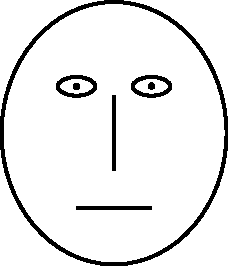
\includegraphics{../graphics/creepFace.pdf}
\]
Check it out---if the nose is along line line $x=0$, then the
reflection $\mat{F}_{x=0}$ does not change the picture.

An object can have symmetry \textit{through rotations}:
\[
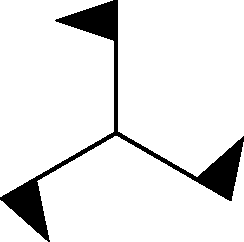
\includegraphics{../graphics/rotFlags.pdf}
\]
Check it out---if this object is centered at the origin, then the
rotation $\mat{R}_{120}$ does not change the picture.


An object can have symmetry \textit{through translations} if it
extends infinitely in some direction.  Imagine the pattern
below extending infinitely both to the left and the right:
\[
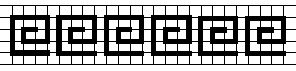
\includegraphics{../graphics/fpGraphEx1.pdf}
\]
Now the translation $\mat{T}_{(4,0)}$ does not change the
picture---note, we assumed that each square above is 1 unit.

\begin{ques}
What other translations don't change the picture?
\end{ques}
\QM


An object can have symmetry \textit{through dilations}.  Here we need
to imagine the entire plane filled with tiles as below:
\[
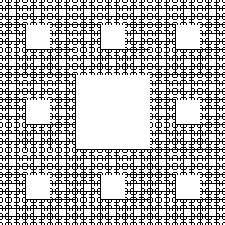
\includegraphics{../graphics/sierpinskiCarpet.pdf}
\]
This picture (assuming it extended infinitely) would have symmetry
through $\mat{D}_s$ for some scale factor $s$, see Activity~\ref{A:dilation}.


Trying to combine all these different ideas of symmetry is not easy.
In \cite{rosen}, it is said
\begin{center}\index{symmetry}
\textbf{Symmetry is immunity to a possible change.}
\end{center}

\begin{ques}
Can you explain what the definition of symmetry above is saying?
\end{ques}
\QM

\subsection{Symmetry Groups}

One of the most fundamental notions in all of modern mathematics is
that of a \textit{group}. Sadly, many students never see a group in their
education.

\begin{dfn}\index{group}
A \textbf{group} is a set of elements (in our case matrices) which we
will call $\mathcal{G}$ such that: 
\begin{enumerate}
\item There is an associative operation (in our case matrix multiplication).
\item The set is closed under this operation (the product of any two
  matrices in the set is also in the set).
\item There exists an identity $\mat{I}$ in $\mathcal{G}$ such that for all $\mat{M}$ in $\mathcal{G}$, 
\[
\mat{I}\mat{M}=\mat{M}\mat{I} = \mat{M}.
\]
\item For all $M$ in $\mathcal{G}$ there is an inverse $\mat{M}^{-1}$ in $\mathcal{G}$ such that 
\[
\mat{M} \mat{M}^{-1}= \mat{M}^{-1}\mat{M}= \mat{I}.
\]
\end{enumerate}
\end{dfn}


\subsection{Groups of Rotations}


Let's see an example of a group. Here we have an equilateral triangle centered at
the origin of the $(x,y)$-plane:
\[
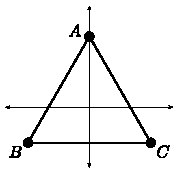
\includegraphics{../graphics/symTri.pdf}
\]
\begin{ques}
The matrix $\mat{R}_{360}$ will rotate this triangle completely
around the origin. What matrix will rotate this triangle one-third of
a complete rotation?
\end{ques}

As a gesture of friendship, I'll take this one. One-third of $360$ is
$120$. So we see that $\mat{R}_{120}$ will rotate the triangle one-third
of a full rotation. Do you remember this matrix? Here it is:
\[
\mat{R}_{120} =
\begin{bmatrix}
\frac{-1}{2} & \frac{-\sqrt{3}}{2} & 0\\
\frac{\sqrt{3}}{2} & \frac{-1}{2} & 0\\
0 & 0 & 1
\end{bmatrix}
\]
In spite of the fact that this matrix is messy and that matrix
multiplication is somewhat tedious, you should realize that
\[
\mat{R}_{120}^2 = \mat{R}_{240}\qquad\text{and}\qquad\mat{R}_{120}^3 = \mat{R}_{360}.
\]
Let's put these facts (and a few more) together in what is called a
\textit{group table}\index{group table}. Remember multiplication
tables from elementary school? Well, we're going to make something
like a ``multiplication table'' of rotations. We'll start by listing
the identity and powers of a one-third rotation along the top and
left-hand sides. Setting $\mat{R} = \mat{R}_{120}$ we have:
\[
{
\renewcommand{\arraystretch}{1.2}
\begin{array}{|c||c|c|c|c|c}
\hline 
\circ & \mat{I} & \mat{R} & \mat{R}^2 & \mat{R}^3 & \cdots \\ \hline\hline 
\mat{I} & & & & &  \\ \hline 
\mat{R} & & & & &  \\ \hline 
\mat{R}^2 &  & & & & \\ \hline
\mat{R}^3 &  & & & & \\ \hline
\vdots &  & & & & \\ 
\end{array}}
\]
Since $\mat{R}^3 = \mat{I}$, we need only take our table to
$\mat{R}^2$. In each entry of the table, we write the element we get by multiplying the row heading by the column heading.  (Since matrix multiplication isn't commutative, this is important!)  Now we can write out the complete table:
\[
{
\renewcommand{\arraystretch}{1.2}
\begin{array}{| c || c | c | c |}
\hline 
\circ & \mat{I} & \mat{R} & \mat{R}^2 \\ \hline\hline 
\mat{I} & \mat{I} & \mat{R} & \mat{R}^2 \\ \hline 
\mat{R} & \mat{R} & \mat{R}^2 & \mat{I} \\ \hline 
\mat{R}^2 & \mat{R}^2 & \mat{I} & \mat{R} \\ \hline
\end{array}}
\]
Since matrix multiplication is associative, and we see from the table
that every element has an inverse, we see that 
\[
\{\mat{I}, \mat{R}, \mat{R}^2\}
\]
is a group.

\begin{ques} 
What rotation matrices would we use when working with a square?  A
pentagon?  A hexagon?
\end{ques}
\QM


\subsection{Groups of Reflections}

Let's see another group. Again consider an equilateral triangle.  This
time we are interested in the three lines of reflection that preserve
this triangle:
\[
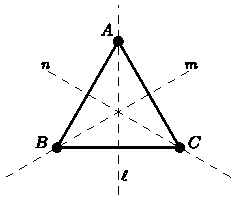
\includegraphics{../graphics/symTriRef.pdf}
\]

\begin{ques}
Suppose that the triangle above is centered at the origin of the
$(x,y)$-plane. What are equations for $\l$, $m$,
and $n$?
\end{ques}
\QM

The easiest of the reflections above is the reflection over
$\mat{F}_{\l}$.
\[
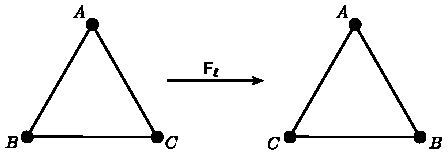
\includegraphics{../graphics/symTriRef1.pdf}
\]
We'll start our group table off with just two elements: $\mat{I}$ and
$\mat{F}=\mat{F}_{\l}$.

\[
\begin{array}{| c || c | c |}\hline
\circ & \mat{I} & \mat{F} \\ \hline\hline
\mat{I} & \mat{I} & \mat{F} \\\hline
\mat{F} & \mat{F} & \mat{I} \\ \hline
\end{array}
\]

Notice that when we apply $\mat{F}$ twice we're right back where we
started. Hence, $\mat{F} \mat{F} = \mat{I}$. Since matrix
multiplication is associative, we see that
\[
\{ \mat{I}, \mat{F} \}
\]
forms a group. Specifically this is a group of reflections of the
triangle.

\begin{ques} 
Above we used $\mat{F}_\l$. What would happen if we used $\mat{F}_m$
or $\mat{F}_n$? Also, what are the equations for the lines of symmetry
of the square centered at the origin?
\end{ques}
\QM







\subsection{Symmetry Groups}

Now let's mix our rotations and reflections.  Consider our original
triangle and apply $\mat{F}_\ell \mat{R}_{120}$:
\[
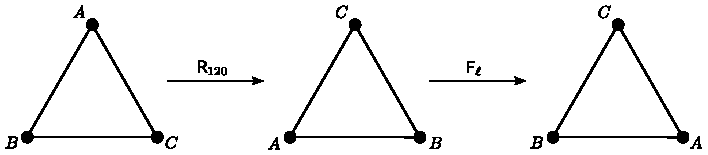
\includegraphics{../graphics/symTriComp1.pdf}
\]
What you may not immediately notice is that we obtain the same
transformation by taking the original triangle and applying
$\mat{F}_m$.
%\[
%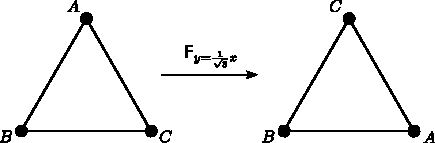
\includegraphics{../graphics/symTriComp2.pdf}
%\]



As it turns out, every possible symmetry of the equilateral triangle
can be represented using reflections and rotations.  Each of these
reflections and rotations can be expressed as a composition of a
single reflection and a single rotation.  The collection of all
symmetries forms a group called the \index{symmetry
  group}\textit{symmetry group} of the equilateral triangle. 
\[
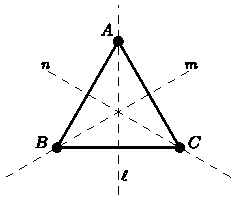
\includegraphics{../graphics/symTriRef.pdf}
\]
Let's see the group table.  Remember that we let $\mat{R} = \mat{R}_{120}$
and $\mat{F} = \mat{F}_{\l}$:

\[
{
\renewcommand{\arraystretch}{1.2}
\begin{array}{| c || c | c | c |c | c | c |}
\hline
\circ & \mat{I} & \mat{R} & \mat{R}^2  & \mat{F} & \mat{F} \mat{R} &  \mat{F} \mat{R}^2  \\ \hline \hline
\mat{I} & \mat{I} & \mat{R} & \mat{R}^2 & \mat{F} & \mat{F} \mat{R} & \mat{F} \mat{R}^2 \\ \hline
\mat{R} & \mat{R} & \mat{R}^2 & \mat{I} & \mat{F} \mat{R}^2 & \mat{F} & \mat{F} \mat{R} \\ \hline
\mat{R}^2 & \mat{R}^2 & \mat{I} & \mat{R} & \mat{F} \mat{R} & \mat{F} \mat{R}^2 & \mat{F}  \\ \hline
\mat{F} & \mat{F} & \mat{F} \mat{R} & \mat{F} \mat{R}^2 & \mat{I} & \mat{R} & \mat{R}^2 \\ \hline
\mat{F} \mat{R} & \mat{F} \mat{R} & \mat{F} \mat{R}^2 & \mat{F} & \mat{R}^2 & \mat{I} & \mat{R}  \\ \hline
\mat{F} \mat{R}^2 & \mat{F} \mat{R}^2 & \mat{F} & \mat{F} \mat{R} & \mat{R} & \mat{R}^2 & \mat{I}\\ \hline
\end{array}}
\]

This table shows every symmetry of the triangle, including the
identity $\mat{I}$. By comparing the rows and columns of the group
table, you can see that every element has an inverse. Combined
with the fact that the matrix multiplication is associative, this shows that
the symmetries of the triangle,
\[
\{ \mat{I},\mat{R},\mat{R}^2,\mat{F},\mat{F} \mat{R},  \mat{F} \mat{R}^2\}
\]
form a group.

\begin{ques} 
Can you express the symmetries of the square in terms of reflections
and rotations? What does the group table look like for the symmetry
group of the square?
\end{ques}
\QM



\newpage

\problems
\begin{enumerate}
\item Explain what \textit{symmetry} is.
\item State the definition of a group of matrices.
\item How many lines of reflectional symmetry exist for a square?
  Provide a drawing to justify your answer.
\item What are the equations for the lines of reflectional symmetry that exist for
  the square? Explain your answers.
\item How many lines of reflectional symmetry exist for a regular hexagon?  Provide a
  drawing to justify your answer.
\item What are the equations for the lines of reflectional symmetry
  for a regular hexagon?  Explain your answers.
%\item Give the group table for the rotations of a square.
%\item Give the group table for the rotations of a regular hexagon.
%\item Give the group table for the reflections of a square.
%\item Give the group table for the reflections of a regular hexagon.
%\item Give the group table for the symmetries of a square.
%\item Give the group table for the symmetries of a regular hexagon.
\item How many consecutive rotations are needed to return the vertices
  of a square to their original position? Provide a drawing to justify
  your answer, labeling the vertices.
\item How many degrees are in one-fourth of a complete rotation of the
  square?  Explain your answer.
\item How many degrees are in one-sixth of a complete rotation of the
  regular hexagon?  Explain your answer.
\item In this section, we've focused on a 3-sided figure, a 4-sided
  figure, and a 6-sided figure.  Why do we not include the rotation
  group for the pentagon in this section?  If we did, how many degrees
  would be in one-fifth of a complete rotation?
\item With the notation used in this section, draw pictures representing
  the action of each of $\mat{F}_\l$, $\mat{R}$,
  $\mat{R}\mat{F}_\l$ and $\mat{F}_\l\mat{R}$ on the equilateral
  triangle.
\item Consider a square centered at the origin. Draw pictures
  representing the action of $\mat{F}_{y=0}$, $\mat{R}_{90}$,
  $\mat{R}_{90}\mat{F}_{y=0}$, and $\mat{F}_{y=0} \mat{R}_{90}$ on
  this square.
\item Consider a regular hexagon centered at the origin. Draw pictures
  representing the action of $\mat{F}_{x=0}$, $\mat{R}_{60}$,
  $\mat{R}_{60}\mat{F}_{x=0}$, and $\mat{F}_{x=0} \mat{R}_{60}$ on
  this hexagon.
\item Find two symmetries of the equilateral triangle, neither of
  which is the identity, such that their composition is
  $\mat{R}_{120}$. Explain and illustrate your answer.
\item Find two symmetries of the equilateral triangle, neither of
  which is the identity, such that their composition is
  $\mat{F}_{x=0}$. Explain and illustrate your answer.
\item Find two symmetries of the equilateral triangle, neither of
  which is the identity, such that their composition is
  $\mat{R}_{120}^2$. Explain and illustrate your answer.
\item Find two symmetries of the square, neither of which is the
  identity, such that their composition is $\mat{R}_{180}$. Explain
  and illustrate your answer.
\item Find two symmetries of the square, neither of which is the
  identity, such that their composition is $\mat{F}_{\l}$.  The line $\l$ is a vertical line through the center of the square. Explain
  and illustrate your answer.
\item Find two symmetries of the square, neither of which is the
  identity, such that their composition is $\mat{R}_{270}$. Explain
  and illustrate your answer.
\item Use a group table to help you write out the symmetries of the
  equilateral triangle. List all elements that commute with every
  other element in the table. Explain your reasoning.
\item Use a group table to help you write out the symmetries of the
  square. List all elements that commute with every other element in
  the table. Explain your reasoning.
\item Use a group table to help you write out the symmetries of the
  regular hexagon. List all elements that commute with every other
  element in the table. Explain your reasoning.
\item Let $\mat{M}$ be a symmetry of the equilateral triangle. Define
\[
C(\mat{M}) = \{\text{all symmetries that commute with $\mat{M}$}\}.
\]
Write out $C(\mat{M})$ for every symmetry $\mat{M}$ of the equilateral
triangle. Make some observations.
\end{enumerate}



%\chapter{Frieze Patterns}

\begin{quote}
Architecture in general is frozen music.

\hfill---Friedrich Wilhelm Joseph von Schelling 
%In this universe, there's only one absolute\dots everything freezes!

%\hfill---Mr.\ Freeze
\end{quote}


\section{Design in a Line}

In design and architecture, a \index{frieze pattern}\textit{frieze},
pronounced ``freeze,'' is a horizontal band that is found near the
ceiling or roof. It is often decorated with a repeating design. Let's
see some examples:
\begin{center}
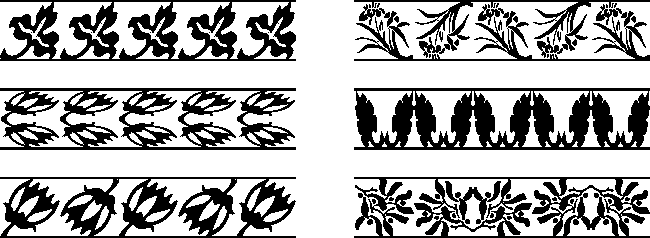
\includegraphics{../graphics/fpfrieze.pdf}
\end{center}
In each case, the pattern above can be thought of as an infinite strip
with the pattern continuing indefinitely.  Frieze patterns often have
symmetry in their structure. While in real-life, the symmetry would
not be perfect, it is useful in mathematics to simplify reality by
replacing the real patterns by idealized designs.  In this chapter, we
will study the symmetry of frieze patterns. At this point we will
refrain from giving a rigorous definition of a \textit{frieze
  pattern}. Instead, this will be a result of our work in this
chapter.


\break

\subsection{Symmetries}

\subsection*{Translations}\index{translation}

Perhaps the most apparent symmetry that frieze patters can exhibit is
symmetry through \textit{horizontal translations}:
\begin{center}

\includegraphics{../graphics/fptrans.pdf}
\end{center}
We will not only insist that a frieze pattern always have
translational symmetry, but we will also insist that such a
translation is \textit{discrete}, meaning that it occurs in distinct
``hops'' of some minimal distance. So, for example, the while the
following patterns have minimal discrete translations, 
\begin{center}

\includegraphics{../graphics/fptransDis.pdf}
\end{center}
this pattern
\begin{center}

\includegraphics{../graphics/fptransNot.pdf}
\end{center}
does not, and hence will not technically be considered a frieze
pattern. To be completely explicit: 
\begin{center}
\textbf{All frieze patterns have symmetry through a minimal discrete
  horizontal translation.}
\end{center}
\begin{dfn}\index{minimal cell}
A \textbf{minimal cell} is the smallest slice of a frieze
pattern that will produce the entire frieze pattern through horizontal
translations.
\end{dfn}

\begin{war}
The minimal cell of a frieze pattern is not unique! Consider
\begin{center}
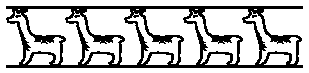
\includegraphics{../graphics/fptransMinEG.pdf}
\end{center}
both
\begin{center}
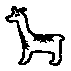
\includegraphics{../graphics/fptransMinEGCell.pdf} \qquad\text{and}\qquad  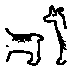
\includegraphics{../graphics/fptransMinEGCell2.pdf}
\end{center}
are minimal cells.
\end{war} 



\subsection*{Horizontal Reflections}\index{horizontal reflection}

Frieze patterns can have symmetry through \textit{horizontal reflections}:
\[

\includegraphics{../graphics/fphoriz.pdf}
\]
Some frieze patterns have symmetry through horizontal reflections, while
others don't.
\begin{ques} 
Can you identify the frieze patterns below with symmetry through
horizontal reflections?
\[
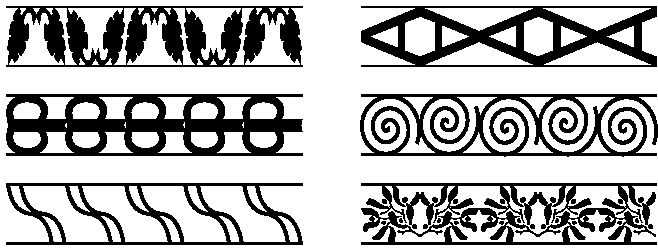
\includegraphics{../graphics/fpfriezeHoriz.pdf}
\]
\end{ques}

\begin{war}
Remember: A horizontal reflection reflects across a vertical line!
\end{war}



\subsection*{Vertical Reflections}\index{vertical reflection}


Frieze patterns can have symmetry through \textit{vertical reflections}:
\[

\includegraphics{../graphics/fpvertical.pdf}
\]

\begin{ques}
Can you identify the frieze patterns below with symmetry through
vertical reflections?
\[
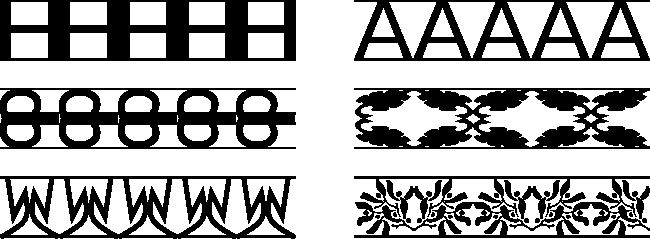
\includegraphics{../graphics/fpfriezeVert-Horiz.pdf}
\]
\end{ques}

\begin{war}
Remember: A vertical reflection reflects across a horizontal
line!
\end{war}




\subsection*{Glide Reflections}\index{glide reflection}

Frieze patterns can have symmetry through \textit{glide reflections}:
\[

\includegraphics{../graphics/fpglide.pdf}
\]

\begin{ques}
Can you identify the frieze patterns below with symmetry through glide
reflections?
\[
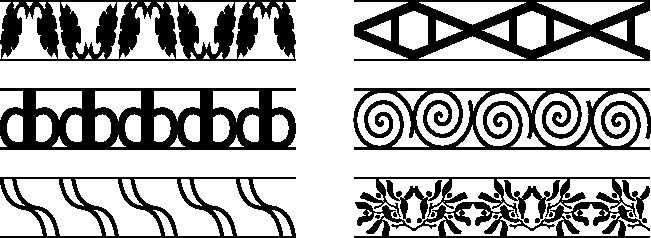
\includegraphics{../graphics/fpfriezeGlide.pdf}
\]
\end{ques}

\begin{ques}
If a frieze pattern has symmetry through translations and vertical
reflections, must it have symmetry through glide reflections?
\end{ques}
\QM




\subsection*{Rotations}\index{rotations}

Finally, frieze patterns can have symmetry through $180^\circ$
rotations.
\[
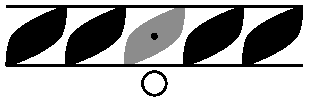
\includegraphics{../graphics/fprot.pdf}
\]

\begin{ques}
Can you identify the frieze patterns below that have symmetry through
$180^\circ$ rotations?
\[
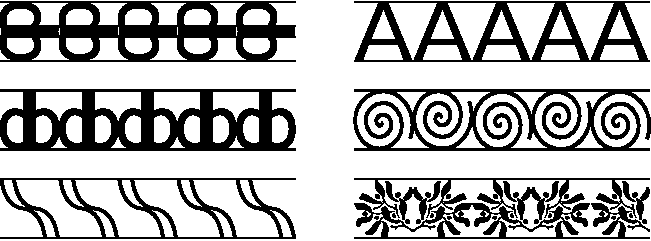
\includegraphics{../graphics/fpfriezeRot.pdf}
\]
\end{ques}

\begin{ques}
Suppose you have a frieze pattern with symmetry through both glide
reflections and $180^\circ$ rotations. Must this pattern also have
symmetry through horizontal reflections?
\end{ques}
\QM


\begin{ques}
Imagine that you have a frieze pattern that has symmetry through
horizontal reflections and $180^\circ$ rotations, but not through
vertical reflections. Could the center of the rotation be on the
vertical line that defines the reflection?
\end{ques}

I think I'll step in and give you a big hint. Consider the following
set of pictures and mysterious symbols:
\[
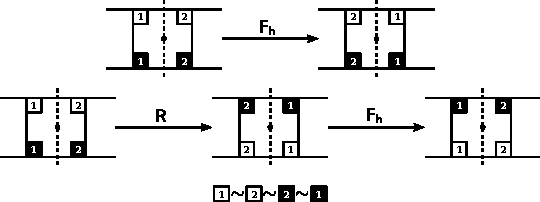
\includegraphics{../graphics/friezeRotRefCent.pdf}
\]
\begin{ques}
Can you explain what these pictures are trying to express?
\end{ques}
\QM


\newpage

\problems
\begin{enumerate}
\item Explain what it means for a frieze pattern to have symmetry
  through horizontal translations. Feel free to draw pictures to help out.
\item Explain what it means for a frieze pattern to have symmetry
  through horizontal reflections. Feel free to draw pictures to help out.
\item Explain what it means for a frieze pattern to have symmetry
  through vertical reflections. Feel free to draw pictures to help out.
\item Explain what it means for a frieze pattern to have symmetry
  through glide reflections. Feel free to draw pictures to help out.
\item Explain what it means for a frieze pattern to have symmetry
  through $180^\circ$ rotations. Feel free to draw pictures to help out.
\item Draw a frieze pattern that exhibits symmetry through horizontal
  translations and identify $3$ different minimal cells.
\item Draw a frieze pattern that exhibits symmetry through horizontal
  translations and glide reflections, but does not have symmetry
  through any other transformation. Be sure to identify a minimal
  cell.
\item Draw a frieze pattern that exhibits symmetry through horizontal
  translations and horizontal reflections, but does not have symmetry
  through any other transformation. Be sure to identify a minimal
  cell.
\item Draw a frieze pattern that exhibits symmetry through horizontal
  translations and $180^\circ$ rotations, but does not have symmetry
  through any other transformation. Be sure to identify a minimal
  cell.
\item Draw a frieze pattern that exhibits symmetry through horizontal
  translations, vertical reflections, and glide reflections, but does
  not have symmetry through any other transformation. Be sure to
  identify a minimal cell.
\item Draw a frieze pattern that exhibits symmetry through horizontal
  translations, horizontal reflections, glide reflections, and
  $180^\circ$ rotations, but does not have symmetry through any other
  transformation. Be sure to identify a minimal cell.
\item Draw a frieze pattern that exhibits symmetry through horizontal
  translations, horizontal reflections, vertical reflections, glide
  reflections, and $180^\circ$ rotations. Be sure to identify a
  minimal cell.
\item Consider the following frieze pattern:
\[
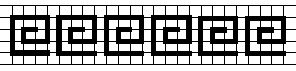
\includegraphics{../graphics/fpGraphEx1.pdf}
\]
Explicitly write down the matrices for the symmetries of this
pattern. Explain your reasoning.
\item Consider the following frieze pattern:
\[
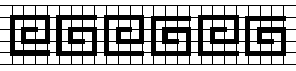
\includegraphics{../graphics/fpGraphEx2.pdf}
\]
Explicitly write down the matrices for the symmetries of this
pattern. Explain your reasoning.
\item Consider the following frieze pattern:
\[
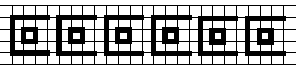
\includegraphics{../graphics/fpGraphEx3.pdf}
\]
Explicitly write down the matrices for the symmetries of this
pattern. Explain your reasoning.
\item Consider the following frieze pattern:
\[
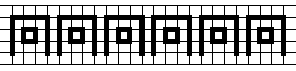
\includegraphics{../graphics/fpGraphEx4.pdf}
\]
Explicitly write down the matrices for the symmetries of this
pattern. Explain your reasoning.
\item Consider the following frieze pattern:
\[
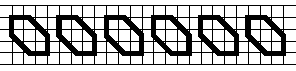
\includegraphics{../graphics/fpGraphEx5.pdf}
\]
Explicitly write down the matrices for the symmetries of this
pattern. Explain your reasoning.
\item Consider the following frieze pattern:
\[
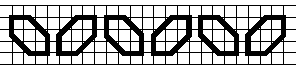
\includegraphics{../graphics/fpGraphEx6.pdf}
\]
Explicitly write down the matrices for the symmetries of this
pattern. Explain your reasoning.
\item Consider the following frieze pattern:
\[
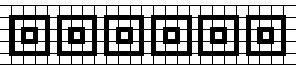
\includegraphics{../graphics/fpGraphEx7.pdf}
\]
Explicitly write down the matrices for the symmetries of this
pattern. Explain your reasoning.
\item Can you exhibit a frieze pattern with 
symmetry through $180^\circ$ rotations but not through glide reflections?
If so, present such a pattern and identify a minimal translation
cell. If not, explain why not.
\item Can you exhibit a frieze pattern with 
symmetry through horizontal reflections but not through glide reflections?
If so, present such a pattern and identify a minimal translation
cell. If not, explain why not.
\item Can you exhibit a frieze pattern with 
symmetry through vertical reflections but not through glide reflections?
If so, present such a pattern and identify a minimal translation
cell. If not, explain why not.
\item Can you exhibit a frieze pattern with 
symmetry through horizontal reflections and $180^\circ$ rotations but not through glide reflections?
If so, present such a pattern and identify a minimal translation
cell. If not, explain why not.


\end{enumerate}

\newpage







\section{Groups---Old and New}

\subsection{Old Friends}


We've already seen some groups. Now we're going to do something
that humans do really well, we're going to give them names.

\subsection*{Groups of Rotations}\index{rotation group}\index{R@$\R_\bullet$}

Consider any regular $n$-gon. We'll let $\R_n$ be the group of
rotations of this $n$-gon. As an example, consider $\R_3$. As we've seen
before, if we let $\mat{R} = \mat{R}_{120}$, then 
\[
\{\mat{I}, \mat{R}, \mat{R}^2\}
\]
forms a group. 

\begin{ques}
What are the elements of $\R_4$? What about $\R_n$?
\end{ques}
\QM

\subsection*{Groups of Reflections}\index{reflection group}\index{F@$\F_\bullet$}

Consider any regular $n$-gon. We'll let $\F_n$ be the group of all
reflections of this $n$-gon. So for a regular $3$-gon, we have
\[
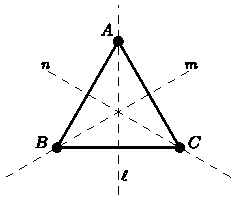
\includegraphics{../graphics/symTriRef.pdf}
\]
Let's write out the group table and see what we get, I've left it
mostly blank. By drawing some pictures, you can do this yourself
(seriously!):
\[
{
\renewcommand{\arraystretch}{1.5}
\begin{array}{| c || c | c | c |c | c | c |}
\hline
\circ & \mat{I} & \mat{F}_\l & \mat{F}_m  & \mat{F}_n & \mat{F}_\l \mat{F}_m &  \mat{F}_\l \mat{F}_n  \\ \hline \hline
\mat{I} &\rule[7mm]{13mm}{0mm} &\rule[7mm]{13mm}{0mm} &\rule[7mm]{13mm}{0mm} &\rule[7mm]{13mm}{0mm} &\rule[7mm]{13mm}{0mm} &  \rule[7mm]{13mm}{0mm}\\ \hline
\mat{F}_\l &\rule[7mm]{13mm}{0mm} & & & & &  \\ \hline
\mat{F}_m &\rule[7mm]{13mm}{0mm} & & & & &  \\ \hline
\mat{F}_n &\rule[7mm]{13mm}{0mm} & & & & &  \\ \hline
\mat{F}_\l\mat{F}_m &\rule[7mm]{13mm}{0mm} & & & & &  \\ \hline
\mat{F}_\l\mat{F}_n &\rule[7mm]{13mm}{0mm} & & & & &  \\ \hline
\end{array}}
\]

Checking with the definition of a group, we see that 
\[
\F_3 = \{ \mat{I}, \mat{F}_\l, \mat{F}_m, \mat{F}_n, \mat{F}_\l\mat{F}_m,\mat{F}_\l\mat{F}_n\}
\]
is indeed a group!

\begin{ques}
How many elements does $\F_n$ have?
\end{ques}
\QM



\subsection*{Symmetry Groups}

We have a special name for the complete symmetry group of a regular
$n$-gon:

\begin{dfn} The \textbf{dihedral group}\index{dihedral
  group}, denoted $\D_n$, is the group of symmetries of a regular
  $n$-gon.
\end{dfn}

\begin{ques}
How many symmetries does a regular $n$-gon have?
\end{ques}
\QM




\subsection{New Friends}


Not only can we make groups from the symmetries of regular $n$-gons,
but we can also make group tables from the symmetries of frieze
patterns. These groups are called \textit{frieze groups}.\index{frieze group}


\subsection*{The Groups $\boldsymbol{\Zt}$ and $\boldsymbol{\Zg}$}

The symmetries of the following frieze pattern form the group $\Zt$:\index{ZT@$\Zt$}
\[
\text{\huge $\Zt$:}\qquad\begin{array}{c}
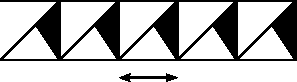
\includegraphics{../graphics/fptransGP.pdf}
\end{array}
\]
This pattern only has symmetry through horizontal translations. Let
$\mat{T}$ represent a translation of the minimal cell to the
right. Then $\mat{T}^{-1}$ is a translation of the minimal cell to the
left. From this we see that
\[
\mat{T}\mat{T}^{-1} = \mat{I}.
\]
Since frieze patterns are thought of as infinite strips, we can apply
a translation successively to itself an infinite number of times---and
each time it will represent a different symmetry of the frieze
pattern. The upshot of this is that a group of symmetries of a frieze
pattern will always have an infinite number of elements. Hence, the
group table will also be infinite. We'll denote this with ``$\cdots$''
in the table so we (meaning you!) can start to write out the partial
group table. Let's do it:
\[
{
\renewcommand{\arraystretch}{1.5}
\begin{array}{| c || c | c | c |c | c | c | c|}
\hline
\circ & \cdots & \mat{T}^{-2} & \mat{T}^{-1}  & \mat{I} & \mat{T} &  \mat{T}^2  & \cdots \\ \hline \hline
\cdots &\cdots & \cdots & \cdots  & \cdots & \cdots &  \cdots &  \cdots\\ \hline
\mat{T}^{-2} & \cdots &\rule[7mm]{13mm}{0mm} &\rule[7mm]{13mm}{0mm} &\rule[7mm]{13mm}{0mm} &\rule[7mm]{13mm}{0mm} &  \rule[7mm]{13mm}{0mm} &  \cdots\\ \hline
\mat{T}^{-1} & \cdots &\rule[7mm]{13mm}{0mm} & & & & & \cdots \\ \hline
\mat{I} & \cdots &\rule[7mm]{13mm}{0mm} & & & & & \cdots \\ \hline
\mat{T} & \cdots &\rule[7mm]{13mm}{0mm} & & & & & \cdots \\ \hline
\mat{T}^2 & \cdots &\rule[7mm]{13mm}{0mm} & & & & & \cdots \\ \hline
\cdots & \cdots & \cdots  &\cdots &\cdots &\cdots &\cdots & \cdots \\ \hline
\end{array}}
\]
Hence:
\[
\Zt = \{\dots, \mat{T}^{-3}, \mat{T}^{-2},\mat{T}^{-1}, \mat{I}, \mat{T},\mat{T}^2,\mat{T}^3, \dots\}
\]


The symmetries of the following frieze pattern form the group $\Zg$:\index{ZG@$\Zg$}
\[
\text{\huge $\Zg$:}\qquad\begin{array}{c}
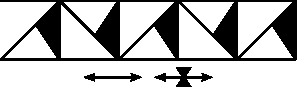
\includegraphics{../graphics/fpglideGP.pdf}
\end{array}
\]
This pattern only has symmetry through horizontal translations and
glide reflections. However, a minimal cell for this frieze pattern is
\[

\includegraphics{../graphics/fpglideMinTransCell.pdf}
\]
We'll let $\mat{T}$ represent the minimal translation of this cell to the
right. On the other hand, a smaller piece of the frieze pattern will
generate the entire pattern through glide reflections.  If we let
$\mat{G}$ represent this glide reflection to the right, we see that
\[
\mat{G}\mat{G}^{-1} = \mat{I} \qquad\text{and}\qquad\mat{G}\mat{G} = \mat{T}.
\]
So we (meaning you!) can start to write out the partial group table:
\[
{
\renewcommand{\arraystretch}{1.5}
\begin{array}{| c || c | c | c |c | c | c | c|}
\hline
\circ & \cdots & \mat{G}^{-2} & \mat{G}^{-1}  & \mat{I} & \mat{G} &  \mat{G}^2  & \cdots \\ \hline \hline
\cdots &\cdots & \cdots & \cdots  & \cdots & \cdots &  \cdots &  \cdots\\ \hline
\mat{G}^{-2} & \cdots &\rule[7mm]{13mm}{0mm} &\rule[7mm]{13mm}{0mm} &\rule[7mm]{13mm}{0mm} &\rule[7mm]{13mm}{0mm} &  \rule[7mm]{13mm}{0mm} &  \cdots\\ \hline
\mat{G}^{-1} & \cdots &\rule[7mm]{13mm}{0mm} & & & & & \cdots \\ \hline
\mat{I} & \cdots &\rule[7mm]{13mm}{0mm} & & & & & \cdots \\ \hline
\mat{G} & \cdots &\rule[7mm]{13mm}{0mm} & & & & & \cdots \\ \hline
\mat{G}^2 & \cdots &\rule[7mm]{13mm}{0mm} & & & & & \cdots \\ \hline
\cdots & \cdots & \cdots  &\cdots &\cdots &\cdots &\cdots & \cdots \\ \hline
\end{array}}
\]
We'll denote this group by:
\[
\Zg = \{\dots, \mat{G}^{-3}, \mat{G}^{-2},\mat{G}^{-1}, \mat{I}, \mat{G},\mat{G}^2,\mat{G}^3, \dots\}
\]


\begin{ques}
What is the connection between the group tables for $\Zt$ and $\Zg$?
\end{ques}
\QM







\subsection*{The Group $\boldsymbol{\Zgf}$}

The symmetries of the following frieze pattern form the group $\Zgf$:\index{ZGF@$\Zgf$}
\[
\text{\huge $\Zgf$:}\qquad\begin{array}{c}

\includegraphics{../graphics/fpverticalGP.pdf}
\end{array}
\]
This pattern only has symmetry through horizontal translations, glide
reflections, and vertical reflections. Let $\mat{T}$ be the horizontal
translation, $\mat{G}$ be the glide reflection, and $\mat{F}$ be the
vertical reflection.

\begin{eg} 
Can you express $\mat{T}$ entirely in terms of $\mat{F}$ and
$\mat{G}$?

Check out these pictures:
\[
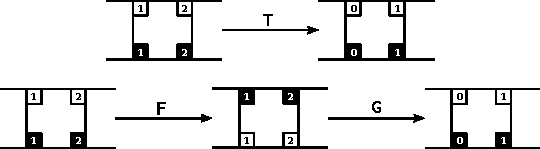
\includegraphics{../graphics/friezeGF-T.pdf}
\]
The first line shows us a translation. The second line shows us
$\mat{G}\mat{F}$. Since they are the same, we've expressed $\mat{T}$
entirely in terms of $\mat{F}$ and $\mat{G}$.
\end{eg}


\begin{ques} Is $\mat{G}\mat{F} = \mat{F}\mat{G}$?
\end{ques}
\QM

\begin{ques}
An arbitrary element of $\Zt$ looks like $\mat{T}^n$. An arbitrary
element of $\Zg$ looks like $\mat{G}^n$. What does an arbitrary element
of $\Zgf$ look like?
\end{ques}
\QM

\begin{eg}
Explain how we know $\Zgf$ is a group.

To do this, we need to check the four parts of the definition of a
group:
\begin{enumerate}
\item Since all of our elements are matrices, and matrix multiplication is associative, we have the needed ``associative operation.''
\item Since $\Zgf$ is the list of all of the symmetries of the frieze
  pattern above, it is necessarily closed under our operation.
\item The identity element $\mat{I}$ is simply the symmetry that
  ``does nothing.''
\item Every element has an inverse, because every transformation can
  be undone.
\end{enumerate}
So $\Zgf$ is a group!
\end{eg}





\subsection*{The Groups $\boldsymbol{\Ztf}$, $\boldsymbol{\Ztr}$, and $\boldsymbol{\Zgr}$}


The symmetries of the following frieze pattern form the group
$\Ztf$:\index{ZTF@$\Ztf$}
\[
\text{\huge $\Ztf$:}\qquad\begin{array}{c}

\includegraphics{../graphics/fphorizGP.pdf}
\end{array}
\]
This pattern only has symmetry through horizontal translations and
horizontal reflections. Let $\mat{T}$ be the horizontal translation
and $\mat{F}$ be the horizontal reflection.

\begin{ques} Is $\mat{T}\mat{F} = \mat{F}\mat{T}$?
\end{ques}
\QM

Once again, we (meaning you!) can start to write out the partial group
table:


\[
{
\renewcommand{\arraystretch}{1.5}
\begin{array}{| c || c | c | c | c | c | c | c | c | c | c|}
\hline
\circ & \cdots & \mat{T}^{-2} & \mat{T}^{-1}\mat{F}  & \mat{T}^{-1} & \mat{I} & \mat{T} &  \mat{F} & \mat{T} \mat{F} & \mat{T}^2  & \cdots \\ \hline \hline
\cdots &\cdots & \cdots & \cdots  & \cdots & \cdots &  \cdots  & \cdots & \cdots &  \cdots &  \cdots\\ \hline
\mat{T}^{-2} & \cdots &\rule[7mm]{13mm}{0mm} &\rule[7mm]{13mm}{0mm} &\rule[7mm]{13mm}{0mm} &\rule[7mm]{13mm}{0mm}  &\rule[7mm]{13mm}{0mm} &\rule[7mm]{13mm}{0mm} &\rule[7mm]{13mm}{0mm} &  \rule[7mm]{13mm}{0mm} &  \cdots\\ \hline
\mat{T}^{-1} \mat{F} & \cdots &\rule[7mm]{13mm}{0mm} & & & & & & & & \cdots \\ \hline
\mat{T}^{-1} & \cdots &\rule[7mm]{13mm}{0mm} & & & & & & & & \cdots \\ \hline
\mat{I} & \cdots &\rule[7mm]{13mm}{0mm} & & & & & & & &\cdots \\ \hline
\mat{T} & \cdots &\rule[7mm]{13mm}{0mm} & & & & & & & & \cdots \\ \hline
\mat{F} & \cdots &\rule[7mm]{13mm}{0mm} & & & & & & & & \cdots \\ \hline
\mat{T} \mat{F} & \cdots &\rule[7mm]{13mm}{0mm} & & & & & & & & \cdots \\ \hline
\mat{T}^2 & \cdots &\rule[7mm]{13mm}{0mm} & & & & & & & &\cdots \\ \hline
\cdots & \cdots & \cdots  &\cdots &\cdots &\cdots &\cdots & \cdots &\cdots &\cdots & \cdots \\ \hline
\end{array}}
\]

\begin{ques}
An arbitrary element of $\Zt$ looks like $\mat{T}^n$. An arbitrary
element of $\Zg$ looks like $\mat{G}^n$. What does an arbitrary element
of $\Ztf$ look like?
\end{ques}
\QM










The symmetries of the following frieze pattern form the group $\Ztr$:\index{ZTR@$\Ztr$}
\[
\text{\huge $\Ztr$:}\qquad\begin{array}{c}

\includegraphics{../graphics/fprotGP.pdf}
\end{array}
\]
This pattern only has symmetry through horizontal translations and
$180^\circ$ rotations. Let $\mat{T}$ be the horizontal translation and
$\mat{R}$ be the $180^\circ$ rotation.

\begin{ques} Is $\mat{T}\mat{R} = \mat{R}\mat{T}$?
\end{ques}
\QM

\begin{ques}
Can you remind us why this is a group?
\end{ques}
\QM

\begin{ques}
An arbitrary element of $\Zt$ looks like $\mat{T}^n$. An arbitrary
element of $\Zg$ looks like $\mat{G}^n$. What does an arbitrary element
of $\Ztr$ look like?
\end{ques}
\QM










The symmetries of the following frieze pattern form the group
$\Zgr$:\index{ZGR@$\Zgr$}
\[
\text{\huge $\Zgr$:}\qquad\begin{array}{c}
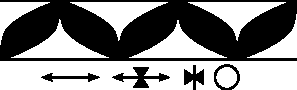
\includegraphics{../graphics/fpzgrGP.pdf}
\end{array}
\]
This pattern only has symmetry through horizontal translations, glide
reflections, horizontal reflections, and $180^\circ$ rotations. Let
$\mat{T}$ be the horizontal translation, $\mat{G}$ be the glide
reflection, $\mat{F}$ be the horizontal reflection, and $\mat{R}$ be
the $180^\circ$ rotation.

\begin{ques} 
Can you express $\mat{T}$ and $\mat{F}$ entirely in terms of $\mat{G}$
and $\mat{R}$?
\end{ques}
\QM
\begin{ques} Is $\mat{G}\mat{R} = \mat{R}\mat{G}$?
\end{ques}
\QM

\begin{ques}
What's the group table of $\Zgr$ going to look like?
\end{ques}
\QM


\begin{ques}
An arbitrary element of $\Zt$ looks like $\mat{T}^n$. An arbitrary
element of $\Zg$ looks like $\mat{G}^n$. What does an arbitrary element
of $\Zgr$ look like?
\end{ques}
\QM









\subsection*{The Group $\boldsymbol{\Ztfr}$}

The symmetries of the following frieze pattern form the group $\Ztfr$:\index{ZTRF@$\Ztfr$}
\[
\text{\huge $\Ztfr$:}\qquad\begin{array}{c}
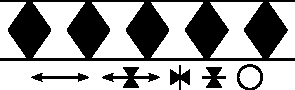
\includegraphics{../graphics/fptfrGP.pdf}
\end{array}
\]
This pattern has symmetry through horizontal translations, glide
reflections, horizontal reflections, vertical reflections and
$180^\circ$ rotations.  Let $\mat{T}$ be the horizontal translation,
$\mat{G}$ be the glide reflection, $\mat{F_h}$ be the horizontal
reflection, $\mat{F_v}$ be the vertical reflection, and $\mat{R}$ be
the $180^\circ$ rotation.


\begin{ques} 
Can you express $\mat{G}$ and $\mat{F_h}$ entirely in terms of $\mat{T}$, $\mat{F_v}$, and $\mat{R}$?
\end{ques}
\QM
\begin{ques} 
Is $\mat{T}\mat{F_v} = \mat{F_v}\mat{T}$? What about $\mat{T}\mat{R} =
\mat{R}\mat{T}$? What about $\mat{F_v}\mat{R} = \mat{R}\mat{F_v}$?
\end{ques}
\QM

Let's start to write out the partial group table:
\[
{
\renewcommand{\arraystretch}{1.5}
\begin{array}{| c || c | c | c | c | c | c | c | c | c | c | c | c|}
\hline
\circ & \cdots & \mat{T}^{-1}\mat{R} & \mat{T}^{-1}\mat{F}  & \mat{T}^{-1} & \mat{I} & \mat{T} &  \mat{F} & \mat{R} & \mat{T}\mat{F} & \mat{T}\mat{R} & \mat{F} \mat{R}  & \cdots \\ \hline \hline
\cdots &\cdots & \cdots & \cdots  & \cdots & \cdots &  \cdots  & \cdots & \cdots &  \cdots &  \cdots &  \cdots &  \cdots\\ \hline
\mat{T}^{-1}\mat{R} & \cdots &\rule[7mm]{8mm}{0mm} &\rule[7mm]{8mm}{0mm} &\rule[7mm]{8mm}{0mm} &\rule[7mm]{8mm}{0mm}  &\rule[7mm]{8mm}{0mm} &\rule[7mm]{8mm}{0mm} &\rule[7mm]{8mm}{0mm} &  \rule[7mm]{8mm}{0mm} &\rule[7mm]{8mm}{0mm} &  \rule[7mm]{8mm}{0mm} &  \cdots\\ \hline
\mat{T}^{-1} \mat{F} & \cdots &\rule[7mm]{8mm}{0mm} & & & & & & & & & & \cdots \\ \hline
\mat{T}^{-1} & \cdots &\rule[7mm]{8mm}{0mm} & & & & & & & & & & \cdots \\ \hline
\mat{I} & \cdots &\rule[7mm]{8mm}{0mm} & & & & & & & & & & \cdots \\ \hline
\mat{T} & \cdots &\rule[7mm]{8mm}{0mm} & & & & & & & & & & \cdots \\ \hline
\mat{F} & \cdots &\rule[7mm]{8mm}{0mm} & & & & & & & & & & \cdots \\ \hline
\mat{R} & \cdots &\rule[7mm]{8mm}{0mm} & & & & & & & & & & \cdots \\ \hline
\mat{T} \mat{F} & \cdots &\rule[7mm]{8mm}{0mm} & & & & & & & & & & \cdots \\ \hline
\mat{T} \mat{R} & \cdots &\rule[7mm]{8mm}{0mm} & & & & & & & & & & \cdots \\ \hline
\mat{F} \mat{R} & \cdots &\rule[7mm]{8mm}{0mm} & & & & & & & & & & \cdots \\ \hline
\cdots & \cdots & \cdots  &\cdots &\cdots &\cdots &\cdots & \cdots &\cdots &\cdots & \cdots &\cdots & \cdots \\ \hline
\end{array}}
\]


\begin{ques}
An arbitrary element of $\Zt$ looks like $\mat{T}^n$. An arbitrary
element of $\Zg$ looks like $\mat{G}^n$. What does an arbitrary element
of $\Ztfr$ look like?
\end{ques}
\QM
\vfill
\break



\paragraph{Some Observations and Thoughts}


Look back at the partial group tables that you have constructed. What
patterns do you notice? Which group tables are fundamentally the same?
Which are different? If we expanded the partial group tables even
more, could you continue to fill them out?



As a gesture of friendship, here is a collection of the frieze groups
along with frieze patterns:
\[
{
\renewcommand{\arraystretch}{4}
\begin{array}{c}
\text{\huge $\Zt$:}\qquad\begin{array}{c}
\includegraphics{../graphics/fptransGP.pdf}
\end{array}\\
\text{\huge $\Zg$:}\qquad\begin{array}{c}
\includegraphics{../graphics/fpglideGP.pdf}
\end{array}\\
\text{\huge $\Zgf$:}\qquad\begin{array}{c}
\includegraphics{../graphics/fpverticalGP.pdf}
\end{array}\\
\text{\huge $\Ztf$:}\qquad\begin{array}{c}
\includegraphics{../graphics/fphorizGP.pdf}
\end{array}\\
\text{\huge $\Ztr$:}\qquad\begin{array}{c}
\includegraphics{../graphics/fprotGP.pdf}
\end{array}\\
\text{\huge $\Zgr$:}\qquad\begin{array}{c}
\includegraphics{../graphics/fpzgrGP.pdf}
\end{array}\\
\text{\huge $\Ztfr$:}\qquad\begin{array}{c}
\includegraphics{../graphics/fptfrGP.pdf}
\end{array}
\end{array}
}
\]



\newpage

\problems
\begin{enumerate}
\item State the definition of a group of matrices.
\item Explain what is meant by the symbol $\R_n$. Give an example.
\item If a regular 2-gon is just a line segment, give the group table
  for $\R_2$.
\item Give the group table for $\R_3$.
\item Give the group table for $\R_4$.
\item Give the group table for $\R_5$.
\item How many elements does $\R_n$ have? Explain your reasoning.
\item Explain what is meant by the symbol $\F_n$. Given an example. 
\item If a regular 2-gon is just a line segment, give the group table
  for $\F_2$.
\item Give the group table for $\F_3$.
\item Give the group table for $\F_4$.
\item Give the group table for $\F_5$.
\item How many elements does $\F_n$ have? Explain your reasoning.
\item Explain what is meant by the symbol $\D_n$. Given an example.
\item If a regular 2-gon is just a line segment, give the group table
  for $\D_2$.
\item Give the group table for $\D_3$.
\item Give the group table for $\D_4$.
\item Give the group table for $\D_5$.
\item How many elements does $\D_n$ have? Explain your reasoning.
\item Draw three different frieze patterns whose symmetries are
  described by $\Zt$.
\item Draw three different frieze patterns whose symmetries are
  described by $\Zg$.
\item Draw three different frieze patterns whose symmetries are
  described by $\Zgf$.
\item Draw three different frieze patterns whose symmetries are
  described by $\Ztf$.
\item Draw three different frieze patterns whose symmetries are
  described by $\Ztr$.
\item Draw three different frieze patterns whose symmetries are
  described by $\Zgr$.
\item Draw three different frieze patterns whose symmetries are
  described by $\Ztfr$.
%\item SOMETHING WITH LATTICE DIAGRAMS

\end{enumerate}

\newpage



\section{There Can Be Only Seven}


The title of this section says it all---there are only seven frieze
groups. Believe it or not, we will tackle this monster by solving an
unrelated problem!

\subsection{Pascal's Pizza Shop}

\textit{Pascal's Pizza Shop} makes a variety of pizzas, all which come
with cheese.  However, they do not offer double toppings---no ``double
cheese'' and so on.

\begin{ques}
If he offers two additional toppings, namely basil and garlic.
\begin{enumerate}
\item How many different 1-item pizzas (cheese plus one other
  topping) can he make?  List the possibilities.
\item How many different 2-item pizzas can he make?  List them.
\item How many different 0-item pizzas can he make?
\item In total, how many different pizzas can he make?
\end{enumerate}
\end{ques}
\QM

\begin{ques}
Now suppose he has basil, garlic, and spinach toppings
available.
\begin{enumerate}
\item How many 0-item pizzas can he make?
\item How many 1-item pizzas can he make?
\item How many 2-item pizzas can he make?
\item How many 3-item pizzas can he make?
\item In total, how many different pizzas can he make?
\end{enumerate}
\end{ques}
\QM

\begin{ques}
Complete the following chart by listing and counting the
possibilities, where $n$ is the number of toppings Pascal has
available, and $k$ is the number of toppings used.\\
\[
{\renewcommand{\arraystretch}{2}
\begin{array}{|c||c|c|c|c|c|c||c|}
    \hline
          & k=0 & k=1 & k=2 & k=3 & k=4 & k=5 & \text{Total}\\
    \hline\hline
    n=0 &       &       &       &       &       &    &  \\
    \hline
    n=1 &       &       &       &       &       &    &  \\
    \hline
    n=2 &       &       &       &       &       &    &  \\
    \hline
    n=3 &       &       &       &       &       &    &  \\
    \hline
    n=4 &       &       &       &       &       &    &  \\
    \hline
    n=5 &       &       &       &       &       &    &  \\
    \hline
\end{array}}
\]
\end{ques}
\QM

\begin{ques} 
Often the numbers in the table you filled in above are arranged a bit
differently, as below, where the top ``1" counts the number of
0-topping pizzas that can be made if zero toppings are
available. Complete the first 8 rows of the triangle, which is called
\textit{Pascal's Triangle}.\index{Pascal's Triangle}
\[
\begin{tabular}{c c c c c c c}
      &   &   & 1 &   &   &  \\
      &   & 1 &   & 1 &   &  \\
      & 1 &   & 2 &   & 1 &  \\
    1 &   & 3 &   & 3 &   & 1
\end{tabular}
\vspace{2in}
\]
Do you see some patterns in the triangle?  Describe them and try to
explain why (in terms of pizzas) why they occur.
\end{ques}
\QM



\subsection{Symmetries as Toppings}

We are going to count the various way that a frieze pattern could have
symmetry. Let's list the basic geometric transformations that can
preserve frieze patterns:
\begin{enumerate}
\item Horizontal translations denoted by $\mat{T}$.
\item Horizontal reflections denoted by $\mat{F_h}$.
\item Vertical reflections denoted by $\mat{F_v}$.
\item Glide reflections denoted by $\mat{G}$.
\item Rotations of $180^\circ$ denoted by $\mat{R}$.
\end{enumerate}
Hence, just as we counted pizza's with a number of toppings, we can
count groups of symmetries, where we select groups containing the
transformations above.

To start, not that every frieze pattern has symmetry through horizontal
translations. So we don't need to count that one---this is like saying
that every pizza has cheese on it. Let's list out all possible combinations
of the remaining 4 transformations. To make sure we get them all, we are
going to do this in a very orderly fashion.

\begin{ques} 
How many combinations of symmetries should there be with a single
transformation?  What are they?
\end{ques}
\QM

\begin{ques} 
How many combinations of symmetries should there be with two
transformations?  What are they?
\end{ques}
\QM

\begin{ques} 
How many combinations of symmetries should there be with three
transformations?  What are they?
\end{ques}
\QM

\begin{ques} 
How many combinations of symmetries should there be with four
transformations?  What are they?
\end{ques}
\QM



\subsection{Grouping by Groups}

Now that you have a listing of all possible combinations of the
symmetries of the frieze patterns, let's literally try to group them
by groups---we're going to put the combinations you already found into
the groups we already know. Here are two leading questions to help you
out:


\begin{ques} 
Why must a frieze pattern have symmetry through glide reflections, if
you know it has symmetry through both translations and vertical
reflections?
\end{ques}

I'll take this one, just to show you how it's done. We'll imagine some
sort of generic frieze pattern, and draw the following pictures:
\[
\includegraphics{../graphics/friezeTF-G.pdf}
\]
Hence, from the picture we see that if the frieze pattern has symmetry
through both $\mat{T}$ and $\mat{F_v}$, then it must also have
symmetry through $\mat{G}$.


\begin{ques} 
Why must a frieze pattern have symmetry through $180^\circ$ rotations,
if you know it has symmetry through translations, glide reflections,
and horizontal reflections?
\end{ques}
\QM


\begin{ques} 
Why must a frieze pattern have symmetry through glide reflections, if
you know it has symmetry through translations, horizontal reflections,
and $180^\circ$ rotations?
\end{ques}
\QM

\begin{ques} 
Why must a frieze pattern have symmetry through glide reflections, if
you know it has symmetry through translations, horizontal reflections,
and vertical reflections?
\end{ques}
\QM

\begin{ques} 
Why must a frieze pattern have symmetry through $180^\circ$ rotations, if
you know it has symmetry through translations, horizontal reflections,
and vertical reflections?
\end{ques}
\QM


\begin{ques} 
Why must a frieze pattern have symmetry through vertical reflections,
if you know it has symmetry through translations, horizontal
reflections, and $180^\circ$ rotations?
\end{ques}
\QM




\begin{ques} 
Can you figure out which frieze groups go with which collections of
symmetries you listed above?
\end{ques}
\QM


From this we can finally give a rigorous definition of a frieze pattern
as promised:

\begin{dfn}\index{frieze pattern}
A \textbf{frieze pattern} is a pattern whose symmetries are given by
one of the seven frieze groups.
\end{dfn}




\paragraph{Some Observations and Thoughts}


Now that we have classified all of the frieze groups, let me tell you about
another classification project. Around 1971, a mathematician by the
name of Gorenstein sought to understand \textbf{all} finite
groups. To do this, he proposed that we attempt to classify all of
what are called ``finite simple groups.'' While the definition of a
\textit{simple group} is somewhat beyond the scope of this course, to
put it in SAT terms:
\begin{center}
\textit{simple group} is to \textit{group} \qquad as \qquad \textit{prime number} is to \textit{number}
\end{center}
This goal was eventually finished in 2004---however, the proof of the
classification was enormous. It spanned 15000 pages and required the
work of over 100 mathematicians. Some of the arguments are described
as ``diabolically difficult'' and the proof surely presses to the
limits of human thought.







\newpage

\problems
\begin{enumerate}
\item Suppose you have two toppings, namely basil and garlic.
\begin{enumerate}
\item How many different 0-item pizzas (cheese pizzas) can you make?
\item How many different 1-item pizzas (cheese plus one other topping)
  can you make?  List the possibilities.
\item How many different 2-item pizzas can you make?  List the
  possibilities.
\item In total, how many different pizzas can you  make?
\end{enumerate}
Explain your reasoning.
\item Suppose you have three toppings, namely basil, garlic, and spinach.
\begin{enumerate}
\item How many different 0-item pizzas (cheese pizzas) can you make?
\item How many different 1-item pizzas (cheese plus one other
  topping) can you make?  List the possibilities.
\item How many different 2-item pizzas can you make?  List the
  possibilities.
\item How many different 3-item pizzas can you make?  List the
  possibilities.
\item In total, how many different pizzas can you  make?
\end{enumerate}
Explain your reasoning.
\item Suppose you have four toppings, namely basil, garlic, spinach,
  and tomatoes.
\begin{enumerate}
\item How many different 0-item pizzas (cheese pizzas) can you make?
\item How many different 1-item pizzas (cheese plus one other
  topping) can you make?  List the possibilities.
\item How many different 2-item pizzas can you make?  List the
  possibilities.
\item How many different 3-item pizzas can you make?  List the
  possibilities.
\item How many different 4-item pizzas can you make?  List the
  possibilities.
\item In total, how many different pizzas can you  make?
\end{enumerate}
Explain your reasoning.
\item Write down the first $8$ rows of Pascal's Triangle. Explain what
  each entry means in terms of pizzas and toppings.
\item Describe how to get a new row of Pascal's Triangle from the
  previous row. 
\item Explain in terms of pizzas and toppings why the method described
  in the solution to the previous exercise works.
\item Describe how to find the total number of pizzas one can make
  given a number of toppings.
\item Explain in terms of pizzas and toppings why the method described
  in the solution to the previous exercise works.
\item List the possible symmetries of frieze patterns and give a brief
  explanation of each.
\item How many combinations of symmetries of frieze patterns should
  there be with a single transformation?  What are they? Explain your reasoning.
\item How many combinations of symmetries of frieze patterns should
  there be with two transformations?  What are they? Explain your
  reasoning.
\item How many combinations of symmetries of frieze patterns should
  there be with three transformations?  What are they? Explain your
  reasoning.
\item How many combinations of symmetries of frieze patterns should
  there be with four transformations?  What are they? Explain your
  reasoning.
\item Why must a frieze pattern have symmetry through glide
  reflections, if you know it has symmetry through both translations
  and vertical reflections?
\item Why must a frieze pattern have symmetry through $180^\circ$
  rotations, if you know it has symmetry through translations, glide
  reflections, and horizontal reflections?
\item Why must a frieze pattern have symmetry through glide
  reflections, if you know it has symmetry through translations,
  horizontal reflections, and $180^\circ$ rotations?
\item Why must a frieze pattern have symmetry through glide
  reflections, if you know it has symmetry through translations,
  horizontal reflections, and vertical reflections?
\item Why must a frieze pattern have symmetry through $180^\circ$
  rotations, if you know it has symmetry through translations,
  horizontal reflections, and vertical reflections?
\item Why must a frieze pattern have symmetry through vertical
  reflections, if you know it has symmetry through translations,
  horizontal reflections, and $180^\circ$ rotations?
\item Give three different pictures whose symmetries are described by
  $\R_3$.
\item Give three different pictures whose symmetries are described by
  $\R_4$.
\item Give three different pictures whose symmetries are described by
  $\D_3$.
\item Give three different pictures whose symmetries are described by
  $\D_4$.
\item Consider the simplest frieze group $\Zt$. Can you give a
  pattern that doesn't really resemble a frieze pattern whose
  symmetries are described by this group?
\end{enumerate}

\chapter{Folding and Tracing Constructions}
\begin{quote} 
We don't even know if Foldspace introduces us to one universe or
many\dots

\hfill---Frank Herbert
\end{quote}

\section{Constructions}

While origami as an art form is quite ancient, folding and tracing constructions
in mathematics are relatively new. The earliest mathematical
discussion of folding and tracing constructions that I know of appears in
T.\ Sundara Row's book \textit{Geometric Exercises in Paper Folding},
\cite{row}, first published near the end of the Nineteenth Century. In
the Twentieth Century it was shown that every construction that is
possible with a compass and straightedge can be done with
folding and tracing. Moreover, there are constructions that are possible via
folding and tracing that are \textit{impossible} with compass and straightedge
alone. This may seem strange as you can draw a circle with a compass,
yet this seems impossible to do via paper-folding. We will address
this issue in due time. Let's get down to business---here are the
rules of folding and tracing constructions:


\subsubsection*{Rules for Folding and Tracing Constructions}
\begin{enumerate}
\item You may only use folds, a marker, and semi-transparent paper.
\item Points can only be placed in two ways:
\begin{enumerate}
\item As the intersection of two lines. 
\item By marking ``through'' folded paper onto a previously placed
  point. Think of this as when the ink from a permanent marker
  ``bleeds'' through the paper.
\end{enumerate}
\item Lines can only be obtained in three ways:
\begin{enumerate}
\item By joining two points---either with a drawn line or a fold.
\item As a crease created by a fold. 
\item By marking ``through'' folded paper onto a previously placed
  line.
\end{enumerate}
\item One can only fold the paper when:
\begin{enumerate}
\item Matching up points with points.
\item Matching up a line with a line.
\item Matching up two points with two intersecting lines.
\end{enumerate}
\end{enumerate}


Now we are going to present several basic constructions. We will
proceed by the order of difficulty of the construction.


\begin{con}[Transferring a Segment]\index{folding and tracing!transferring a segment}  
Given a segment, we wish to move it so that it starts on a given
point, on a given line.
\end{con}


\begin{con}[Copying an Angle]\index{folding and tracing!copying an angle} 
Given a point on a line and some angle, we wish to copy the given
angle so that the new angle has the point as its vertex and the line
as one of its edges.
\end{con}

Transferring segments and copying angles using folding and tracing without a
``bleeding marker'' can be tedious. Here is an easy way to do it: 
\begin{center}
\textbf{Use 2 sheets of paper and a pen that will mark through multiple
sheets.}
\end{center}

\begin{ques} 
Can you find a way to do the above constructions without using a
marker whose ink will pass through paper?
\end{ques}
\QM

\begin{con}[Bisecting a Segment]\index{folding and tracing!bisecting a segment} 
Given a segment, we wish to cut it in half.
\begin{enumerate}
\item Fold the paper so that the endpoints of the segment meet.
\item The crease will bisect the given segment.
\end{enumerate}
\[
\includegraphics{../graphics/origamiBisect.pdf}
\]
\end{con}

\begin{ques} 
Which rule for folding and tracing constructions are we using above?
\end{ques}
\QM


\begin{con}[Perpendicular through a Point]\index{folding and tracing!perpendicular through a point}  
Given a point and a line, we wish to construct a line perpendicular to
the original line that passes through the given point.
\begin{enumerate}
\item Fold the given line onto itself so that the crease passes though
  the given point.
\item The crease will be the perpendicular line.
\end{enumerate}
\[
\includegraphics{../graphics/origamiPerpPoint.pdf}
\]
\end{con}

\begin{ques} Which rule for folding and tracing constructions are we using above?
\end{ques}
\QM




\begin{con}[Bisecting an Angle]\index{folding and tracing!bisecting an angle} 
We wish to divide an angle in half.
\begin{enumerate}
\item Fold a point on one leg of the angle to the other leg so that
  the crease passes though the vertex of the angle.
\item The crease will bisect the angle.
\end{enumerate}
\[
\includegraphics{../graphics/origamiBangle.pdf}
\]
\end{con}


\begin{ques} Which rule for folding and tracing constructions are we using above?
\end{ques}
\QM



\begin{con}[Parallel through a Point]\index{folding and tracing!parallel through a point} 
 Given a line and a point, we wish to construct another line parallel
 to the first that passes through the given point.
\begin{enumerate}
\item Fold a perpendicular line through the given point.
\item Fold a line perpendicular to this new line through the given
  point.
\end{enumerate}
\[
\includegraphics{../graphics/origamiParaPoint.pdf}
\]
\end{con}



Now there may be a pressing question in your head:

\begin{ques} 
How the heck are we going to fold a circle?
\end{ques}

First of all, remember the definition of a circle:

\begin{dfn}\index{circle}
A \textbf{circle} is the set of points that are a fixed distance from
a given point.
\end{dfn}

\begin{ques} Is the center of a circle part of the circle?
\end{ques}
\QM

Secondly, remember that when doing compass and straightedge
constructions we can \textbf{only} mark points that are intersections
of lines and lines, lines and circles, and circles and circles. Thus
while we technically draw circles, we can only actually mark certain
points on circles.  When it comes to folding and tracing constructions, drawing a
circle amounts to marking points a given distance away from a given
point---that is exactly what we can do with compass and straightedge
constructions.


\begin{con}[Intersection of a Line and a Circle]
\index{folding and tracing!intersection of a line and a circle} We wish to
construct the points where a given line meets a given circle. Note: A
circle is given by a point on the circle and the central point.
\begin{enumerate} 
\item Fold the point on the circle onto the given line so that the
  crease passes through the center of the circle.
\item Mark this point though both sheets of paper onto the line.
\end{enumerate}
\[
\includegraphics{../graphics/origamiCircLine.pdf}
\]
\end{con}

\begin{ques} Which rule for folding and tracing constructions are we using above?
\end{ques}
\QM

\begin{ques} How could you check that your folding and tracing construction is correct?
\end{ques}
\QM

\begin{con}[Equilateral Triangle]\index{folding and tracing!equilateral triangle} 
We wish to construct an equilateral triangle given the length of one
side.
\begin{enumerate} 
\item Bisect the segment.
\item Fold one end of the segment onto the bisector so that the crease
  passes through the other end of the segment. Mark this point onto
  the bisector.
\item Connect the points.
\end{enumerate}
\[
\includegraphics{../graphics/origamiTriangle.pdf}
\]
\end{con}

\begin{ques} Which rules for folding and tracing constructions are we using above?
\end{ques}
\QM







\begin{con}[Intersection of Two Circles]\index{folding and tracing!intersection of two circles} 
We with to intersect two circles, each given by a center point and a
point on the circle. 
\begin{enumerate}
\item Use four sheets of tracing paper. On the first sheet, mark the
  centers of both circles. On the next two sheets, mark the center and
  point on each of the circle---one circle per sheet. 
\item Simply move the two sheets with the centers and points on the
  circles, so that the centers are over the centers from the first
  sheet, and the points on the circles coincide. Now on the fourth
  sheet, mark all points.
\end{enumerate}
\end{con}
\QM

\begin{ques}
How do you use folding and tracing to construct a regular hexagon?
What other regular polygons can you construct?
\end{ques}
\QM


%% Think about the definition of a circle. In a similar fashion we can
%% define other common geometric figures:


%% \begin{dfn} 
%% Given a point and a line, a \textbf{parabola}\index{parabola} is the
%% set of points such that each of these points is the same distance from
%% the given point as it is from the given line.
%% \[
%% \includegraphics[angle=90,scale=.4]{../graphics/parabolapointline.pdf}
%% \]
%% \end{dfn}

%% We can also form a parabola from an \textit{envelope of
%%   tangents}:\index{envelope of tangents}
%% \[
%% \includegraphics[scale=.6]{../graphics/envelope.pdf}
%% \]
%% Using a similar idea we can essentially obtain a parabola using
%% folding and tracing.

%% \begin{con}[Parabola]\index{folding and tracing!parabola} 
%% Given a point and a line we wish to construct a parabola.
%% \begin{enumerate}
%% \item Make a series of equally spaced marks on your line. 
%% \item Fold the point onto the marks.
%% \item Repeat the above step until an envelope of tangents forms.
%% \end{enumerate}
%% \end{con}

%% \begin{ques} 
%% Considering the definition of the parabola, can you explain why the
%% above construction makes sense?
%% \end{ques}
%% \QM

%% \begin{ques} Can you give a compass and straightedge construction of a parabola?
%% \end{ques}
%% \QM

%% Our final basic folding and tracing construction is one that \textbf{cannot} be
%% done with compass and straightedge alone.



%% \begin{con}[Angle Trisection\footnote{This construction was discovered by S.T.\ Gormsen and verified by S.H.\ Kung.}]\index{trisecting the angle}\index{folding and tracing!trisecting the angle}
%% We wish to divide an angle into thirds.
%% \begin{enumerate}
%% \item Bisect the given angle.
%% \item Find two points (one on each leg of the angle) equidistant from the vertex of the angle.
%% \item Fold the two points found above so that one of them lands on the
%%   extension (behind the angle) of the angle bisector and one lands on
%%   the line containing the other leg of the triangle---this will be
%%   behind the vertex. You are basically folding the angle back over
%%   itself.
%% \item The crease from the last step will intersect the angle bisector
%%   at some point, mark it.
%% \item The angle with the above mark as its vertex, the bisector found
%%   above as one of its legs, and the line to either of the points found
%%   in step 2 above will be one third of the starting angle.
%% \end{enumerate}
%% \[
%% \includegraphics{../graphics/origamiTrisection.pdf}
%% \]
%% \end{con}


\newpage

\subsection*{Problems for Section~\thesection}\hrule\vspace{1ex}
\begin{enumerate}
\item What are the rules for folding and tracing constructions?
\item Use folding and tracing to bisect a given line segment. Explain the steps in
  your construction.
\item Given a line segment with a point on it, use folding and tracing to
  construct a line perpendicular to the segment that passes through
  the given point. Explain the steps in your construction.
\item Use folding and tracing to bisect a given angle. Explain the steps in your
  construction.
\item Given a point and line, use folding and tracing to construct a line parallel
  to the given line that passes through the given point. Explain the
  steps in your construction.
\item Given a point and line, use folding and tracing to construct a line
  perpendicular to the given line that passes through the given
  point. Explain the steps in your construction.
\item Given a circle (a center and a point on the circle) and line,
  use folding and tracing to construct the intersection. Explain the steps in your
  construction.
\item Given a line segment, use folding and tracing to construct an equilateral
  triangle whose edge has the length of the given segment. Explain the
  steps in your construction.
\item Explain how to use folding and tracing to transfer a segment.
\item Given an angle and some point, use folding and tracing to copy the angle so
  that the new angle has as its vertex the given point. Explain the
  steps in your construction.
\item Explain how to use folding and tracing to construct envelope of tangents for
  a parabola.
\item Use folding and tracing to construct a square. Explain the steps in your construction.
\item Use folding and tracing to construct a regular hexagon. Explain the steps in
  your construction.
\item Morley's Theorem states:\index{Morley's Theorem}
If you trisect the angles of any triangle with lines, then those lines
form a new equilateral triangle inside the original triangle.\index{equilateral triangle}\index{trisecting the angle}
\[
\includegraphics[scale=.5]{../graphics/morley.pdf}
\]
Give a folding and tracing construction illustrating Morley's Theorem. Explain the
steps in your construction.
\item Given a length of $1$, construct a triangle whose perimeter is a
  multiple of $6$. Explain the steps in your construction.
\item Construct a $30$-$60$-$90$ right triangle. Explain the steps in your
  construction.
\item Given a length of $1$, construct a triangle with a perimeter of
  $3 + \sqrt{5}$. Explain the steps in your construction.
\end{enumerate}


\newpage


\section{Anatomy of Figures}


Remember, in studying geometry we seek to discover the points that can
be obtained given a set of rules. Now the set of rules consists of the
rules for folding and tracing constructions.

\begin{ques} 
In regards to folding and tracing constructions, what is a \textit{point}?
\end{ques}
\QM

\begin{ques}
In regards to folding and tracing constructions, what is a \textit{line}?
\end{ques}
\QM


\begin{ques}
In regards to folding and tracing constructions, what is a \textit{circle}?
\end{ques}
\QM


OK, those are our basic figures, pretty easy right? Now I'm going to
quiz you about them (I know we've already gone over this, but it is
fundamental so just smile and answer the questions):

\begin{ques} 
Place two points randomly in the plane. Do you expect to be able to
draw a single line that connects them?
\end{ques}
\QM

\begin{ques} 
Place three points randomly in the plane. Do you expect to be able to
draw a single line that connects them?
\end{ques}
\QM

\begin{ques} 
Place two lines randomly in the plane. How many points do you expect
them to share?
\end{ques}
\QM


\begin{ques} 
Place three lines randomly in the plane. How many points do you expect
all three lines to share?
\end{ques}
\QM


\begin{ques} 
Place three points randomly in the plane. Will you (almost!) always be
able to draw a circle containing these points? If no, why not? If yes,
how do you know?
\end{ques}
\QM


%%%%%%%%%%%%%%%%%%%%%%%%%%%%%%%%%%%%%%%%%%%%%%%%%%%%%%%%%%%%%%%
%%%%%%%%%%%%%%%%%%%%%%%%%%%%%%%%%%%%%%%%%%%%%%%%%%%%%%%%%%%%%%%
%\subsection{Parallel Lines}
%
%When working with geometry in the plane we have the following fact:
%
%\begin{quote}
%Given a line and a point there is a unique line parallel to the first
%line that passes through the given point.
%\end{quote}
%
%If you recall the Construction of a Parallel through a Point, you
%might say that this fact is self-evident. The key word in the
%statement above is \textit{unique}. This means ``one and only.''
%
%HERE HERE HERE HERE HERE HERE
%
% HOW TO DO THIS JUSTICE???
% I was thinking to use ASA and Euclid's axioms - but is that 
% the right way to go? I'm just not sure - maybe I should see 
% what they do in the Missouri books.
%%%%%%%%%%%%%%%%%%%%%%%%%%%%%%%%%%%%%%%%%%%%%%%%%%%%%%%%%%%%%%%
%%%%%%%%%%%%%%%%%%%%%%%%%%%%%%%%%%%%%%%%%%%%%%%%%%%%%%%%%%%%%%%


\subsection{Lines Related to Triangles}

Believe it or not, in mathematics we often try to study the simplest
objects as deeply as possible. After the objects listed above,
triangles are among the most basic of geometric figures, yet there is
much to know about them.  There are several lines that are commonly
associated to triangles. Here they are:
\begin{itemize}
\item Perpendicular bisectors of the sides.
\item Bisectors of the angles.
\item Altitudes of the triangle.
\item Medians of the triangle. 
\end{itemize}

The first two lines above are self-explanatory. The next two need definitions.

\begin{dfn}\index{altitude} 
An \textbf{altitude} of a triangle is a line segment originating at a
vertex of the triangle that meets the line containing the opposite
side at a right angle.
\end{dfn}


\begin{dfn}\index{median} 
A \textbf{median} of a triangle is a line segment that connects a
vertex to the midpoint of the opposite side.
\end{dfn}

\begin{ques} 
The intersection of any two lines containing the altitudes of a
triangle is called an \textbf{orthocenter}\index{orthocenter}. How
many orthocenters does a given triangle have?
\end{ques}
\QM


\begin{ques} 
The intersection of any two medians of a triangle is called a
\textbf{centroid}\index{centroid}. How many centroids does a given
triangle have?
\end{ques}
\QM


\begin{ques} What is the physical meaning of a centroid?
\end{ques}
\QM




\subsection{Circles Related to Triangles}


There are also two circles that are commonly associated to
triangles. Here they are:
\begin{itemize}
\item The circumcircle.
\item The incircle.
\end{itemize}

These aren't too bad. Check out the definitions.

\begin{dfn}\index{circumcircle}\index{circumcenter}
The \textbf{circumcircle} of a triangle is the circle that contains
all three vertexes of the triangle. Its center is called the
\textbf{circumcenter} of the triangle.
\[
\includegraphics[width=2in]{../graphics/circumcircle.pdf}
\]
\end{dfn}

\begin{ques} Does every triangle have a circumcircle?
\end{ques}
\QM

\begin{dfn}\index{incircle}\index{incenter}
The \textbf{incircle} of a triangle is the largest circle that will
fit inside the triangle. Its center is called the \textbf{incenter} of
the triangle.
\[
\includegraphics[width=2in]{../graphics/incircle.pdf}
\]
\end{dfn}


\begin{ques} Does every triangle have an incircle?
\end{ques}
\QM


\begin{ques} 
Are any of the lines described above related to these circles and/or
centers? Clearly articulate your thoughts.
\end{ques}
\QM


\newpage



\subsection*{Problems for Section~\thesection}\hrule\vspace{1ex}
\begin{enumerate}
\item In regards to folding and tracing constructions, what is a \textit{circle}?
  Compare and contrast this to a naive notion of a circle.
\item Place three points in the plane. Give a detailed discussion
  explaining how they may or may not be on a line.
\item Place three lines in the plane. Give a detailed discussion explaining
  how they may or may not intersect.
\item Explain how a perpendicular bisector is different from an
  altitude. Draw an example to illustrate the difference.
\item Explain how a median is different from an angle bisector.  Draw an
  example to illustrate the difference.
\item What is the name of the point that is the same distance from all
  three sides of a triangle? Explain your reasoning.
\item What is the name of the point that is the same distance from all
  three vertexes of a triangle? Explain your reasoning.
\item Could the circumcenter be outside the triangle? If so, draw a
  picture and explain. If not, explain why not using pictures as
  necessary.
\item Could the orthocenter be outside the triangle? If so, draw a
  picture and explain. If not, explain why not using pictures as
  necessary.
\item Could the incenter be outside the triangle? If so, draw a
  picture and explain. If not, explain why not using pictures as
  necessary.
\item Could the centroid be outside the triangle? If so, draw a
  picture and explain. If not, explain why not using pictures as
  necessary.
\item Are there shapes that do not contain their centroid? If so, draw
  a picture and explain. If not, explain why not using pictures as
  necessary.
\item Draw an equilateral triangle. Now draw the lines containing the
  altitudes of this triangle. How many orthocenters do you have as
  intersections of lines in your drawing? Hints:
\begin{enumerate}
\item More than one.
\item How many triangles are in the picture you drew?
\end{enumerate}
\item Given a triangle, construct the circumcenter. Explain the steps
  in your construction.\index{circumcenter}
\item Given a triangle, construct the orthocenter. Explain the steps
  in your construction.\index{orthocenter}
\item Given a triangle, construct the incenter. Explain the steps in
  your construction.\index{incenter}
\item Given a triangle, construct the centroid. Explain the steps in
  your construction.\index{centroid}
\item Given a triangle, construct the incircle. Explain the steps in
  your construction.\index{incircle}
\item Given a triangle, construct the circumcircle. Explain the steps
  in your construction.\index{circumcircle}
\item Where is the circumcenter of a right triangle? Explain your
  reasoning.
\item Where is the orthocenter of a right triangle? Explain your
  reasoning.
\item Can you draw a triangle where the circumcenter, orthocenter,
  incenter, and centroid are all the same point?  If so, draw a
  picture and explain. If not, explain why not using pictures as
  necessary.
\item True or False: Explain your conclusions.
\begin{enumerate}
\item An altitude of a triangle is always perpendicular to a line
  containing some side of the triangle.
\item An altitude of a triangle always bisects some side of the
  triangle.
\item The incenter is always inside the triangle.
\item The circumcenter can be outside the triangle.
\item The orthocenter is always inside the triangle.
\item The centroid is always inside the incircle.
\end{enumerate}
\item Given 3 distinct points not all in a line, construct a circle
  that passes through all three points. Explain the steps in your
  construction.
\item The following picture shows a triangle that has been folded
  along the dotted lines:
\[
\includegraphics{../graphics/origamiPBPTri.pdf}
\]
Explain how the picture ``proves'' the following statements:
\begin{enumerate}
\item The interior angles of a triangle sum to $180^\circ$. 
\item The area of a triangle is given by $bh/2$. 
\end{enumerate}
\item Use folding and tracing to construct a triangle given the length of one
  side, the length of the the median to that side, and the length of
  the altitude of the opposite angle. Explain the steps in your
  construction.
\item Use folding and tracing to construct a triangle given one angle, the length
  of an adjacent side and the altitude to that side. Explain the steps
  in your construction.
\item Use folding and tracing to construct a triangle given one angle and the
  altitudes to the other two angles. Explain the steps in your
  construction.
\item Use folding and tracing to construct a triangle given two sides and the
  altitude to the third side. Explain the steps in your construction.
\end{enumerate}

\newpage


\section{Similar Triangles}


In geometry, we may have several different segments all with the same
length. We don't want to say that the segments are \textit{equal}
because that would mean that they are \textit{exactly} the
same---position included. Hence we need a new concept:

\begin{dfn}\index{congruent!segments}
When different segments have the same length, we say they are
\textbf{congruent segments}. 
\end{dfn}

\begin{dfn}\index{congruent!angles}
In a similar fashion, if there is an isometry that maps one angle to
the another angle, then we say they are \textbf{congruent angles}.
\end{dfn}

Put these together and we have the definition for triangles:

\begin{dfn}\index{congruent!triangles} 
Two triangles are said to be \textbf{congruent triangles} if there is
an isometry that maps one triangle to the other triangle.
\end{dfn}


After working with triangles for short time, one quickly sees that the
notion of congruence is not the only ``equivalence'' one wants to
make between triangles. In particular, we want the notion of
\textit{similarity.} \index{similar triangles}

One day when aloof old Professor Rufus was trying to explain similar
triangles to his class, he merely wrote
\[
\tri ABC \sim \tri A'B'C' \qquad\Leftrightarrow \qquad\begin{array}{l}
\angle A \simeq \angle A'\\
\angle B \simeq \angle B' \\
\angle C \simeq \angle C'
\end{array}
\]
and walked out of the room.

\begin{ques} 
Can you give $3$ much needed examples of similar triangles? 
\end{ques}
\QM

\begin{ques} 
Devise a way to use folding and tracing constructions to help explore this notion
of similar triangles.
\end{ques}
\QM

Another day when aloof old Professor Rufus was trying to explain
similar triangles to his class, he merely wrote
\[
\tri ABC \sim \tri A'B'C' \qquad\Leftrightarrow \qquad
\begin{array}{l}
AB = k\cdot A'B'\\
BC = k\cdot B'C' \\
CA = k\cdot C'A'
\end{array}
\]
and walked out of the room.

\begin{ques} 
Can you give $3$ much needed examples of similar triangles? 
\end{ques}
\QM

\begin{ques} 
Devise a way to use folding and tracing constructions to help explore this notion
of similar triangles.
\end{ques}
\QM



\begin{ques} 
What's going on in aloof old Professor Rufus' head\footnote{I realize that
this is a dangerous question!}---why are his explanations so different?
\end{ques}

Well in fact, \textbf{both} definitions of similar triangles given
above are \textbf{equivalent}.


\begin{dfn}\index{similar triangles} 
Two triangles $\tri ABC$ and $\tri A'B'C'$ are said to be
\textbf{similar} if either equivalent condition holds:
\[
\begin{array}{l}
\angle A \simeq \angle A'\\
\angle B \simeq \angle B' \\
\angle C \simeq \angle C'
\end{array}
\qquad\text{or}\qquad
\begin{array}{l}
AB = k\cdot A'B'\\
BC = k\cdot B'C' \\
CA = k\cdot C'A'
\end{array}
\]
\end{dfn}

Let's see if we can put similar triangles to work. Here is an old
carpenter's trick. Suppose you have two parallel lines.  
\[
\includegraphics{../graphics/twoLinesCarp.pdf}
\]
If you want to make two more lines that divide the space into three
equal regions, you can place a ruler diagonally across the parallel
lines, and then mark of one-third of the diagonal distance. 
\[
\includegraphics{../graphics/twoLinesCarpRulers.pdf}
\]
From this you can get your three regions.
\[
\includegraphics{../graphics/twoLinesCarpRulersLines.pdf}
\]
\begin{ques}
Can you explain why this works using similar triangles?
\end{ques}
\QM

Now for a more challenging situation.  Suppose we have an equilateral
triangle of side length 2. Use similar triangles and the Pythagorean
Theorem to find the length of the segment $a$ (the segment that goes
from the \textbf{center} of the triangle to a side at a right angle)
in the picture below.
\[
\includegraphics{../graphics/triangleSegment.pdf}
\]
\begin{ques}
How do you do this?
\end{ques}
\QM

\newpage


\subsection*{Problems for Section~\thesection}\hrule\vspace{1ex}
\begin{enumerate}
\item Compare and contrast the ideas of \textit{equal triangles},
  \textit{congruent triangles}, and \textit{similar triangles}.
\item Explain why all equilateral triangles are similar to each other.
\item Explain why all isosceles right triangles are similar to each other. 
\item Explain why when given a right triangle, the altitude of the
  right angle divides the triangle into two smaller triangles each
  similar to the original right triangle.
\item The following sets contain lengths of sides of similar
  triangles. Solve for all unknowns---give all solutions. In each case
  explain your reasoning.
\begin{enumerate}
\item $\{3,4,5\}$, $\{6,8,x\}$
\item $\{3,3,5\}$, $\{9,9,x\}$
\item $\{5,5,x\}$, $\{10,4,y\}$
\item $\{5,5,x\}$, $\{10,8,y\}$
\item $\{3,4,x\}$, $\{4,5,y\}$ 
\end{enumerate}
\item A \textit{Pythagorean Triple}\index{Pythagorean Triple} is a set
  of three positive integers $\{a,b,c\}$ such that $a^2 + b^2 =
  c^2$. Write down an infinite list of Pythagorean Triples. Explain
  your reasoning and justify all claims.
\item Here is a right triangle, note it is \textbf{not} drawn to
  scale:
\[
\includegraphics{../graphics/origamiSimQ.pdf}
\]
Solve for all unknowns in the following cases.
\begin{enumerate}
\item $a = 3$, $b = ?$, $c = ?$, $d = 12$, $e = 5$, $f = ?$
\item $a = ?$, $b = 3$, $c = ?$, $d =8$, $e = 13$, $f = ?$
\item $a = 7$, $b = 4$, $c = ?$, $d =?$, $e = 11$, $f = ?$
\item $a = 5$, $b = 2$, $c = ?$, $d =6$, $e = ?$, $f = ?$
\end{enumerate}
In each case explain your reasoning.

\item Suppose you have two similar triangles. What can you say about
  the area of one in terms of the area of the other? Be specific and
  explain your reasoning.

\item During a solar eclipse we see that the apparent diameter of the
  Sun and Moon are nearly equal. If the Moon is around $24000$ miles
  from Earth, the Moon's diameter is about $2000$ miles, and the Sun's
  diameter is about $865000$ miles how far is the Sun from the Earth?
\begin{enumerate}
\item Draw a relevant (and helpful) picture showing the important
  points of this problem.
\item Solve this problem, be sure to explain your reasoning.
\end{enumerate}


\item When jets fly above $8000$ meters in the air they form a vapor
  trail. Cruising altitude for a commercial airliner is around $10000$
  meters. One day I reached my arm into the sky and measured the
  length of the vapor trail with my hand---my hand could just span the
  entire trail. If my hand spans $9$ inches and my arm extends $25$
  inches from my eye, how long is the vapor trail? Explain your
  reasoning.
\begin{enumerate}
\item Draw a relevant (and helpful) picture showing the important
  points of this problem.
\item Solve this problem, be sure to explain your reasoning.
\end{enumerate}

\item David proudly owns a 42 inch (measured diagonally) flat screen
  TV. Michael proudly owns a 13 inch (measured diagonally) flat screen
  TV. Dave sits comfortably with his dog Fritz at a distance of 10
  feet. How far must Michael stand from his TV to have the ``same''
  viewing experience?  Explain your reasoning.
\begin{enumerate}
\item Draw a relevant (and helpful) picture showing the important
  points of this problem.
\item Solve this problem, be sure to explain your reasoning.
\end{enumerate}

\item You love IMAX movies. While the typical IMAX screen is 72 feet
  by 53 feet, your TV is only a 32 inch screen---it has a 32 inch
  diagonal. How close do you have to sit to your screen to simulate
  the IMAX format? Explain your reasoning.
\begin{enumerate}
\item Draw a relevant (and helpful) picture showing the important
  points of this problem.
\item Solve this problem, be sure to explain your reasoning.
\end{enumerate}

\item David proudly owns a 42 inch (measured diagonally) flat screen
  TV. Michael proudly owns a 13 inch (measured diagonally) flat screen
  TV. Michael stands and watches his TV at a distance of 2 feet. Dave
  sits comfortably with his dog Fritz at a distance of 10 feet. Whose
  TV appears bigger to the respective viewer? Explain your reasoning.
\begin{enumerate}
\item Draw a relevant (and helpful) picture showing the important
  points of this problem.
\item Solve this problem, be sure to explain your reasoning.
\end{enumerate}

\item Here is a personal problem: Suppose you are out somewhere and
  you see that when you stretch out your arm, the width of your thumb
  is the same apparent size as a distant object. How far away is the
  object if you know the object is:
\begin{enumerate}
\item 6' long (as tall as a person).
\item 16' long (as long as a car).
\item 40' long (as long as a school bus).
\item 220' long (as long as a large passenger airplane).
\item 340' long (as long as an aircraft carrier).
\end{enumerate}
Explain your reasoning.

\item I was walking down Woody Hayes Drive, standing in front of
  St.\ John Arena when a car pulled up and the driver asked, ``Where
  is Ohio Stadium?'' At this point I was a bit perplexed, but
  nevertheless I answered, ``Do you see the enormous concrete building
  on the other side of the street that looks like the Roman Colosseum?
  That's it.''
 
The person in the car then asked, ``Where are the Twin-Towers then?''
Looking up, I realized that the towers were in fact just covered by
top of Ohio Stadium. I told the driver to just drive around the
stadium until they found two enormous identical towers---that would be
them. They thanked me and I suppose they met their destiny.

I am about 2 meters tall, I was standing about 100 meters from the
Ohio Stadium and Ohio Stadium is about 40 meters tall. If the Towers
are around 500 meters from the rotunda (the front entrance of the
stadium), how tall could they be and still be obscured by the stadium?
Explain your reasoning---for the record, the towers are about 80
meters tall.


\item Consider the following combinations of S's and A's. Which of
  them produce a \textit{Congruence Theorem}? Which of them produce a
  \textit{Similarity Theorem}? Explain your reasoning.
\[
\text{SSS},\quad \text{SSA},\quad \text{SAS},\quad 
\text{SAA},\quad \text{ASA},\quad \text{AAA} 
\]


\item Explain how the following picture ``proves'' the Pythagorean Theorem.
\[
\includegraphics{../graphics/pbpdilation.pdf}
\]


\end{enumerate}

%\item \label{P:CP} Given a circle centered at point $O$, we'll call
%  two points $P$ and $P'$ a \textit{connected pair} if:
%\begin{enumerate}
%\item $O$, $P$, and $P'$ all lie on a line.
%\item $OP = \dfrac{1}{OP'}$.
%\end{enumerate}
%For example, if the radius of the circle was $12$ and $P$ was $6$
%units from $O$, then $P'$ would be $18$ units from $O$. Give some
%other examples of connected pairs.
%\item If $P$ and $P'$ are a connected pair (see Problem~\ref{P:CP})
%  and $P$ is on the circle, what can you say about $P'$? Explain your
%  reasoning.
%\item Consider the following diagram where $P$ and $P'$ are connected
%  pairs (see Problem~\ref{P:CP}):
%\[
%\includegraphics{../graphics/origamiConnected.pdf}
%\]
%What is the distance $P'Q'$? Hint: Try to use the SAS-Similarity
%Theorem, to do this you'll have to find some sides with common ratios!









\chapter{Another Dimension}

\begin{quote}
Another dimension, another dimension, another dimension, another
dimension, another dimension, another dimension, another dimension,
another dimension, another dimension, another dimension, another
dimension, another dimension!  

\hfill---The Beastie Boys

%\begin{tabular}{rl}
%\textit{Sphere:}     & But where is this land of Four Dimensions? \\
%\textit{I:}          & I know not: but doubtless my Teacher knows. \\
%\textit{Sphere:}     & Not I. There is no such land. The very idea of\\
%                     & it is utterly inconceivable.
%\end{tabular}
%\hfill---E.A.\ Abbott, \textit{Flatland} %p102
\end{quote}

\section{Tessellations}

Go to the internet and look up M.C.\ Escher.\index{Escher, M.C.} He
was an artist. Look at some of his work. When you do your search be
sure to include the word ``tessellation''. OK? Back already? Very
good. Sometimes Escher worked with tessellations. What's a
tessellation? I'm glad you asked:

\begin{dfn}\index{tessellation} A \textbf{tessellation} is a pattern of 
polygons fitted together to cover the entire plane without
overlapping.  
\end{dfn}
While it is impossible to actually cover the entire plane with shapes,
if we give you enough of a tessellation, you should be able to continue
its pattern indefinitely.  Here are pieces of tessellations:
\[
\includegraphics{../graphics/semiRegTess.pdf}
\]
On the left we have a tessellation of a square and an octagon. On the
right we have a ``brick-like'' tessellation.

\begin{dfn}\index{tessellation!regular}\index{regular!tessellation}
A tessellation is called a \textbf{regular tessellation} if it is
composed of copies of a single regular polygon and these polygons meet
vertex to vertex.\index{regular!polygon}
\end{dfn}


\begin{eg} Here are some examples of regular tessellations:
\[
\includegraphics{../graphics/regtess.pdf}
\]
\end{eg}

Johannes Kepler\index{Kepler, Johannes}, who lived from 1571--1630,
was one of the first people to study tessellations. He certainly knew
the next theorem:

\begin{thm} There are only three regular tessellations.
\end{thm}

\begin{ques} Why is the theorem above true?
\end{ques}
\QM

Since one can prove that there are only three regular tessellations,
and we have shown three above, then that is all of them. On the other
hand there are lots of nonregular tessellations. Here are two
different ways to tessellate the plane with a
triangle:\index{tessellation!triangles}
\[
\includegraphics{../graphics/triangletess.pdf}
\]
Here is a way that you can tessellate the plane with any old
quadrilateral:
\[\index{tessellation!any quadrilateral}\index{quadrilateral!tessellation of}
\includegraphics{../graphics/quadtess.pdf}
\]

\subsection{Tessellations and Art}

How does one make art with tessellations? To start, a little
decoration goes a long way. Check this out: Decorate two squares as
such:
\[
\includegraphics{../graphics/lightningsquares.pdf}
\]
Tessellate them randomly in the plane to get this lightning-like picture:
\[
\includegraphics{../graphics/lightningtess.pdf}
\]
\begin{ques} 
What sort of picture do you get if you tessellate these decorated
squares randomly in a plane?
\[
\includegraphics{../graphics/watersquares.pdf}
\]
\end{ques}
\QM

Another way to go is to start with your favorite tessellation:
\[
\includegraphics{../graphics/nonconvextess.pdf}
\]
Then you modify it a bunch to get something different:
\[
\includegraphics{../graphics/birdstess.pdf}
\]

\begin{ques} What kind of art can you make with tessellations?
\end{ques}
\QM


I'm not a very good artist, but I am a mathematician. So let's use a
tessellation to give a proof! Let me ask you something:

\begin{ques} What is the most famous theorem in mathematics? 
\end{ques}
Probably the Pythagorean Theorem comes to mind. Let's recall the statement of the Pythagorean Theorem:

\begin{thm}[Pythagorean Theorem]\index{Pythagorean Theorem} Given a right triangle, the sum of the squares of the 
lengths of the two legs is equal to the square of the length of 
the hypotenuse.  Symbolically, if $a$ and $b$ represent the 
lengths of the legs and $c$ is the length of the hypotenuse, 
\[
\includegraphics{../graphics/pbppyth.pdf}
\]
then 
\[
a^2 + b^2 = c^2.
\]
\end{thm}


Let's give a proof! Check out this tessellation involving $2$ squares:
\[
\includegraphics{../graphics/pbppyth2.pdf}
\]
\begin{ques} How does the picture above ``prove'' the Pythagorean Theorem?
\end{ques}
\begin{proof}[Solution]  
The white triangle is our right triangle. The area of the middle
overlaid square is $c^2$, the area of the small dark squares is $a^2$,
and the area of the medium lighter square is $b^2$. Now label all the
``parts'' of the large overlaid square:
\[
\includegraphics{../graphics/pbppyth2a.pdf}
\]
From the picture we see that
\begin{align*}
a^2 &= \{\text{3 and 4}\}\\
b^2 &= \{\text{1, 2, and 5}\}\\
c^2 &= \{\text{1, 2, 3, 4, and 5}\}
\end{align*}
Hence
\[
c^2 = a^2 + b^2
\]
Since we can always put two squares together in this pattern, this
proof will work for any right triangle.
\end{proof}

\begin{ques} Can you use the above tessellation to give a dissection proof of the Pythagorean Theorem?
\end{ques}
\QM








\newpage

\problems
\begin{enumerate}
\item Show two different ways of tessellating the plane with a given scalene triangle. Label your picture as necessary.
\item Show how to tessellate the plane with a given quadrilateral. Label your picture.
\item Show how to tessellate the plane with a nonregular hexagon. Label your picture.
\item Give an example of a polygon with $9$ sides that tessellates the plane.
\item Give examples of polygons that tessellate and polygons that do
  not tessellate.
\item Give an example of a single triangle that tessellates the plane where
  either $4$ or $8$ angles come together at each vertex.
\item True or False: Explain your conclusions.
\begin{enumerate}
\item There are exactly 5 regular tessellations.
\item Any quadrilateral tessellates the plane.
\item Any triangle will tessellate the plane.
\item If a triangle is used to tessellate the plane, then it is always
  the case that exactly $6$ angles will fit around each vertex.
\item If a polygon has more than 6 sides, then it cannot tessellate the plane.
\end{enumerate}
\item Given a regular tessellation, what is the sum of the angles
  around a given vertex?
\item Given that the regular octagon has $135$ degree angles, explain
  why you cannot give a regular tessellation of the plane with a
  regular octagon.
\item \label{tesstable} Fill in the following table:
\begin{center}
\begin{tabular}{|c || c| c| c|}\hline
 Regular & Does it      &  Measure & If it tessellates, how  \\
 $n$-gon & tessellate?  &  of an angle &  many surround each vertex?  \\
\hline\hline
$3$-gon &  &  &  \\ \hline
$4$-gon &  &  &  \\ \hline
$5$-gon &  &  &  \\ \hline
$6$-gon &  &  &  \\ \hline
$7$-gon &  &  &  \\ \hline
$8$-gon &  &  &  \\ \hline
$9$-gon &  &  &  \\ \hline
$10$-gon &  &  &  \\ \hline
\end{tabular}
\end{center}
Hint: A regular $n$-gon has interior angles of $180(n-2)/n$ degrees. 
\begin{enumerate}
\item What do the shapes that tessellate have in common?
\item Make a graph with the number of sides of an $n$-gon on the
  horizontal axis and the measure of a single angle on the vertical
  axis. Briefly describe the relationship between the number of sides
  of a regular $n$-gon and the measure of one of its angles.
\item What regular polygons \textit{could} a bee use for building
  hives? Give some reasons that bees seem to use hexagons.\index{bees}
\end{enumerate}
\item Considering that the regular $n$-gon has interior angles of
  $180(n-2)/n$ degrees, and using Problem \ref{tesstable} above, prove that
  there are only 3 regular tessellations of the plane.
\item Explain how the following picture ``proves'' the Pythagorean
  Theorem.
\[
\includegraphics{../graphics/pbppyth2.pdf}
\]
\end{enumerate}

\newpage



\section{Solids}

\subsection{Platonic Solids}\index{Platonic Solids}

Around 2400 years ago, there was a group of mystics---today we might
call it a cult---who called themselves the
\textit{Pythagoreans}.\index{Pythagoreans@The Pythagoreans} Being
mystics, the Pythagoreans had some strange ideas, but on the other
hand they were an enlightened group of people because they believed
that they could better understand the universe around them by studying
mathematics. As part of the Pythagoreans' numerological religion, they
thought that some polyhedra had special powers. The Pythagoreans
associated the following polyhedra to elements of nature:
\begin{center}\index{convex polyhedra!regular}\index{polyhedra!convex regular}
\begin{tabular}{|c|c|}
\hline
Fire: Tetrahedron & Air: Octahedron \\
\includegraphics{../graphics/tetrahedron.pdf} 
& \includegraphics{../graphics/octahedron.pdf} 
\\
\hline 
 Earth: Cube & Water: Icosahedron \\
\includegraphics{../graphics/cube.pdf} 
& \includegraphics{../graphics/icosahedron.pdf}  
\\
\hline
\end{tabular}
\end{center}
While the idea that these polyhedra are somehow connected to ``arcane
elements of nature'' is complete nonsense, there is actually something
special about the solids above. They are \textit{regular convex
  polyhedra}. Let's dissect those last words:

\begin{dfn}\index{polyhedron} 
A \textbf{polyhedron} is a three dimensional solid that is bounded by
a finite number of polygons.
\end{dfn}

\begin{dfn}\index{convex} 
An object is \textbf{convex} if given any two points inside the object,
the segment connecting those two points is also contained inside the
object.
\end{dfn}

\begin{dfn}\index{regular!polyhedron} 
A polyhedron is \textbf{regular} if all its faces are the same regular
polygon and if the same number of polygons meet at every vertex.
\end{dfn}

Apparently the Pythagoreans discovered the above four regular convex
polyhedra first. Only later did they discover a fifth, the
dodecahedron:
\begin{center}
\begin{tabular}{|c|}
\hline
\AE ther: Dodecahedron\\
\includegraphics{../graphics/dodecahedron.pdf} 
\\
\hline
\end{tabular}
\end{center}
Since the first four regular convex solids had elements associated to
them, the Pythagoreans reasoned that this fifth solid must also be
associated to an element. However, all the elements were accounted
for. So the Pythagoreans associated the dodecahedron to what we might
call the \index{aether@\ae ther}\ae ther, a mysterious non-earthly
substance.




\begin{ques} 
Consider the \index{triangular dipyramid}\textbf{triangular
  dipyramid}, the solid where two tetrahedrons are joined at a face:
\[
\includegraphics{../graphics/triangulardipyramid.pdf}
\]
Is this a regular convex polyhedron? Explain your reasoning.
\end{ques}
\QM

\begin{ques} Are there regular convex polygons other than the ones shown above?
\end{ques}

We'll give you the answer to this one:

\begin{thm}\label{T:5CP} There are at most five regular convex polyhedra.
\end{thm}

\begin{proof} 
To start, a corner of a three-dimensional object made of polygons must
have at least 3 faces. Now start with the simplest regular polygon, an
equilateral triangle. You can make a corner by placing:
\begin{enumerate}
\item 3 triangles together.
\item 4 triangles together.
\item 5 triangles together.
\end{enumerate}
Each of the above configuration of triangles could give rise to a
regular convex polyhedra.  However, you cannot make a corner out of 6
or more equilateral triangles, as 6 triangles all connected lie flat
on the plane.

Next, we can make a corner with 3 square faces, but we cannot make a
corner with 4 or more square faces as 4 or more squares lie flat on
the plane.

Finally, we can make a corner with 3 faces each shaped like a regular
pentagon, but we cannot make a corner with 4 or more regular
pentagonal faces as they will be forced to overlap.

Could we make a corner with 3 faces each shaped like a regular
hexagon? No, because any number of hexagons will lie flat on the
plane. A similar argument works to show that we cannot make a corner
with 3 faces shaped like a regular $n$-gon where $n>6$, except now
instead of the shapes lying flat on the plane, they overlap.

Thus, we could have at most 5 regular convex polyhedra.
\end{proof}

\begin{ques}
Above we prove that there are at most 5 regular convex polyhedra. How
do we know that these actually exist?
\end{ques}
\QM

The five regular convex polyhedra came to be known as the
\index{Platonic Solids}\textbf{Platonic Solids} over 2000 years ago
when Plato discussed them in his work \textit{Timaeus}. Here is an
empty table of facts about the Platonic Solids---could you be so kind
and fill it in?\index{Platonic Solids}
\begin{center}
{
\renewcommand{\arraystretch}{1.5}
\begin{tabular}{|l|c|c|c|}\hline
Solid & vertices & Edges & Faces\\
\hline\hline
tetrahedron &  &   &   \\ \hline
octahedron &   &  &   \\ \hline
cube &  &   &  \\ \hline
icosahedron &  &  &  \\ \hline
dodecahedron &  &  &  \\ \hline
\end{tabular}}
\end{center}


These solids have haunted men for centuries. People who were trying to
understand the universe wondered why there were
only 5 regular convex polyhedra. Some even thought there was something
\textit{special} about certain numbers.

\begin{ques}
In what ways does the number 5 come up in life that might lead a
person into believing it is a special number? Does this mean that the
number $5$ is more special than any other number?
\end{ques}
\QM

%- In science you usually only hear about the ideas that were right.  BUT
%we only found the right answer by making many many mistakes.
%  In the late 1500s and early 1600s, Johannes Kepler was trying to
%understand the motion of the planets.  He noticed a strange fact.
%
%        There were 6 planets. (known)
%        And there were 5 platonic solids.
%
%Why were there only 6 planets?
%- Kepler believed that they were related to the solids.
%- By nesting the solids inside on another, Kepler believed that they may
%hold the key to the structure of the solar system  at that time the
%universe.
%- Alas, if Kepler had known that there were many more planets and that
%these orbits were defused by gravity

\newpage

\problems
\begin{enumerate}
\item Explain what a \textit{polyhedron} is.
\item Explain what it means for an object to be \textit{convex}.
\item Explain what it means for a polyhedron to be \textit{regular}.
\item State which of the following are convex sets:
\begin{enumerate}
\item A hollow sphere.
\item A half-space.
\item The intersection of two spherical solids.
\item A solid cube.
\item A solid cone.
\item The union of two spherical solids.
\end{enumerate}
In each case, explain your reasoning.
\item Use words and pictures to describe the following objects:
\begin{enumerate}
\item A tetrahedron.
\item An octahedron.
\item A cube.
\item An icosahedron.
\item A dodecahedron.
\item A triangular dipyramid.
\end{enumerate}
\item How is a regular convex polyhedron different from any old convex
  polyhedron?
\item True or False: 
\begin{enumerate}
\item There are only $5$ convex polyhedra.
\item The icosahedron has exactly 12 faces.
\item Every vertex of the tetrahedron touches exactly $3$ faces.
\item The octahedron has exactly $6$ vertices.
\item Every vertex of the dodecahedron touches exactly $3$ faces.
\end{enumerate}
In each case, explain your reasoning.
\item While there are only $5$ regular convex polyhedra, there are
  also nonconvex regular polyhedra. Draw some examples.
\item Draw pictures illustrating the steps of the proof of
  Theorem~\ref{T:5CP}.
\item Where does the proof of Theorem~\ref{T:5CP} use the fact that
  the solids are convex?
\item A \textbf{dual polyhedron}\index{dual!polyhedron} is the
  polyhedron obtained when one connects the centers of all the pairs
  of adjacent faces of a given polyhedron. What are the dual polyhedra
  of the Platonic Solids? Explain your reasoning.
\item How many rotational symmetries does the tetrahedron have?
  Explain your reasoning.
\item How many rotational symmetries does the cube have?
  Explain your reasoning.
\item How many rotational symmetries does the octahedron have?
  Explain your reasoning.
\item How many rotational symmetries does the dodecahedron have?
  Explain your reasoning.
\item How many rotational symmetries does the icosahedron have?
  Explain your reasoning.
\item Consider a cube whose side has a length of 1 unit. Imagine an
  octahedron inside this cube whose vertices are the centers of the
  faces of the cube. How long are the edges of this new octahedron?
\item Consider a tetrahedron whose side has a length of 1
  unit. Imagine another tetrahedron inside the first whose vertices are the
  centers of the faces of the original tetrahedron. How long are the
  edges of this new tetrahedron?
\item Consider a cube whose side has a length of 1 unit. Imagine an
  octahedron around this cube so that the centers of the faces of the
  octahedron are on the vertices of the cube. How long are the edges
  of this new octahedron?
\end{enumerate}



\newpage


\section{Higher Dimensions}


Consider this picture:
\[
\begin{array}{c}
\includegraphics{../graphics/cubeShadow.pdf}\\
\textit{Ceci n'est pas un cube.}
\end{array}
\]
Here, the French got it right. That is not a cube---at best it is what
a \textit{shadow} of a real cube might look like on this sheet of
paper. Since paper is effectively 2-dimensional, it seems
impossible to have an actual cube embedded in this text. The miracle
is that when we look at this shadow of a cube, we know that it
represents a real cube. You may not think this is much of a miracle, but
let's see if I can convince you otherwise. Meet
Sugarbear:\index{Sugarbear}
\[
\includegraphics{../graphics/sugarbear.pdf}
\]
Just as the image at the beginning of this section was a
\textit{picture} of a three-dimensional cube, this is \textbf{not}
actually Sugarbear---rather this is a \textit{picture} of Sugarbear
who is also actually 3-dimensional.


Sugarbear has decided to take a vacation to \textit{Flatland}. The
curious reader should see \cite{abbott} for a history of Flatland.  In
Flatland there are only two directions \textit{left/right} and
\textit{up/down}.  Flatlanders (as they're called) have no concept of
\textit{inward/outward}. As it so happens, you already know someone
from Flatland, Louie Llama!  Here's Louie Llama chilling in front of
his house:
\[
\includegraphics{../graphics/llamaInFlatland.pdf}
\]
Notice, that even when Louie Llama is standing comfortably inside his
house with the door closed, you can still see inside his house! This
is a privilege we receive for living in the third dimension.
\[
\includegraphics{../graphics/llamaInFlatlandInside.pdf}
\]
On the other hand, Louie Llama cannot see you. From his perspective,
he is surrounded by four walls, and nothing could possibly get inside or
out of his house. So, our favorite llama was quite confused when
Sugarbear greeted him with a jolly ``Hello!'' as she arrived in
Flatland.
\[
\includegraphics{../graphics/llamaInFlatlandPer.pdf}
\]
Remember, Louie Llama can only see things in the plane that is
Flatland. From Louie Llama's perspective, Sugarbear's ``Hello!''  came
from all around him and even from \textit{inside} himself!  So to help
out the puzzled llama, Sugarbear decided to take the plunge into
Flatland, actually jumping through the plane that Louie Llama lives
in. When she does this, Louie Llama sees something quite strange. Our
llama sees a series of cross-sections of Sugarbear:
\begin{center}
\begin{tabular}{|c|c|c|}
\hline
First & Second & Third\\
\includegraphics{../graphics/sugarbearCrossSections1.pdf} 
& \includegraphics{../graphics/sugarbearCrossSections2.pdf} 
& \includegraphics{../graphics/sugarbearCrossSections3.pdf} 
\\
\hline 
Fourth & Fifth & Sixth\\
\includegraphics{../graphics/sugarbearCrossSections4.pdf} 
& \includegraphics{../graphics/sugarbearCrossSections5.pdf} 
& \includegraphics{../graphics/sugarbearCrossSections6.pdf} 
\\
\hline
\end{tabular}
\end{center}

However, each cross-section is very confusing and seems to morph into
the next. This wasn't very helpful for our friend Louie Llama.
\begin{ques}
Can you make sense of what Louie Llama saw?
\end{ques}
\QM 

Sugarbear now says ``Greetings from the third dimension.'' Louie Llama
is quite perplexed---he only knows two dimensions. To help him out,
Sugarbear tries to tell him what a cube is.

\begin{ques}
Can you help Sugarbear describe what a cube is to a two-dimensional
Flatlander? How might Louie Llama react to a real cube?
\end{ques}
\QM

At this point, Sugarbear gets an idea. Why not ``pop'' Louie Llama out
of the plane so that he can see Flatland the way we do?  Being rather
rambunctious for a bear, Sugarbear decides to do this---sending Louie
Llama off into the air floating above Flatland. This is a very strange
experience for Louie Llama.
\[
\includegraphics{../graphics/llamaInFlatlandFloat.pdf}
\]
As he floats above Flatland, he can see his world in a way that he had
never seen it before. He can see inside closed buildings and even inside
his friends! Finally, he drifts back down into Flatland. From his
friends' perspective he just ``appeared'' out of nowhere.  When his
friends ask him where he came from, he can only reply, ``up'' but
cannot show them where this is. Louie Llama's worldview has changed
forever.

At the end of her vacation in Flatland, Sugarbear turns to you and
asks you the following question:

\begin{quote}
If Flatlanders had no idea that there could be a third dimension,
who's to say that we are not as blind as they are? Could there be a
fourth dimension?
\end{quote}

\begin{ques}
What would \textit{you} say to Sugarbear? Be careful not to upset her,
her claws are quite sharp.
\end{ques}
\QM

While I honestly don't know if there is a \textit{real} fourth
dimension, we can work by analogy to figure out what it would be like
should it actually exist. We'll start with dimension $0$ and see how
high we can go.

\paragraph{Zero Dimensions} 
A 0-dimensional object is just a point. Draw a point in the box below:
\[
\includegraphics{../graphics/box.pdf}
\]

\paragraph{One Dimension} 
A 1-dimensional object is a segment, what you get from connecting two
points. Draw two points connected by a segment below:
\[
\includegraphics{../graphics/box.pdf}
\]

\paragraph{Two Dimensions} 
There are many different 2-dimensional objects, we'll make a
square. To do this, simply copy the segment you drew above and connect
corresponding end-points. Let's see it in the box below:
\[
\includegraphics{../graphics/box.pdf}
\]

\paragraph{Three Dimensions} 
If you're playing along at home, and I sincerely hope you are, you may
realize that we are going to have a bit of trouble at this point. No
matter: instead of drawing a real cube, we'll draw a ``shadow'' of a
cube. To do this, simply copy the square you drew before, place it
next to the original but offset a little bit. Then connect corresponding
vertices. Let's see your shadow of the cube in the box below:
\[
\includegraphics{../graphics/box.pdf}
\]

\paragraph{Four Dimensions} 
Wow, if we had trouble with three-dimensions, what do we do now? The
answer is simple. We do the same thing we've done before. Copy
your shadow of the cube and connect corresponding vertices. Let's see it in the box below:
\[
\includegraphics{../graphics/box.pdf}
\]
Pretty strange, eh? This is called a \textbf{hypercube}\footnote{The term ``hypercube'' is sometimes used to describe any $n$-dimensional cube where $n$ is more than three.  We often call the four-dimensional cube a \textit{tesseract}. }\index{hypercube}. \index{tesseract}

\paragraph{Higher Dimensions} 

We need not stop at dimension four, but as a gesture of friendship---we
will. If we had continued on, we would make a shadow of a
hyperhypercube! That would be pretty mind-blowing.









\paragraph{Some Observations and Thoughts}

Living in a three-dimensional world as we do, it truly seems 
impossible that there could be other dimensions. Yet, it is starting
to seem that perhaps our common sense isn't so sensible. Equipped with
the tool of mathematics, physicists are discovering that our universe
is filled with symmetry. The symmetries we are finding cannot be
explained as the symmetry of any 3-dimensional
objects--- we need higher
dimensions.



\newpage

\problems
\begin{enumerate}
\item For each of the activities below, explain if they are
  essentially 1-dimensional, 2-dimensional, or 3-dimensional.
\begin{enumerate}
\item Driving a car down the freeway.
\item Riding on a roller coaster.
\item Driving a car in a parking lot.
\item Driving a snowmobile.
\item Flying an airplane.
\item Swimming underwater.
\end{enumerate}
In each case, explain your reasoning.
\item Suppose you stuck your fingers into Flatland. Describe what a
  Flatlander would see.
\item Suppose a 4-dimensional creature stuck its ``fingers'' into our
  three dimensional space. What do you think we would see?
\item Do you know what \textit{bubble tea} is? If not, look it up. It
  is drunk with a large straw that can be used to suck up tapioca
  balls.  Some people love bubble tea, others hate it. If you were a
  tapioca ball in a bubble tea straw, you could only move forward and
  backward, like this:
\[
\includegraphics{../graphics/bubble.pdf}
\]
How many dimensions would you view your world in? How many dimensions
would your world actually have? Explain your reasoning.
\item Fill in the following table:
\begin{center}
\begin{tabular}{|c || c| c| c|c|}\hline
 & Vertices & Edges & Faces & Solids \\
\hline\hline
Point &  &  &  & \\ \hline
Segment &  &  &  & \\ \hline
Square &  &  &  & \\ \hline
Cube &  &  &  & \\ \hline
Hypercube &  &  &  & \\ \hline
Hyperhypercube &  &  &  & \\ \hline
\end{tabular}
\end{center}
\item Someone once told me that a simple way to draw a hypercube was
  to draw a regular octagon and then simply make squares on the inside
  of each edge of the octagon. Does this work?  Explain your
  reasoning.
\item We've seen how to draw $n$-dimensional cubes. Explain how to
  draw $n$-dimensional triangles. Draw a triangle, a tetrahedron, and
  a hypertetrahedron. Explain your reasoning.
\item An $n$-sphere is the set of points in $n$ dimensions that are
  all equidistant from a given point. Using this definition, explain
  why:
\begin{enumerate}
\item A $2$-sphere is a circle.
\item A $3$-sphere is a sphere.
\end{enumerate}
In addition, explain what a $1$-sphere would be and do your best to
describe a $4$-sphere.
\item Consider a square whose side has a length of 2 units.
\begin{enumerate}
\item Compute its perimeter and area.
\item Increase the side length of this square by a factor of 3. What
  is the new perimeter and area?
\end{enumerate}
Explain your reasoning. 
\item Consider a cube whose side has a length of 2 units.
\begin{enumerate}
\item Compute its perimeter, area, and volume.
\item Increase the side length of this square by a factor of 3. What
  is the new perimeter, area, and volume?
\end{enumerate}
Explain your reasoning. 
\item Consider a hypercube whose side has a length of 2 units.
\begin{enumerate}
\item Compute its perimeter, area, volume, and hypervolume.
\item Increase the side length of this square by a factor of 3. What
  is the new perimeter, area, volume, and hypervolume?
\end{enumerate}
Explain your reasoning. 
\item If one can only travel along edges, what is the maximum distance
  between two vertices of:
\begin{enumerate}
\item A square whose side has length 1 unit.
\item A cube whose side has length 1 unit.
\item A hypercube whose side has length 1 unit.
\item A hyperhypercube whose side has length 1 unit.
\item An $n$-dimensional cube whose side has length 1 unit.
\end{enumerate}
Explain your reasoning.
\end{enumerate}


\chapter{String Art}

\begin{quote}
The artist is a receptacle for the emotions that come from all over
the place: from the sky, from the earth, from a scrap of paper, from a
passing shape, from a spider's web.

\hfill---Pablo Picasso
\end{quote}


\section{I'm Seeing Stars}\index{stars}

Can you remember when you first learned to draw a star? I can! I was first taught to draw a star like this:
\[
\includegraphics{../graphics/bartTri.pdf}
\]
But I wanted to know how to draw 5-pointed stars like the other
kids. So one day I taught myself to draw a star like this:
\[
\includegraphics{../graphics/bartTri2.pdf}
\]
This may seem like a silly way to draw this star---it certainly makes
me chuckle now. Let's see if we can give a theory for drawing stars
that will connect the two different stars above, teach you how to
draw some new stars, and learn a little more mathematics along the
way.

We'll start with $5$ points equally spaced on a circle:
\[
\includegraphics{../graphics/stfive.pdf}
\]
Think of these points as \textit{pins}.  Next we'll start at the top
and draw lines that we'll think of as \textit{strings}, moving
clockwise to the point two steps away each time:
\[
\includegraphics{../graphics/stfive1.pdf}\qquad\includegraphics{../graphics/stfive2.pdf}\qquad\includegraphics{../graphics/stfive3.pdf}\qquad\includegraphics{../graphics/stfive4.pdf}\qquad\includegraphics{../graphics/stfive5.pdf}
\]
Check it out, we got a star! If we had used pins and string to make
this star, we could have done it with one piece of string.

Now start with $6$ points equally spaced on a circle. Again, we'll
move clockwise two steps each time:
\[
\includegraphics{../graphics/stsix1.pdf}\qquad\includegraphics{../graphics/stsix2.pdf}\qquad\includegraphics{../graphics/stsix3.pdf}
\]
Oops, we've run out of points! No worries, just start again at one of
the points that hasn't been touched by a line yet, drawing lines and
moving two steps each time:
\[
\includegraphics{../graphics/stsix4.pdf}\qquad\includegraphics{../graphics/stsix5.pdf}\qquad\includegraphics{../graphics/stsix6.pdf}
\]
Ah! The other star! In this case, if we used pins and strings, we'd
need to use \textit{two} pieces of string. Hmmm---at this point I have
a question:
\begin{ques} 
How do we actually draw $n$ equally spaced points on a circle?
\end{ques}
\QM 
You can figure that one out---or just ask someone who is standing up at
the front of some room talking to themselves. Oh! And I have another
question:
\begin{ques} 
What happens if you put $n$ points, and connect them by moving $s$
steps each time?
\end{ques}
I'm feeling generous, so I'll help out with this one. Let's do a bunch
of examples together. I'm hoping that the following notation will help
out:\index{ns@$\star{n}{s}$}
\[
\star{n}{s}=\text{the star with $n$ equally spaced points where we move $s$ steps clockwise}
\]
\begin{war}
Remember, $\star{n}{s}$ is a star, \textbf{not} a fraction!
\end{war}
Armed with our new notation, let's draw the following stars!
\[
{
\renewcommand{\arraystretch}{1.5}
\begin{array}{|c|c|c|}\hline
 \includegraphics{../graphics/stseven.pdf} & \includegraphics{../graphics/stseven.pdf} & \includegraphics{../graphics/stseven.pdf} \\
\star{7}{1} & \star{7}{2} & \star{7}{3} \\\hline 
 \includegraphics{../graphics/stseven.pdf} & \includegraphics{../graphics/stseven.pdf} & \includegraphics{../graphics/stseven.pdf} \\
\star{7}{4} & \star{7}{5} & \star{7}{6} \\\hline 
\end{array}
}
\]

\begin{ques}
Do you notice any patterns? Why not share your observations with a
friend---or an enemy?
\end{ques}
\QM

\begin{ques}
Looking back, we see that some stars, like $\star{7}{2}$, are one piece (or would use one piece of string). Other stars, like $\star{6}{2}$, are more than one piece. What's the general rule?
\end{ques}
\QM


\newpage


\problems
\begin{enumerate}
\item Explain what is meant by the symbol $\star{n}{s}$.
\item Explain how to draw $n$ equally spaced points on a circle.
\item Use a compass and protractor to draw $\star{3}{s}$ for $s =
  1,2$. Which of these look the same?  How many pieces are there in
  each case?
\item Use a compass and protractor to draw $\star{4}{s}$ for $s =
  1,2,3$. Which of these look the same? How many pieces are there in
  each case?
\item Use a compass and protractor to draw $\star{5}{s}$ for $s =
  1,2,3,4$. Which of these look the same? How many pieces are there in
  each case?
\item Use a compass and protractor to draw $\star{6}{s}$ for $s =
  1,2,3,4,5$. Which of these look the same? How many pieces are there
  in each case?
\item Use a compass and protractor to draw $\star{7}{s}$ for $s =
  1,\dots,6$. Which of these look the same? How many pieces are there
  in each case?
\item Use a compass and protractor to draw $\star{8}{s}$ for $s =
  1,\dots,7$. Which of these look the same? How many pieces are there
  in each case?
\item Use a compass and protractor to draw $\star{9}{s}$ for $s =
  1,\dots,8$. Which of these look the same? How many pieces are there
  in each case?
\item Fill in the following table by sketching the stars: 
\[
\begin{array}{|c||c|c|c|c|c|c|c|c|}\hline
n\backslash s & 1 & 2 & 3 & 4 & 5 & 6 & 7 & 8 \\ \hline\hline
3 & & & & & & & & \\ \hline
4 & & & & & & & & \\ \hline
5 & & & & & & & & \\ \hline
6 & & & & & & & & \\ \hline
7 & & & & & & & & \\ \hline
8 & & & & & & & & \\ \hline
\end{array}
\]
Your sketch must
be clear and show the distinguishing features of each star.
\item Give three different stars each made of 2 connected
  pieces. Explain your reasoning.
\item Give three different stars each made of 3 connected
  pieces. Explain your reasoning.
\item Give three different stars each made of 4 connected
  pieces. Explain your reasoning.
\item Give three different stars each made of 5 connected
  pieces. Explain your reasoning.
\item Draw $\star{7}{9}$, what happens? Explain why we never need to
  discuss the case $s\ge n$ when drawing $\star{n}{s}$.
\item Perceptive Persephone claims that $\star{5}{2}$ is \textit{not}
  equal to $\star{5}{3}$. They look the same to me! Please explain
  what is she going on about.
\item Give a precise description of when two stars $\star{n}{s}$ and
  $\star{n}{t}$ will look the same. Explain why your description
  holds.
\item Give a precise description based on $n$ of how many different-looking
 stars $\star{n}{s}$ can be formed. Explain why your
  description holds.
\item Give a precise description based on $n$ of when a star
  $\star{n}{s}$ is one piece for all values of $s$. Explain why your
  description holds.
\item Give a precise description based on $n$ and $s$ of when a star
  $\star{n}{s}$ is one piece. Explain why your description holds.
\item Explain how to figure out how many pieces a star $\star{n}{s}$
  will have \textit{without} drawing the star.
\item Give a precise description of what happens when we ``reduce to
  lowest terms.'' As an example, think about how the stars
  $\star{6}{2}$ and $\star{3}{1}$ are related. Explain why your
  description holds.
\item Draw $\star{4}{2}$, $\star{6}{3}$, and $\star{8}{4}$.  What do you
  notice? Let's call these stars \textit{asterisk stars}. Give a precise
  description of when you can draw asterisk stars---and when you cannot
  draw asterisk stars. Explain why your description holds.
\item Interested Isabel finds $\star{7}{2}$ and $\star{7}{3}$
  interesting. Why?
\item Interested Isabel finds $\star{10}{2}$ and $\star{10}{4}$
  interesting. Why?
\end{enumerate}

\newpage










\section{Drawing Curves}


\subsection{Envelope of Tangents}

Get out a piece of paper, a ruler, and a writing utensil. Really, do
it!  Seriously! Now draw two lines that come to a point:
\[
\includegraphics{../graphics/mesh0.pdf}
\]
Next, take both of those lines and mark the midpoints. Connect the
midpoints with a line:
\[
\includegraphics{../graphics/mesh1.pdf}
\]
Each original line is now divided into two segments. Mark the
midpoints of those segments and cross-connect them:
\[
\includegraphics{../graphics/mesh2.pdf}
\]
If you continue this cross-connecting process, you'll get groovy pictures like these:
\[
\includegraphics{../graphics/mesh3.pdf}
\]
Over 2000 years ago, Apollonius of Perga explained why the curve formed by these segments is a \index{parabola}parabola. Today we call what we
just drew an \textit{envelope of tangents}\index{envelope of
  tangents}.  If we cross-connect $n$ pairs of lines we'll call this
an \textit{$n$-line envelope of tangents}.

\begin{ques}
What does it mean for a line to be tangent to a curve?
\end{ques}
\QM


\subsection{B\'ezier Curves}

While some of us like pointy drawings, others like smooth drawings. To
make smooth drawings, we'll need the help of $\textit{Pierre
  B\'ezier}$, pronounced ``beh-zeeay.'' Here is the deal.  Pierre
B\'ezier was an engineer with the Renault car company in the
1960's. He needed a convenient way to draw curves, a way that would
allow curves to be:
\begin{enumerate}
\item Easy to render---meaning easy for a computer (or person!) to
  reproduce the curve described by the artist.
\item Easy to transform---meaning easy to manipulate the curve with
  geometric transformations.
\item Easy to draft---meaning easy for an artist to shape a desired
  curve.
\end{enumerate}
Given two end-points, B\'ezier devised a way to work with
curves via a \textit{node} and two
\textit{control points}:\index{node}\index{control-point}
\[
\includegraphics{../graphics/bezier.pdf}
\]
With the end points remaining fixed, the artist can move the node and
control points to change the way the curve looks.  But how do those
so-called control points actually control the way the curve looks?
Well, the end points, node, and control points define a polygonal path:
\[
\includegraphics{../graphics/bezierPoly.pdf}
\]
This polygonal path in turn gives an envelope of tangents, which then gives
the desired curve:
\[
\includegraphics{../graphics/bezierMesh.pdf}
\]
While this may seem all fancy and highfalutin, it is the essence of
B\'ezier's method for drawing curves.  It has become so popular that
this is basically how curves are currently drafted using vector
graphics programs such as \textit{Adobe Illustrator} and
\textit{Inkscape}. Why are B\'ezier curves so popular? We'll see that
they satisfy the requirements above quite well.

\paragraph{Easy to Render}
A computer does not draw the parabola via an envelope of
tangents---however, the process we use above can be done by hand. The
key point is that one can obtain an arbitrary amount of smoothness to
the hand-drawn curve by simply adding  more lines to the envelope of tangents.



\paragraph{Easy to Transform}
Each curve is completely determined by the polygonal path from the
first end point to first control point to the node to the other
control point and the final end point. Hence, if I simply handed you
five points:
\[
(1,4)\to (4,2)\to (6,6)\to (7,8)\to(9,4)
\]
you can then draw a curve and tell someone else how to draw the exact
same curve. Moreover, if you take a geometric transformation like one
of the matrices we've studied, you could transform the entire
curve merely by transforming those five points.



\paragraph{Easy to Draft}
Of course, as you are aware, most graphic artists don't think much
about coordinates and yet are still able to draw B\'ezier curves with
impunity. This is really the genius of B\'ezier's method. By fixing
the end points, one only need to know the position of the node and the
control points. So by using a mouse, an artist can move the
control points and node to get a plethora of interesting curves.


\begin{ques}
What interesting pictures can \textit{you} make with B\'ezier curves?
\end{ques}
\QM

\newpage


\problems
\begin{enumerate}
\item Sketch the graph of $y= x^2$. On the same plot, draw a 7-line
  envelope of tangents defined by the line segments that go from
  $(2,4)$ to $(0,-4)$ and $(-2,4)$ to $(0,-4)$.
\item Sketch the graph of $y= x^2/8$. On the same plot, draw a 7-line
  envelope of tangents defined by the line segments that go from $(8,8)$
  to $(0,-8)$ and $(-8,8)$ to $(0,-8)$.
\item Use a 7-line envelope of tangents to approximate one quarter of a
  circle. Compare your drawing with an actual quarter of a
  circle. What do you notice?
\item Your client gives you the following rough sketch of an arched
  ceiling in a hallway:
\[
\includegraphics{../graphics/stringHall.pdf}
\]
Give an accurately scaled drawing of this arch, and explain how it can
be enlarged to actual size.
\item Your client gives you the following rough sketch of a lancet
  arch:
\[
\includegraphics{../graphics/stringLancet.pdf}
\]
Use an envelope of tangents to give an accurately scaled drawing of this arch, and explain how it can
be enlarged to actual size.
\item Your client gives you the following rough sketch of a pointed
  arch. They would like the dotted triangle to be an equilateral
  triangle:
\[
\includegraphics{../graphics/stringEquiArch.pdf}
\]
Use an envelope of tangents to give an accurately scaled drawing of
this arch, and explain how it can be enlarged to actual size.
\item Your client gives you the following rough sketch of a parabolic
  arch:
\[
\includegraphics{../graphics/stringParaArch.pdf}
\]
Use an envelope of tangents to give an accurately scaled drawing of
this arch, and explain how it can be enlarged to actual size.
\item Your client gives you the following rough sketch of a round
  arch:
\[
\includegraphics{../graphics/stringRoundArch.pdf}
\]
Give \textit{two} accurately scaled drawings of this arch: One given
by envelope of tangents, and one that is actually semi-circular. In
both cases, explain how your drawings can be enlarged to actual size.


\item Suppose you draw an envelope of tangents by continually taking
  midpoints as we did above. This will form a 1-line envelope of tangents,
  then a 3-line envelope of tangents, then a 7-line envelope of tangents, then
  a 15-line envelope of tangents, and so on. What is the pattern? Explain
  why the pattern holds.


\item Concerning B\'ezier curves: why are the control points and node
  always on a straight line?  What would happen if they weren't?
\item The following five points determine a polygonal path:
\[
(1,4)\to (4,2)\to (6,6)\to (7,8)\to (9,4)
\]
Using a 7-line envelope of tangents, draw the corresponding B\'ezier curve.
\item The following five points determine a polygonal path:
\[
(1,2)\to (2,7)\to (4,6)\to (8,4)\to (9,7)
\]
Using a 7-line envelope of tangents, draw the corresponding B\'ezier curve.
\item The following five points determine a polygonal path:
\[
(4,2)\to (1,6)\to (4,6)\to (6,6)\to (8,9)
\]
Using a 7-line envelope of tangents, draw the corresponding B\'ezier curve.
\item The following five points determine a polygonal path:
\[
(1,5)\to (4,2)\to (6,6)\to (7,8)\to (6,1)
\]
Using a 7-line envelope of tangents, draw the corresponding B\'ezier curve.
\item The following five points determine a polygonal path:
\[
(3,1)\to (1,6)\to (5,7)\to (9,8)\to (8,3)
\]
Using a 7-line envelope of tangents, draw the corresponding B\'ezier curve.
\item Your client gives you the following rough sketch of a horseshoe
  arch:
\[
\includegraphics{../graphics/stringHorseShoe.pdf}
\]
Use an envelope of tangents to give an accurately scaled drawing of
this arch, and explain how it can be enlarged to actual size.
\item Compare the two polygonal paths:
\begin{align*}
&(1,2)\to (2,7)\to (4,6)\to (8,4)\to (9,7)\\
&(1,2)\to (8,4)\to (4,6)\to (2,7)\to (9,7)
\end{align*}
Using a 7-line envelope of tangents, draw the corresponding B\'ezier
curve for each. What does this tell you about the order of the points
in the polygonal-path?
\item In the examples of polygonal paths we've given you so far
\[
\vec{a} \to \vec{b} \to \vec{c} \to \vec{d} \to \vec{e}
\]
the points $\vec{b}$, $\vec{c}$, and $\vec{d}$ have all been on a
line. What will happen if they are not on a line? Explain your
reasoning.

\item The following points determine a polygonal path:
\[
(8,0)\to (0,0)\to (0,8)
\]
\begin{enumerate}
\item Draw the corresponding 7-line envelope of tangents. 
\item Apply the matrices
\[
\mat{R}_{90}, \qquad \mat{R}_{90}^2, \qquad \mat{R}_{90}^3
\]
to your points. Then in each case, draw the corresponding 7-line
envelope of tangents. 
\end{enumerate}
Show all your work.

\item The following points determine a polygonal path:
\[
(8,0)\to (8,8)\to (0,8)
\]
\begin{enumerate}
\item Draw the corresponding 7-line envelope of tangents. 
\item Apply the matrices
\[
\mat{R}_{90}, \qquad \mat{R}_{90}^2, \qquad \mat{R}_{90}^3
\]
to your points.  Then in each case, draw the corresponding 7-line
envelope of tangents. 
\end{enumerate}
Show all your work.

\item The following points determine a polygonal path:
\[
(-4,-4) \to (0,-4)\to (0,0)\to (0,4)\to (4,4)
\]
\begin{enumerate}
\item Using a $7$-line envelope of tangents, draw the corresponding B\'ezier
curve. 
\item Apply the matrices
\[
\mat{R}_{90}, \qquad \mat{R}_{90}^2, \qquad \mat{R}_{90}^3
\]
to your points.  Then in each case, draw the corresponding 7-line
envelope of tangents.
\end{enumerate}
Show all your work.

\end{enumerate}






\appendix

\renewcommand{\theenumi}{$(\mathrm{\alph{enumi}})$}
\renewcommand{\labelenumi}{\theenumi}
\chapter{Activities}
\addtocontents{toc}{\protect\setcounter{tocdepth}{0}}

\newpage
\section{What is an Isometry?}

In this activity, we are going to explore the geometry of isometries.
\[
\includegraphics{../graphics/planeIso.pdf}
\]

\begin{prob}
Remind me, gentle reader, what is the definition of an isometry?
\end{prob}

\begin{prob}
Suppose that some isometry $\mat{M}$ moves point $\vec{a}$ to
$\mat{M}\vec{a}$. Carefully draw all possible locations for
$\mat{M}\vec{b}$.
\end{prob}

\begin{prob}
Now suppose that the same isometry $\mat{M}$ moves point $\vec{c}$ to
$\mat{M}\vec{c} = (5,5)$. Indicate all possible locations for
$\mat{M}\vec{b}$.
\end{prob}

\begin{prob}
Now suppose that the same isometry $\mat{M}$ moves point $\vec{d}$ to
$\mat{M}\vec{d} = (7,4)$. Indicate all possible locations for
$\mat{M}\vec{b}$.
\end{prob}



\begin{prob}
Finally, consider point $\vec{e} = (1,5)$. Where is $\mat{M}\vec{e}$?
\end{prob}



\newpage
\section{Who Mapped the What Where?} 
                                  

Let $\mat{M}$ represent some mysterious matrix that maps the plane to itself.
So $\mat{M}$ is of the form:
\[
\begin{bmatrix}
a & b & c \\
d & e & f \\
0 & 0 & 1
\end{bmatrix}
\]

\begin{prob} 
If I tell you that $\vec{p} = (3,4)$ and 
\[
\mat{M}\vec{p} = \begin{bmatrix}2\\ 5\\ 1\end{bmatrix},
\]
give $3$ possible matrices for $\mat{M}$.
\end{prob}

\begin{prob} 
Now suppose that in addition to the fact above, I tell that
\[
\mat{M}\vec{o} = \begin{bmatrix}-2\\ 0\\ 1\end{bmatrix},
\]
where $\vec{o}$ is the origin.  Give $3$ possible matrices for
$\mat{M}$.
\end{prob}


\begin{prob} 
Now suppose that in addition to the two facts above, I tell you that 
\[
\mat{M}\vec{q} = \begin{bmatrix}-1\\ 1\\ 1\end{bmatrix},
\]
where $\vec{q} = (1,1)$.  How many possibilities do you have for
$\mat{M}$ now? What are they?
\end{prob}

\begin{prob}
Here is a picture of my buddy \textit{Sticky}:
\[
\includegraphics[width=4in]{../graphics/sticky.pdf}
\]
As you can see, he's been dancing with some matrix $\mat{M}$. Can you
tell me which matrix it was? What are good points to pay attention to?
\end{prob}




\newpage
\section{A Bigger Apartment Please}\label{A:dilation}

Marcy Matrix designs apartments. Here is her latest design:
\[
\includegraphics{../graphics/apt.pdf}
\]
In the picture above, one square has a side-length of $5'$.  Marcy's
client, Large Linus, is unhappy with the design. He insists that it
must be three times bigger:  he wants every dimension of his
apartment to be bigger! For Marcy this is no problem at all because she
knows about the following \textit{dilation} matrix:
\[
\mat{D}_s = \begin{bmatrix}
s & 0 & 0 \\
0 & s & 0 \\
0 & 0 & 1
\end{bmatrix}
\]
This handy matrix will dilate (think scale) pictures by a factor of
$s$. However, there is one minor hiccup: Does Linus want
the \textit{perimeter} or the \textit{area} of his apartment to be
three times bigger?

\begin{prob}
What is the current perimeter of Linus' apartment? What is the current
area of Linus' apartment?
\end{prob}

                         
\begin{prob}
Apply $\mat{D}_3$ to every point of the apartment. What is the new
perimeter? What is the new area?
\end{prob}

\begin{prob}
What dilation matrix should Marcy use to make the area of Linus' apartment
three times bigger?  Use this matrix to actually scale the
apartment. What is the perimeter in this case?
\end{prob}

\begin{prob}
Once someone told me that ``five square feet'' is the same as ``five
feet square.'' Do you agree or disagree with this statement?  Explain
how you arrived at your conclusion.
\end{prob}


%% Maverick Metric likes Linus' apartment, but he wants the measurements
%% to be metric. This is not a problem for Marcy, as she knows the
%% following \textit{conversion} matrices (note, we rounded here!):
%% \[
%% \mat{C}_{\text{ft} \to \text{m}} = \begin{bmatrix} 
%% 0.305 & 0 & 0 \\
%% 0 & 0.305 & 0 \\
%% 0 & 0 & 1
%% \end{bmatrix}
%% \qquad\text{and}\qquad
%% \mat{C}_{\text{m} \to \text{ft}} = \begin{bmatrix} 
%% 3.28 & 0 & 0 \\
%% 0 & 3.28 & 0 \\
%% 0 & 0 & 1
%% \end{bmatrix}
%% \]

%% \begin{prob}
%% Compute:
%% \[
%% \mat{C}_{\text{ft} \to \text{m}}\mat{C}_{\text{m} \to \text{ft}} \qquad\text{and}\qquad \mat{C}_{\text{m} \to \text{ft}}\mat{C}_{\text{ft} \to \text{m}}
%% \]
%% What do you get in each case? Explain why this makes sense.
%% \end{prob}

%% \begin{prob}
%% What's the perimeter of the apartment in meters? What is the area in
%% square-meters?
%% \end{prob}

%% \begin{prob}
%% Compare/contrast the scaling matrix to the conversion matrix. What do
%% you notice?
%% \end{prob}


\begin{prob}
Maverick Metric likes Linus' apartment, but he wants the measurements
to be metric. He asks you for the measurement for the area of Linus'
apartment in feet. Since there are around $.3$ feet per meter,
Maverick Metric claims that the area of the apartment in meters is:
\[
\text{area of apartment in feet} \times .3 
\]
Is this correct? Hint: No. Explain why not and solve the problem
correctly.
\end{prob}




\newpage
\section{Symmetries of the Square}

Alright---let's write down the symmetries of the square!  
\vskip 0.1in
\noindent We'll use a square centered at the origin.  Let $R$ denote a rotation of $90^\circ$ counter-clockwise, and $F$ a flip over the $y$-axis.  First, fill in the column and row headings with the identity and the possible combinations of $F$ and $R$ where we first multiply by $F$, and then powers of $R$.  Now fill in the group table:
\[
{\renewcommand{\arraystretch}{2}
\begin{array}{|c||c|c|c|c|c|c|c|c|}
    \hline
 \rule[7mm]{10mm}{0mm} & \rule[7mm]{10mm}{0mm} & \rule[7mm]{10mm}{0mm} &\rule[7mm]{10mm}{0mm} & \rule[7mm]{10mm}{0mm} & \rule[7mm]{10mm}{0mm} & \rule[7mm]{10mm}{0mm} & \rule[7mm]{10mm}{0mm} & \rule[7mm]{10mm}{0mm}\\ 
    \hline\hline
        &       &       &       &       &       &      & & \\
    \hline
        &       &       &       &       &       &      & & \\
    \hline
        &       &       &       &       &       &      & & \\
    \hline
        &       &       &       &       &       &      & & \\
    \hline
        &       &       &       &       &       &      & & \\
    \hline
        &       &       &       &       &       &      & & \\
    \hline
        &       &       &       &       &       &      & & \\
    \hline
        &       &       &       &       &       &      & & \\
    \hline
\end{array}}
\]






\newpage
\section{Are You Getting Stairs?} 
                                  

Most building codes have very specific restrictions on how a staircase
can be designed. Here are typical restrictions:
\begin{enumerate}
\item The stair-step height can be at most $7\frac{3}{4}''$. 
\item The stair-step depth must be at least $10''$.
\item From step-to-step, these dimensions cannot change (in real-life there is a minimum allowed variance for these dimensions). 
\end{enumerate}

\begin{prob} 
If you wish to build a staircase that is $15'$ wide, how tall can it
be?
\end{prob}

\begin{prob} 
If you wish to build a staircase that is $12'$ tall, what is the minimum width that can it
be?
\end{prob}

Allow me to suggest using the following friendly matrix for the
remainder of the problems:
\[
\mat{D}_{s,t}= 
\begin{bmatrix}
s & 0 & 0 \\
0 & t & 0 \\
0 & 0 & 1
\end{bmatrix}
\]
This is a geometric transformation that will dilate a picture by a
scale factor of $s$ in the horizontal direction and a scale factor of
$t$ in the vertical direction. We'll use this to transform a
``generic'' staircase of $n$ stairs to fit our needs:
\[
\includegraphics{../graphics/staircase.pdf} 
\]
The upshot is that in essence, to lay a staircase of $n$ stairs that
is up to code in a space that is $w$ feet wide and $h$ feet tall, you
must solve the following equation:
\[
\mat{D}_{s,t}
\begin{bmatrix}
n \\
n \\
1
\end{bmatrix}
= 
\begin{bmatrix}
w \\
h \\
1
\end{bmatrix}
\]
where 
$t\le \frac{31}{48}$ and $s\ge \frac{5}{6}$.

\begin{prob}
Where do the numbers 
\[
\frac{31}{48}\qquad\text{and}\qquad \frac{5}{6}
\]
come from?
\end{prob}


\begin{prob}
Carefully draw an $(s,t)$-plane, with $s$ on the horizontal axis and $t$ on the vertical axis. 
\begin{enumerate}
\item Shade in the region  $t\le \frac{31}{48}$ and $s\ge \frac{5}{6}$.
\item Expand the left-hand side of the following equation: 
\[
\mat{D}_{s,t}
\begin{bmatrix}
n \\ n \\ 1
\end{bmatrix}
= 
\begin{bmatrix}
w \\
h \\
1
\end{bmatrix}
\]
\item Now you should be able to write two equations. In each case, solve for $n$ and set these two equations equal to each other. 
\item Solve for $t$. Now you should have a single equation $t= \dots$.
\item Now you can set values for $w$ and $h$. Set $w = 15$ and $h=11$. Plot your equation on the $(s,t)$-plane---what does this mean?
\end{enumerate}
\end{prob}


\begin{prob}\label{P:Stair}
Suppose you wish to build a staircase that is $15'$ wide and $11'$
tall. What should be the dimensions of each step? How many different
solutions can you find?
\end{prob}

\begin{prob}
Suppose you wish to build a staircase that is $15'$ wide and $10'$
tall. What should be the dimensions of each step? How many different
solutions can you find?
\end{prob}

\begin{prob}
Suppose you wish to build a staircase that is $16'$ wide and $10'$
tall. What should be the dimensions of each step? How many different
solutions can you find?
\end{prob}


\begin{prob}
Smart Sam says he doesn't need matrices to solve
Problem \ref{P:Stair}. Instead, he says:
\begin{quote}
First you take the height of the staircase, $11'$ and divide it by
$31/48'$ to get $18$. Now take $15'$ and divide by $18$ to get
$5/6'$. So you have $18$ steps that are $5/6'$ deep and $31/48'$ tall.
\end{quote}
His arithmetic seems a bit strange to me, what is he doing?  Is his
solution different from what we did above? Hint: There are at least
two errors in his solution, one that is minor and another that is
major.
\end{prob}


\newpage
\section{How Many?} 
                                  

In this activity, we'll investigate how many symmetries a regular
$n$-gon has.  To start off, let's remember what it means for
something to have symmetry. Roughly speaking, an object has symmetry
if you can do something to it, and it somehow remains unchanged.

\begin{prob}
What does it mean for a polygon to be regular?
\end{prob}

\begin{prob}
How many ways can you write down the letters $A$, $B$, and $C$ in
groups of 3, using all of the letters? Explain your reasoning.
\end{prob}

\begin{prob}
How many symmetries does a regular $3$-gon have? Draw pictures and
list them.
\end{prob}

\begin{prob}
How many ways can you write down the letters $A$, $B$, $C$, and $D$ in
groups of 4, using all of the letters? Explain your reasoning.
\end{prob}

\begin{prob}
How many symmetries does a regular $4$-gon have? Draw pictures and
list them.
\end{prob}

\begin{prob}
How many symmetries does a regular $5$-gon have? Draw pictures and
list them.
\end{prob}

\begin{prob}
How many symmetries does a regular $6$-gon have? Draw pictures and
list them.
\end{prob}

\begin{prob}
How many symmetries does a regular $n$-gon have when $n$ is odd?
Explain your reasoning.
\end{prob}

\begin{prob}
How many symmetries does a regular $n$-gon have when $n$ is even?
Explain your reasoning.
\end{prob}






\newpage
\section{A Moving Image}

In this activity, we are going to explore how reflections are related
to translations.  Consider the following ``F'' shape:
\[
\includegraphics{../graphics/planeF.pdf}
\]

\begin{prob}
Use two reflections to translate the ``F'' shape 8 units to the
right. Don't worry about the actual matrices involved.
\end{prob}

\begin{prob}
What reflections would translate the original ``F'' shape 4 units to
the right? Again, don't worry about the actual matrices involved.
\end{prob}

\begin{prob}
Can you generalize the two problems above? What composition of two
reflections will give a horizontal translation of $n$ units to the
right?
\end{prob}

\begin{prob} 
Now suppose you wish to move the original ``F'' shape 4 units to the
right, but you will first reflect via this matrix:
\[
\mat{F}_{x=0}  = 
\begin{bmatrix}
-1 & 0 & 0 \\
0 & 1 & 0 \\
0 & 0 & 1
\end{bmatrix}
\]
What is the other matrix that is needed?
\end{prob}

\begin{prob}
Generalize the problem above: Suppose you wish to translate the
original ``F'' shape $n$ units to the right, and you start by
reflecting by $\mat{F}_{x=0}$. What is the second matrix that you
apply?
\[
\includegraphics{../graphics/planeF.pdf}
\]
\end{prob}


\newpage
\section{All You Need Are Reflections}

In this activity, we are going to explore how reflections are related
to rotations. When doing this activity, you don't need to worry about
the actual matrices involved. 

\begin{prob}
You may have noticed that $180^\circ$ rotations and horizontal (or
vertical) reflections seem kind of similar. Explain how they are
similar, then explain how they are different.
\end{prob}


\begin{prob}
Explain how to express a $180^\circ$ as the composition of two
reflections. Work out some examples to give evidence that you are
correct.
\end{prob}
Consider the following ``F'' shape:
\[
\includegraphics{../graphics/planeR.pdf}
\]
\begin{prob}
Reflect our shape across the line $y=x$. Label the reflection of the
points with a prime---the reflection of $\mathbf{a}$ across $y=x$ is
$\mathbf{a}'$.
\end{prob}

\begin{prob}
Reflect our new shape across $x=0$. Label the reflection of the points
with another prime---the reflection of $\mathbf{a}'$ across $x=0$ is
$\mathbf{a}''$.
\end{prob}

\begin{prob}
Through how many degrees was our original shape rotated about the
origin?
\end{prob}


\begin{prob}
Letting $\mathbf{o}$ be the origin and ``$-$'' be a place-holder, use
a protractor to fill in the described angles:
\[
{\renewcommand{\arraystretch}{2}
\begin{tabular}{|c|c|c|c|}\hline
$-$ & $-$, $\mathbf{o}$, and $-'$ & $-'$, $\mathbf{o}$, and $-''$ & $-$, $\mathbf{o}$, and $-''$ \\ \hline\hline
$\mathbf{a}$ & & & \\ \hline 
$\mathbf{b}$ & & & \\ \hline 
$\mathbf{c}$ & & & \\ \hline  
$\mathbf{d}$ & & & \\ \hline  
$\mathbf{e}$ & & & \\ \hline        
\end{tabular}}
\]
What do you notice?
\end{prob}



\begin{prob}
Letting $\mathbf{o}$ be the origin and ``$-$'' be a place-holder, use
a protractor to fill in the described angles:
\[
{\renewcommand{\arraystretch}{2}
\begin{tabular}{|c|c|c|c|}\hline
$-$ & $-$, $\mathbf{o}$, and $y=x$ &  $-'$, $\mathbf{o}$, and $x=0$ & \text{the sum} \\ \hline\hline
$\mathbf{a}$ & & & \\ \hline 
$\mathbf{b}$ & & & \\ \hline 
$\mathbf{c}$ & & & \\ \hline  
$\mathbf{d}$ & & & \\ \hline  
$\mathbf{e}$ & & & \\ \hline        
\end{tabular}}
\]
What do you notice?
\end{prob}


\begin{prob}
Suppose I want to rotate an object $\theta^\circ$ around the origin
using two reflections. Can you conjecture how the lines should be
placed on the plane? Draw pictures to help with your explanation.
\end{prob}



\newpage
\section{Triangle Construction}

Here is a triangle we'll use for this activity.  Let's call it $T$.

\[
\includegraphics{../graphics/tri1}
\]



\begin{prob}
Use folding and tracing to construct a triangle $T'$ which is similar to $T$, but whose perimeter is three times larger.  Write down the steps you take, and justify each one.
\end{prob}


\begin{prob}
Use folding and tracing to construct the circumcenter of $T'$.  Write down the steps you take, and justify each one.
\end{prob}


\begin{prob}
Use folding and tracing to construct the orthocenter of $T'$.  Write down the steps you take, and justify each one.
\end{prob}


\begin{prob}
Use folding and tracing to construct the incenter of $T'$.  Write down the steps you take, and justify each one.
\end{prob}


\begin{prob}
Use folding and tracing to construct the centroid of $T'$.  Write down the steps you take, and justify each one.
\end{prob}





\newpage
\section{Louie Llama and the Triangle} 

We are going to investigate why the interior angles of a triangle sum
to $180^\circ$. We won't be alone on this journey, we'll have help.
Meet Louie Llama:\index{Louie Llama}
\[
\includegraphics[height=1in]{../graphics/llama.pdf}
\]

Louie Llama is rather radical for a llama and doesn't mind being
rotated at all.

\begin{prob} 
Draw a picture of Louie Llama rotated $90^\circ$ counterclockwise.
\end{prob}

\begin{prob} 
Draw a picture of Louie Llama rotated $180^\circ$ counterclockwise.
\end{prob}

\begin{prob} 
Draw a picture of Louie Llama rotated $360^\circ$ counterclockwise.
\end{prob}

\begin{prob} Sometimes Louie Llama likes to walk around lines he finds:
\[
\includegraphics{../graphics/llamaLines.pdf}
\]
Through what angle did Louie Llama just rotate?
\end{prob}


Now we're going to watch Louie Llama go for a walk. Draw yourself any
triangle, draw a crazy scalene triangle---those are the kind that Louie
Llama likes best. Louie Llama is going to proudly parade around this
triangle. When Louie Llama walks around corners he rotates. Check
it out:
\[
\includegraphics{../graphics/llamaCorner.pdf}
\]
Take your triangle and denote the measure of its angles as $a$, $b$,
and $c$. Start Louie Llama out along a side adjacent to the angle of
measure $a$. He should be on the outside of the triangle, his feet
should be pointing toward the triangle, and his face should be
pointing toward the angle of measure $b$.
\begin{prob} 
Sketch Louie Llama walking to the angle of measure $b$. Walk him
around the angle. As he goes around the angle his feet should always
be pointing toward the triangle. Through what angle did Louie Llama
just rotate?
\end{prob}

\begin{prob}
Sketch Louie Llama walking to the angle of measure $c$. Walk him
around the angle. Through what angle did Louie Llama just rotate?
\end{prob}

\begin{prob}
Finally sketch Louie Llama walking back to the angle of measure
$a$. Walk him around the angle. He should be back at his starting
point. Through what angle did Louie Llama just rotate?
\end{prob}

\begin{prob} 
All in all, how many degrees did Louie Llama rotate in his walk?
\end{prob}

\begin{prob} 
Write an equation where the right-hand side is Louie Llama's total
rotation and the left-hand side is the sum of each rotation around the
angle. Can you solve for $a+b+c$?
\end{prob}

As you may have guessed, Louie Llama isn't your typical llama, for one
thing he likes to walk backwards and on his head! He also like to do
somersaults. Louie Llama can somersault around corners in two
different ways:
\[
\includegraphics{../graphics/llamaSomer.pdf}
\]

\begin{prob} 
What does Louie Llama's somersault have to do with the angle of the
corner? Can you precisely explain how Louie Llama rotates when he
somersaults around corners?
\end{prob}


\begin{prob}
Can you walk Louie Llama around your original triangle allowing him to
walk backwards (or even on his head!), letting him do somersaults as
he pleases around corners, and \textbf{directly} arrive at the
equation\index{triangle!sum of interior angles}
\[
a + b + c = 180^\circ?
\]
\end{prob}

\begin{prob} 
Can you rephrase what we did above in terms of \textit{exterior angles} and \textit{interior angles}?\index{interior angles}
\end{prob}

\break

\begin{prob} 
Can you walk Louie Llama around other shapes and figure out what the
sum of their interior angles are? Let's do this with a table:
\[
{\renewcommand{\arraystretch}{1.5}
\begin{tabular}{|c|c|c|}\hline
$n$-gon & sum of interior angles & interior angle of a regular $n$-gon\\\hline\hline
3 & & \\\hline
4 & & \\\hline
5 & & \\\hline
6 & & \\\hline
7 & & \\\hline
8 & & \\\hline
$n$ & & \\\hline
\end{tabular}}
\]
\end{prob}



\newpage
\section{Angles in a Funky Shape} 

We are going to investigate the sum of the interior angles of a
funky shape.

\begin{prob}
Using a protractor, measure the interior angles of the crazy shape below:
\[
\includegraphics{../graphics/funkyshape.pdf}
\]
Use this table to record your findings:
\[
{\renewcommand{\arraystretch}{1.5}
\begin{array}{|c|c|c|c|c|c|c|c|c|}\hline
a & b & c & d & e & f & g & h & i \\\hline
\rule[7mm]{10mm}{0mm}  & \rule[7mm]{10mm}{0mm}    & \rule[7mm]{10mm}{0mm}   & \rule[7mm]{10mm}{0mm}   &  \rule[7mm]{10mm}{0mm}   & \rule[7mm]{10mm}{0mm}    & \rule[7mm]{10mm}{0mm}   & \rule[7mm]{10mm}{0mm}   & \rule[7mm]{10mm}{0mm}   \\ \hline
\end{array}}
\]
\end{prob}

\begin{prob}
Find the sum of the interior angles of the polygon above. 
\end{prob}


\begin{prob}
What should the sum be? Explain your reasoning. 
\end{prob}




%\newpage
\section{Louie Llama and Regular Polygons} 

Louie Llama is a very curious llama.\index{Louie Llama} He knows that
each angle of a regular $3$-gon is $60^\circ$. He also knows that each
angle of a regular $4$-gon is $90^\circ$. But what he really wants to
know, you and I as well, are the measure of each angle of a regular
$n$-gon. In this activity, we're going to pretend that we haven't seen
some of these questions before. Some questions are worth answering
over and over. Just sit-back, relax, and answer them like a pro.


\begin{prob} 
Draw a picture of Louie Llama rotated $90^\circ$ counterclockwise.
\end{prob}

\begin{prob} 
Draw a picture of Louie Llama rotated $180^\circ$ counterclockwise.
\end{prob}

\begin{prob} 
Draw a picture of Louie Llama rotated $360^\circ$ counterclockwise.
\end{prob}

\begin{prob} Sometimes Louie Llama likes to walk around lines he finds:
\[
\includegraphics{../graphics/llamaLines.pdf}
\]
Through what angle did Louie Llama just rotate?
\end{prob}

Again, we're going to watch Louie Llama go for a walk. Draw yourself
any a regular $3$-gon. When Louie Llama walks around corners he
rotates. Check it out:
\[
\includegraphics{../graphics/llamaCorner.pdf}
\]
Since your $3$-gon is regular, each of its angles has measure
$\theta$. 
\begin{prob} 
Sketch Louie Llama walking around our $3$-gon. As he goes around a
corner, through what angle does Louie Llama rotate?
\end{prob}

\begin{prob}
Find the measure of each angle of a $3$-gon. Explain your reasoning.
\end{prob}

\begin{prob}
Sketch a regular $4$-gon and find the measure of each angle of a
$4$-gon. Explain your reasoning.
\end{prob}


\begin{prob}
Sketch a regular $5$-gon and find the measure of each angle of a
$5$-gon. Explain your reasoning.
\end{prob}


\begin{prob}
Sketch a regular $6$-gon and find the measure of each angle of a
$6$-gon. Explain your reasoning.
\end{prob}


Now it is time to generalize!

\begin{prob}
Sketch a regular $n$-gon and find the measure of each angle of a
$n$-gon. Explain your reasoning. Note, your answer should be a formula.
\end{prob}




\newpage
\section{Rep-Tiles}

A \textbf{rep-tile}\index{rep-tile} is a polygon where several copies of
a given rep-tile fit together to make a larger, similar, version of
itself. If $2$ copies are used, we call it a \textit{rep-2-tile}, if
$3$ copies are used, we call it a \textit{rep-3-tile}, and if $n$ copies
are used, we call it a \textit{rep-n-tile}.


\begin{prob}
With a separate sheet of paper, draw and cut out:
\begin{enumerate}
\item An isosceles right triangle whose sides have lengths $1''$, $1''$, and $\sqrt{2}''$.
\item A rectangle whose sides have lengths $1''$ and $\sqrt{2}''$.
\end{enumerate}
Working with a partner, show that each of these polygons is a rep-2-tile.
\end{prob}

\begin{prob}
For each rep-tile above, compute the perimeter and area. In each case,
how does this relate to the perimeter and area of the larger polygon?
\end{prob}


\begin{prob}
With a fresh sheet of paper, start a table:
\begin{center}
\begin{tabular}{c|c|c}
rep-$n$-tile & $\dfrac{\text{new perimeter}}{\text{old perimeter}}$ & $\dfrac{\text{new area}}{\text{old area}}$  \\
\hline\hline
 2 & $\vdots$  &  $\vdots$  \\ 
3 & $\vdots$  &  $\vdots$  \\ 
\end{tabular}
\end{center}
\end{prob}


\begin{prob}
Geometry Giorgio suggests that a rectangle whose sides have lengths
$1''$ and $4''$ is also a rep-2-tile. Is he right? If you should
happen to search the internet for other examples of rep-2-tiles, you
might find a surprise.
\end{prob}


\begin{prob}
With a separate sheet of paper, draw and cut-out:
\begin{enumerate}
\item A 30-60-90 right triangle whose shortest side has length $1''$.
\item A rectangle whose sides have lengths $1''$ and $\sqrt{3}''$.
\end{enumerate}
Working with a partner, show that each of these polygons is a rep-3-tile.
\end{prob}

\begin{prob}
For each rep-tile above, compute the perimeter and area. In each case,
how does this relate to the perimeter and area of the larger polygon?
Add this information to your table.
\end{prob}


\begin{prob}
Explain why every triangle and every parallelogram is a
rep-4-tile. Give an example of each, and compute the perimeter and
area. In both cases, compare the perimeter and area to that of the
larger polygons.
\end{prob}


\break

\begin{prob}
With a separate sheet of graph paper, draw and cut out the following polygons:
\[
\includegraphics{../graphics/rep-4-tile1.pdf}
\]
Working with a partner, show that each of these polygons is a rep-4-tile.
\end{prob}

\begin{prob}
For each rep-tile above, compute the perimeter and area. In each case,
how does this relate to the perimeter and area of the larger polygon?
Add this information to your table.
\end{prob}


\begin{prob}
With a separate sheet of paper, trace and cut out the following
polygons:
\[
\includegraphics{../graphics/rep-4-tile2.pdf}
\]
Working with a partner, show that each of these polygons is a rep-4-tile.
\end{prob}


\begin{prob}
Explain why every rectangle whose sides have ratio $1:\sqrt{n}$ is a
rep-$n$-tile.
\end{prob}

\begin{prob}
Explain how you know that any rep-tile will tessellate the plane.
\end{prob}

\begin{prob}
Give an example of a polygon that tessellates the plane that is not a
rep-tile.
\end{prob}


\begin{prob}
Every tessellation made by rep-tiles will have \index{symmetry of
scale}\textbf{symmetry of scale}. What does it mean to have \textit{symmetry of scale}?
\end{prob}

\begin{prob}
Consider the tessellations made by rep-tiles you've seen so far. What
other symmetries do they have?
\end{prob}

\begin{prob}
Do you think you can have a tessellation that has symmetry of scale
but no other symmetries?
\end{prob}


\newpage
\section{Snowflakes}

In this activity, we're going to create snowflakes using the rep-tiles from Activity A11.  Instead of using rep-tiles to make larger versions of the same shape, we'll divide the rep-tile into smaller, similar copies of itself.

We'll do this for a rep-4-tile, but there's nothing special going on with the number 4.  Here are the steps to follow:
\begin{enumerate}
	\item Divide each copy of your rep-4-tile into four smaller, similar copies.
	\item Choose one of the four copies.  (Choose the same copy every time.)
	\item Remove this copy from your shape.  (For now, just shade it in.)
\end{enumerate}
  Each repeat of these steps is called an ``iteration''.
  
If we could do infinitely many iterations, the result would be a \textit{fractal}.\index{fractal}  What kind of symmetry does a fractal have?


\begin{prob}
Here is a rep-4-tile called the Sphinx.  As a gesture of friendship, I've done the first iteration for you.  Continue the process by doing three more iterations.
\[
\includegraphics[scale=0.65]{../graphics/snowflake-sphinx.pdf}
\]
\end{prob}
\break

\begin{prob}
Here is a triangle.  We've seen that it is a rep-4-tile.  Complete four iterations on this shape.
\[
\includegraphics[scale=0.65]{../graphics/snowflake-tri.pdf}
\]

\end{prob}

\begin{prob}  Suppose the area of the original Sphinx is $A$.  What is the area after the first iteration?  The second iteration?
\end{prob}

\begin{prob}
 If we could do infinitely many iterations, what would the resulting area be?
\end{prob}

\begin{prob}
 We can think of the Sphinx as constructed from 6 equilateral triangles.  (Draw it!)  If the side length of each triangle is four, what is the perimeter of the Sphinx?
 \end{prob}

\begin{prob}
 Calculate the new perimeter after the first, second, and third iterations.
 \end{prob}

\begin{prob}
  If we could do infinitely many iterations, what would the perimeter be?
  \end{prob}



\newpage
\section{The Pinwheel Tiling}

In this activity, we are going to investigate a very special rep-tile,
the \textit{pinwheel tiling}.\index{pinwheel tiling}

\begin{prob}
The pinwheel tiling is based on the following triangle:
\[
\includegraphics{../graphics/pinwheelBase.pdf}
\]
If the shortest side of the shaded triangle has a length of 1 unit and this is a rep-5-tile,
what are the lengths of the other sides? What type of triangle is
this?
\end{prob}

\begin{prob}
Compute the perimeter and area of the shaded triangle above. How does this
relate to the perimeter and area of the larger triangle?
\end{prob}

\begin{prob}
To ``inflate'' the pinwheel rep-tile, we view the larger
triangle as being the shaded triangle in our base rep-tile, then draw the other four triangles accordingly. Inflate the triangle below two times.
\[
\includegraphics{../graphics/pinwheelInflate.pdf}
\]
Check with your friend to see that you get the same result.
\end{prob}




\break

\begin{prob}
In the picture below, shade in (using colored pencils) the various
inflations of the shaded pinwheel rep-tile.
\[
\includegraphics[width=\textwidth]{../graphics/pinwheel1.pdf}
\]
\end{prob}


\begin{prob}
While only the shaded triangle above is used to ``inflate'' the
pinwheel rep-tile, every triangle is part of \textbf{some}
inflation. In the picture below, shade in (using colored pencils) the
various inflations containing the shaded pinwheel rep-tile.
\[
\includegraphics[width=\textwidth]{../graphics/pinwheel2.pdf}
\]
\end{prob}


\break

\begin{prob}
In the picture below, shade in (using colored pencils) the
various inflations containing the shaded pinwheel rep-tile.
\[
\includegraphics[width=\textwidth]{../graphics/pinwheel3.pdf}
\]
\end{prob}

\begin{prob}
While only the shaded triangle above is used to ``inflate'' the
pinwheel rep-tile, every triangle is part of \textbf{some}
inflation. In the picture below, shade in (using colored pencils) the
various inflations containing the shaded pinwheel rep-tile.
\[
\includegraphics[width=\textwidth]{../graphics/pinwheel4.pdf}
\]
\end{prob}


\break

We claim that the pinwheel tiling has no symmetry through any
isometry---yet it still has symmetry of scale.


\begin{prob}
Explain why any triangle in a pinwheel tiling is necessarily a part of
one, and only one, inflation.
\end{prob}


\begin{prob}
Suppose there was an isometry that moved one triangle to another. What
would that say about an inflation that contained them both? Why would
that contradict the problem above?
\end{prob}


\begin{prob}
The pinwheel tiling has been used in the design of several famous
buildings---can you name one?
\end{prob}


\newpage
\section{Nothing but Nets}

In this activity, we are going to build polyhedra out of poster
board. To do this, we're going to draw \textit{nets} of the various
regular convex polyhedra. The \textbf{net}\index{net of a polyhedron} of a
polyhedron is a single piece arrangement of polygons that are
connected along their edges so that they can be folded into the
polyhedron. For example, here is the net of a cube:
\[
\includegraphics{../graphics/cubeNet.pdf}
\]

\begin{prob}
Sketch another net for the cube. Share your sketch with your
neighbor---does it look OK?
\end{prob}

\begin{prob}
Sketch of a net for a tetrahedron. Share your sketch with your
neighbor---does it look OK? Be sure to label pertinent angles with
their correct measure.
\end{prob}

\begin{prob}
Sketch of a net for an octahedron. Share your sketch with your
neighbor---does it look OK? Be sure to label pertinent angles with
their correct measure.
\end{prob}

\begin{prob}
Sketch of a net for an icosahedron. Share your sketch with your
neighbor---does it look OK? Be sure to label pertinent angles with
their correct measure.
\end{prob}


\begin{prob}
Sketch of a net for a dodecahedron. Share your sketch with your
neighbor---does it look OK? Be sure to label pertinent angles with
their correct measure.
\end{prob}

\begin{prob}
Based on the work from your previous question, construct each of the 5
regular polyhedra. 
\begin{itemize}
\item An edge of your tetrahedron should be $5$ inches in length. 
\item An edge of your octahedron should be $4$ inches in length.
\item An edge of your cube should be $4$ inches in length.
\item An edge of your dodecahedron should be $2$ inches in length.
\item An edge of your icosahedron should be $3$ inches in length.
\end{itemize}
\end{prob}


\newpage
\section{Triangles on a Cone}	


\begin{prob}
Put a dot at the center of a blank sheet of paper and call it $\vec{o}$.
Use a protractor to draw an angle of $50^\circ$ with vertex at the
point $\vec{o}$ and sides extending all the way out to the edge of the
paper.  Cut the paper along one side of the angle and one side only.
Make a cone by moving the cut edge to the other side of the angle you
drew.  This cone (extended infinitely) is your universe.
\end{prob}


\begin{prob}
Make a triangle in your universe that surrounds $\vec{o}$. To do this,
unfold your universe and lay it out flat on the desk and make the
sides with your ruler.  When a side gets to the cut side of your
angle, put the other side of the angle on top and keep going.
\end{prob}

\begin{prob}
You measure angles on your universe by laying the paper out flat and
measuring the angles on the paper. Measure the angles in your
triangle, what do they sum to?
\end{prob}


\begin{prob}
Repeat the problems above, but this time cut an angle of $40^\circ$ to
make your cone. What do you notice?
\end{prob}

Let's see if we can explain this. Do you know who is eager to help
you? That's right: Louie Llama.
\[
\includegraphics[height=1in]{../graphics/llama.pdf}
\]

\begin{prob}
Take your triangle and denote the measure of its angles as $a$, $b$,
and $c$. We would like to parade Louie around the triangle. There is
only one catch: What happens to Louie when he passes over the ``cut?''
Draw some pictures and see if you can figure it out.
\end{prob}

Start Louie Llama out along a side adjacent to the angle of measure
$a$. He should be on the outside of the triangle, his feet should be
pointing toward the triangle, and his face should be pointing toward
the angle of measure $b$. Continue this process and walk him all
around the triangle. When he gets to the ``cut'' put the paper
together, and let him continue his walk.

\begin{prob} 
Through what angle does Louie rotate when he strolls around a vertex?
\end{prob}

\begin{prob}
How many degrees did the ``cut'' rotate Louie? 
\end{prob}

\begin{prob} 
All in all, how many degrees did Louie Llama rotate in his walk?
\end{prob}


\begin{prob}
If a cone is made on a sheet of paper with a cut of $\theta$ degrees,
and a triangle is made surrounding the point of the cone, what is the
sum of the degrees of this triangle?
\end{prob}




%\begin{prob}
%Explain why not all of Euclid's postulates could hold in this
%universe. Exactly which postulates don't hold?
%\end{prob}


\newpage
\section{Turn Up the Volume!}

In this activity, we will investigate formulas for area and
volume.


\begin{prob}
Explain how the following picture ``proves'' that the area of a right
  triangle is one half of the base times the height.
\[
\includegraphics{../graphics/pbpAreaRight.pdf}
\]
\end{prob}


\begin{prob}
``Shearing'' is a process where you take a shape, cut it into thin strips, 
then push the strips around in one direction to make a new shape.  
Cavalieri's principle states:\index{Cavalieri's principle}
\begin{quote}
Shearing parallel to a fixed direction does not change the
$n$-dimensional measure of an object.
\end{quote}
What is this saying?
\end{prob}




\begin{prob}
Building on the first two problems, explain how the following picture
  ``proves'' that the area of any triangle is one half of the base times the
  height.
\[
\includegraphics{../graphics/pbpShearTri.pdf}
\]
\end{prob}




\begin{prob}
Give an intuitive argument explaining why Cavalieri's principle is
true.
\end{prob}


\begin{prob}
Explain how to use a picture to ``prove'' that a triangle of a given
  area could have an arbitrarily large perimeter.
\end{prob}



\begin{prob}
Sketch a net for a right pyramid of height $2''$ with a $2'' \times
2''$ square base. Share your sketch with your neighbor---does it look
OK?
\end{prob}


\begin{prob}
Give detailed diagrams that show that a cube can be constructed from
three equal pyramids.
\end{prob}

\begin{prob}
Use your work above to derive a formula for the volume of a
right pyramid with a square base. The formula should be in terms of
the side length of the square base.
\end{prob}

\begin{prob}
Give a formula for \textbf{every} pyramid with an $s\times s$ square base of height $s$ in terms of $s$. 
\end{prob}




\newpage
\section{Here's the Pitch}


The steepness of a roof is called its \textit{slope}
or \textit{pitch}. This is a fraction where the numerator is
the \textit{rise} of the roof and the denominator is
the \textit{run}. The denominator is usually $12$. Hence a slope of
\[
\frac{7}{12}
\]
says that the roof goes up $7''$ every $12''$. Note there are several
other notations for pitch. The one we are presenting here is not only
rather common, but it is also mathematically correct!

\begin{prob}
Here is a diagram of a roof: 
\[
\includegraphics{../graphics/pitch1.pdf}
\]
Find the area of the roof. 
\end{prob}

\begin{prob}
Here is a diagram of a roof with different slopes for each side: 
\[
\includegraphics{../graphics/pitch2.pdf}
\]
First find the missing slope, then find the area of the roof.
\end{prob}

\begin{prob}
Here is a diagram of a roof: 
\[
\includegraphics{../graphics/pitch3.pdf}
\]
The area of the roof is 1248 square feet. Find the slope of the
roof.
\end{prob}

\begin{prob}
Here is a diagram of a roof: 
\[
\includegraphics{../graphics/pitch4.pdf}
\]
The area of the roof is 2808 square feet. Find the slope of the
roof.
\end{prob}


\begin{prob}
Explain how to measure the slope of a roof using two rulers and a
level. Give examples of measurements that you could take, and say what
the pitch would be in each case.
\end{prob}

\break

\begin{prob}
In Europe, it is more common to measure the steepness of a roof using
the angle of the roof from horizontal. For example, a roof whose
slope is $12/12$ has an angle of $45^\circ$. Complete the conversion table below:
\[
{\renewcommand{\arraystretch}{1.5}
\begin{array}{c|c}
\text{slope} & \text{angle} \\ \hline\hline
1/12 &  \\ \hline
2/12 &  \\ \hline
3/12 &  \\ \hline
4/12 &  \\ \hline
5/12 &  \\ \hline
6/12 &  \\ \hline
7/12 &  \\ \hline
8/12 &  \\ \hline
9/12 &  \\ \hline
10/12 &  \\ \hline
11/12 &  \\ \hline
12/12 & 
\end{array}}
\]
Hint: You'll need to remember something from a previous course.
\end{prob}




\newpage
\section{Painted Cubes}	

In this activity, we are going to test your skills at notating features
of a three dimensional object, using only two dimensions.


\begin{prob}
Suppose you have 8 cubes, all the same size. Two are red, two are
blue, two are yellow, and two are green. These 8 cubes can be put
together to form a larger cube where each face of the larger cube shows 
every color. Without building a model, how many \textbf{different} larger 
cubes can be formed with these 8 cubes?
\end{prob}


\newpage
\section{Euler Characteristic}	

In this activity we are going to investigate some fundamental
properties of shapes in different dimensions.

\subsection*{Data and Observations}

\paragraph{First Table}

\begin{prob}
Consider the following shapes.
\[
\includegraphics{../graphics/eulerCharPoly.pdf}
\]
For each shape record: the number of vertexes, the number of edges,
and the number of faces in a table:
\begin{center}
\begin{tabular}{c|c|c}
Vertexes & Edges & Faces\\
\hline\hline
 $\vdots$  & $\vdots$  & $\vdots$  \\ 
\end{tabular}
\end{center}
\end{prob}

\begin{prob}
Draw five more shapes made from polygons. Record their number of
vertexes, number of edges, and number of faces in your table too.
\end{prob}


\begin{prob}
Can \textit{any} set of three numbers appear in your table? Or is
there some rule telling you when a set of numbers is possible? 
\end{prob}



\paragraph{Second Table}

\begin{prob}
What if your shapes are disconnected? For example this is one shape:
\[
\includegraphics{../graphics/eulerCharPoly2.pdf}
\]
Draw five examples of disconnected shapes made from polygons. Record
their number of vertexes, number of edges, number of faces, and pieces in a new
table:
\begin{center}
\begin{tabular}{c|c|c|c}
Vertexes & Edges & Faces & Pieces\\
\hline\hline
 $\vdots$  & $\vdots$  & $\vdots$  & $\vdots$  \\ 
\end{tabular}
\end{center}
\end{prob}

\begin{prob}
Can \textit{any} set of four  numbers appear in your table? Or is
there some rule telling you when a set of numbers is possible? 
\end{prob}


\paragraph{Third Table}


\begin{prob}
What if your shapes have holes? For example, consider:
\[
\includegraphics{../graphics/eulerCharPoly3.pdf}
\]
Draw five examples of shapes made from polygons with holes. Record
their number of vertexes, number of edges, number of faces, and holes in a new
table:
\begin{center}
\begin{tabular}{c|c|c|c}
Vertexes & Edges & Faces & Holes\\
\hline\hline
 $\vdots$  & $\vdots$  & $\vdots$  & $\vdots$  \\ 
\end{tabular}
\end{center}
\end{prob}

\begin{prob}
Can \textit{any} set of four numbers appear in your table? Or is
there some rule telling you when a set of numbers is possible? 
\end{prob}


\paragraph{Fourth Table}

\begin{prob}
Consider the Platonic solids and the triangular dipyramid. For these,
record the number of vertexes, edges, and faces in a table.
\end{prob}


\begin{prob}
Can \textit{any} set of three numbers appear in your table? Or is
there some rule telling you when a set of numbers is possible? 
\end{prob}



\subsection*{The Why and How}


\begin{prob}
Draw your favorite shape built from polygons in the plane---for fun
make sure it has at least one non-triangular face. Compute
$V-E+F$. Explain why this number doesn't change when:
\begin{enumerate}
\item If there is a face that is not triangular, you add edges (but not vertexes) to break it into triangles. 
\item If you remove a triangle on the outer boarder of your shape. Note, there are three cases to consider!
\end{enumerate}
\end{prob}

\begin{prob}
Use your work above to explain your observations for $V-E+F$ for
shapes made of polygons. Can you extend your argument to work for: 
\begin{itemize}
\item Shapes that are disconnected? 
\item Shapes that have holes?
\item Polyhedra? Hint: Use a sphere.
\end{itemize} 
\end{prob}



\subsection*{Into the Wild}

\begin{prob}
Consider the hypercube and the hypertetrahedron. Record the number of
vertexes, edges, faces, and solids. Now compute: $V-E+F-S$. What do
you notice? Make wild conjectures and tell us about them.
\end{prob}




\newpage
\section{Adventures Across Dimensions}	

In this activity we are going to investigate life in higher
dimensions. We'll start off nice and slow.



\subsection*{The Second Dimension}

If the universe was 2-dimensional, then we could represent it as the $(x,y)$-plane. 

\begin{prob}
Give three example of points in this universe.
\end{prob}


\begin{prob}
What is the formula for a line? If I give you two lines at random, how
could they possibly relate to each other? Give examples of each
possible case.
\end{prob}





\subsection*{The Third Dimension}

If the universe was 3-dimensional, then we could represent it as a
a $(x,y,z)$-plane.

\begin{prob}
Give three example of points in this universe.
\end{prob}

\begin{prob}
If I give you two lines at random, how could they possibly relate to
each other? Give examples of each possible case.
\end{prob}


\begin{prob}
What is the formula for a plane? If I give you two planes at random,
how could they possibly relate to each other? Give examples of each
possible case.
\end{prob}


\subsection*{The Fourth Dimension}

If the universe was 4-dimensional, then we could represent it as a
$(x,y,z,w)$-plane.

\begin{prob}
Give three example of points in this universe.
\end{prob}


\begin{prob}
If I give you two lines at random, how could they possibly relate to
each other? Give examples of each possible case.
\end{prob}


\begin{prob}
If I give you two planes at random, how could they possibly relate to
each other? Give examples of each possible case.
\end{prob}


\begin{prob}
What is the formula for a space? If I give you two spaces at random,
how could they possibly relate to each other? Give examples of each
possible case.
\end{prob}


\newpage
\section{A Parabola from an Envelope of Tangents}

In this activity, we will see that our ``cross-connecting'' method of
drawing an envelope of tangents actually draws a parabola.

\begin{prob}
Consider the grid below:
\[
\includegraphics{../graphics/axis.pdf}
\]
Setting each square to be $1/2$ a unit, carefully plot the lines $f(x)
= 4x-4$ and $g(x) = -4x-4$.
\end{prob}

\begin{prob}
Using the two lines above, consider the segments that go from $(2,4)$
to $(0,-4)$ and from $(-2,4)$ to $(0,-4)$. Carefully draw a $7$-line
envelope of tangents using these segments.
\end{prob}

\begin{prob}
Here are two points:
\[
\vec{a} = (t,f(t)) \qquad \text{and}\qquad \vec{b}=(t-2, g(t-2))
\]
\begin{enumerate}
\item  What relevance do these points have with the plot above? 
\item Give three values of $t$ that directly relate these points to what you have
already drawn.
\item Find the equation of the line connecting $\vec{a}$ and $\vec{b}$. Call it $\l_1(x)$. 
\end{enumerate}
\end{prob}

\begin{prob}
Here are two more points:
\[
\vec{c} = (t+\ep,f(t+\ep)) \qquad \text{and}\qquad \vec{d}=(t-2+\ep, g(t-2+\ep))
\]
The Greek letter $\ep$ is our way of making a new line in our
envelope of tangents. Set $\ep = 1/2$ and see if you can answer the
questions below:
\begin{enumerate}
\item  What relevance do these points have with the plot above? 
\item Give three values of $t$ that directly relate these points to what you have
already drawn.
\item Forgetting that $\ep = 1/2$, find the equation of the line connecting $\vec{c}$ and $\vec{d}$. Call it $\l_2(x)$
\end{enumerate}
\end{prob}


\begin{prob}
Solve 
\[
\l_1(x) = \l_2(x)
\]
for $x$, and set $\ep = 0$. What do you find? What do you get when you
plot this?
\end{prob}


\newpage
\section{Super Kaleidoscopes}

In this activity, we're going to investigate a different way to draw
stars.

\begin{prob}
Apply every element of $\R_4$ to the picture below. What picture do
you get?
\[
\includegraphics{../graphics/PlaneOrbit1.pdf}
\]
This is called the \textbf{orbit}\index{orbit} of $\R_4$ on the figure above.
\end{prob}

\vfill

\break

\begin{prob}
Apply every element of $\{\mat{F}_{x=0}, \mat{F}_{y=0}, \mat{F}_{x=y},\mat{F}_{x=-y}\}$ to the picture below. What picture do
you get?
\[
\includegraphics{../graphics/PlaneOrbit1.pdf}
\]
\end{prob}

\vfill

\break

\begin{prob}
Apply every element of $\D_4$ to the picture below. What picture do
you get?
\[
\includegraphics{../graphics/PlaneOrbit1.pdf}
\]
\end{prob}

\vfill

\break

\begin{prob}
Apply every element of $\R_4$ to the picture below. What picture do
you get?
\[
\includegraphics{../graphics/PlaneOrbit2.pdf}
\]
\end{prob}

\vfill

\break

\begin{prob}
Apply every element of
$\{\mat{F}_{x=0}, \mat{F}_{y=0}, \mat{F}_{x=y},\mat{F}_{x=-y}\}$ to
the picture below. What picture do you get?
\[
\includegraphics{../graphics/PlaneOrbit2.pdf}
\]
\end{prob}

\vfill

\break

\begin{prob}
Apply every element of $\D_4$ to the picture below. What picture do
you get?
\[
\includegraphics{../graphics/PlaneOrbit2.pdf}
\]
\end{prob}

\vfill



\newpage
\section{Pieces of Star Stuff}

In this activity, we'll investigate how many stars $\star{n}{s}$ can
be drawn without lifting your pencil---we'll consider $\star{3}{1}$
and $\star{3}{2}$ to be different stars. Call this number $\phi(n)$.

\begin{prob}
Compute $\phi(2)$, $\phi(3)$, $\phi(4)$, $\phi(5)$, $\phi(6)$,
$\phi(7)$, and $\phi(8)$. 
\end{prob}

\begin{prob}
Given any value of $n$, can you give a simple description of how to
compute $\phi(n)$ \textit{without} drawing any stars?
\end{prob}

\begin{prob}
Use your description to compute $\phi(11)$, $\phi(101)$, $\phi(5051)$.
\end{prob}

\begin{prob}
If $p$ is prime, what is $\phi(p)$? Explain your reasoning.
\end{prob}

\begin{prob}
Compute $\phi(8)$, $\phi(16)$, $\phi(32)$, and $\phi(64)$.
\end{prob}

\begin{prob}
Compute $\phi(9)$, $\phi(27)$, $\phi(81)$, and $\phi(243)$.
\end{prob}

\begin{prob}
Compute $\phi(5)$, $\phi(25)$, $\phi(125)$, and $\phi(625)$.
\end{prob}

\begin{prob}
If $p$ is prime, what is $\phi(p^n)$? Explain your reasoning.
\end{prob}

\begin{prob}
Make a chart of values for $\phi(n)$ for $n = 1,\dots, 20$. Can you
make a conjecture as to how $\phi(a)$ and $\phi(b)$ relate to
$\phi(ab)$?
\end{prob}


\newpage
\section{Envelopes for Curves}

In this activity, we'll investigate how we actually make curves via
envelopes of tangents.


\begin{prob}
Consider the following curve:
\[
\includegraphics{../graphics/envU.pdf}
\]
Use 7-line envelope of tangents to draw this curve in the provided
grid:
\[
\includegraphics{../graphics/complexPlane.pdf}
\]
\end{prob}


\break


\begin{prob}
Consider the following curve:
\[
\includegraphics{../graphics/envS.pdf}
\]
Use 7-line envelope of tangents to draw this curve in the provided
grid:
\[
\includegraphics{../graphics/complexPlane.pdf}
\]
\end{prob}

\break

\begin{prob}
Consider the following curve:
\[
\includegraphics{../graphics/envO.pdf}
\]
Use 7-line envelope of tangents to draw this curve in the provided
grid:
\[
\includegraphics{../graphics/complexPlane.pdf}
\]
Check your solution with a compass---what do you find?
\end{prob}

\break

\begin{prob}
Consider the following curve:
\[
\includegraphics{../graphics/envE.pdf}
\]
Use 7-line envelope of tangents to draw this curve in the provided
grid:
\[
\includegraphics{../graphics/complexPlane.pdf}
\]
\end{prob}



%Un-used activities

\newpage
\section{By Any Other Name}

If you look up a rotation matrix you may find something like this:
\begin{quote}
One rotates a point $\vec{p} = (x,y)$ counterclockwise around the
origin through $\theta$ degrees by computing:
\[
\begin{bmatrix}
\cos(\theta) & -\sin(\theta) \\
\sin(\theta) & \cos(\theta)
\end{bmatrix}
\begin{bmatrix}
x \\
y
\end{bmatrix}
\]
\end{quote}

\begin{prob}
How do we do the above computation?
\end{prob}

\begin{prob}
Compute $\sin(90^\circ)$ and $\cos(90^\circ)$. Compare 
\[
\begin{bmatrix}
\cos(90^\circ) & -\sin(90^\circ) \\
\sin(90^\circ) & \cos(90^\circ)
\end{bmatrix}
\]
with $\mat{R}_{90}$. Can you reconcile the ``differences'' in these functions?
\end{prob}



\begin{prob}
Can you find a $2\times 2$ matrix that will translate points? Specifically can you find $a,b,c,d$ such that:
\[
\begin{bmatrix}
a & b \\
c & d
\end{bmatrix}
\begin{bmatrix}
x \\
y 
\end{bmatrix}
= 
\begin{bmatrix}
x + u\\
y +v
\end{bmatrix}
\]
If so, give me an example. If not explain why not. Hint: Consider the origin, $(0,0)$. 
\end{prob}




\newpage
\section{How Strange Could It Be?} 
                                               
In this activity, we are going to investigate just how strange a map
given by
\[
\mat{M} = 
\begin{bmatrix}
a & b & c \\
d & e & f \\
0 & 0 & 1
\end{bmatrix}
\]
could possibly be.

\begin{prob}
Let $\alpha$, $\beta$, $\gamma$, and $\delta$ be real numbers, and let
$t$ be a variable. Consider the point:
\[
(\alpha t + \beta, \gamma t + \delta)
\]
Choose values for the Greek letters and plot this for varying values
of $t$. What sort of curve do you get?
\[
\includegraphics{../graphics/complexPlane.pdf}
\]
\end{prob}

\begin{prob}
Now consider the line $y = mx + p$. Express its
coordinates \textit{without} using $y$.
\end{prob}

\begin{prob} 
Apply $\mat{M}$ to the coordinates you found above. What do you get? What
does this tell you about what happens to lines after you apply a
matrix to them?
\end{prob}

\begin{prob}
Tell me some things about the line $y = mx + q$. 
\end{prob}

\begin{prob}
Apply  $\mat{M}$ to the coordinates associated to $y = mx + q$. What does this tell you about what happens to parallel lines after you apply a matrix to them?
\end{prob}


\begin{prob}
What's going to happen to a parallelogram after you apply a matrix to
it?
\end{prob}




%%%% Index and References
\addcontentsline{toc}{chapter}{Answers to Selected Problems}

\chapter*{Answers to Selected Problems}

\section*{Section 1.1}

\noindent 11. yes

\noindent 12.  yes

\noindent 14.  yes

\noindent 18.  (1, -9)

\noindent 23.  (4, 3)

\noindent 28.  $\left ( \frac{3-2\sqrt{3}}{2}, \frac{3\sqrt{3} + 2}{2} \right )$

\noindent 32.  (0,0)

\noindent 35.  $(\sqrt{3}, 1)$

\noindent 41.  $F_{y=0}$

\noindent 47.   $ \left [  \begin{matrix} 
      1 & 0 & 1 \\
      0 & 1 & 1 \\
      0 & 0 & 1 \\
   \end{matrix} \right ]$


\section*{Section 1.2}

\noindent 2. yes

\noindent 10.  (-5, 0)

\noindent 14.  (-2, 5)

\noindent 15.  (7,0)

\noindent 18.  (-7, 5)

\noindent 20.  $R_{90} T_{(3, -2)}$

\noindent 25.  $T_{(2,3)} R_{45} T_{(-2, -3)}$


\section*{Section 1.3}

\noindent 1.  In your own words

\noindent 4.  $x = 0$, $y = x$, $y = -x$, $y = 0$

\noindent 14.  Many answers.  For example, $F \circ FR$ or $FR \circ FR^2$

\noindent 22.  \vskip 0.1in

\begin{tabular}{|c||c|c|c|c|c|c|c|c|c|c|c|c|}
		\hline
		$\circ$ & $I$ & $R$ & $R^2$ & $R^3$ & $R^4$ & $R^5$ & $F$ & $FR$ & $FR^2$ & $FR^3$ & $FR^4$ & $FR^5$ \\ \hline \hline 
		$I$ & $I$ & $R$ & $R^2$ & $R^3$ & $R^4$ & $R^5$ & $F$ & $FR$ & $FR^2$ & $FR^3$ & $FR^4$ & $FR^5$ \\ \hline
		$R$ & $R$ & $R^2$ & $R^3$ & $R^4$ & $R^5$ & $I$ & $FR^5$ & $F$ & $FR$ & $FR^2$ & $FR^3$ & $FR^4$\\ \hline
		$R^2$ & $R^2$ & $R^3$ & $R^4$ & $R^5$ & $I$ & $R$ & $FR^4$ &  $FR^5$ & $F$ & $FR$ & $FR^2$ & $FR^3$ \\ \hline
		$R^3$ &  $R^3$ & $R^4$ & $R^5$ & $I$ & $R$ & $R^2$ & $FR^3$ & $FR^4$ &  $FR^5$ & $F$ & $FR$ & $FR^2$ \\ \hline
		$R^4$ &  $R^4$ & $R^5$ & $I$ & $R$ & $R^2$ & $R^3$ & $FR^2$ & $FR^3$ & $FR^4$ &  $FR^5$ & $F$ & $FR$ \\ \hline
		$R^5$ & $R^5$ & $I$ & $R$ & $R^2$ & $R^3$ & $R^4$ & $FR$ & $FR^2$ & $FR^3$ & $FR^4$ &  $FR^5$ & $F$  \\ \hline
		$F$ & $F$ & $FR$ & $FR^2$ & $FR^3$ & $FR^4$ & $FR^5$ & $R^3$ & $R^2$ & $R$ & $I$ & $R^5$ & $R^4$ \\ \hline
		$FR$ & $FR$ & $FR^2$ & $FR^3$ & $FR^4$ & $FR^5$ & $F$ & $R^2$ & $R$ & $I$ & $R^5$ & $R^4$ & $R^3$ \\ \hline
		$FR^2$ & $FR^2$ & $FR^3$ & $FR^4$ & $FR^5$ & $F$ & $FR$ & $R$ & $I$ & $R^5$ & $R^4$ & $R^3$ & $R^2$  \\ \hline
		$FR^3$ & $FR^3$ & $FR^4$ & $FR^5$ & $F$ & $FR$ & $FR^2$ & $I$ & $R^5$ & $R^4$ & $R^3$ & $R^2$ & $R$  \\ \hline
		$FR^4$ & $FR^4$ & $FR^5$ & $F$ & $FR$ & $FR^2$ & $FR^3$ & $R^5$ & $R^4$ & $R^3$ & $R^2$ & $R$ & $I$ \\ \hline
		$FR^5$ & $FR^5$ & $F$ & $FR$ & $FR^2$ & $FR^3$ & $FR^4$ &  $R^4$ & $R^3$ & $R^2$ & $R$ & $I$ & $R^5$\\ \hline
		\hline
	\end{tabular}


\section*{Section 2.1}


 \noindent 5.  Step 1: Construct a perpendicular passing through the point. 
 
Step 2: Construct a perpendicular to the new line and also passing through the point.

Step 3: The second perpendicular is your parallel line.


 \noindent 7.  See the notes from class.


\noindent 12.  Step 1: Given a segment $AB$, continue the line. 

Step 2: Construct a perpendicular through $A$.

Step 3: Fold the paper so that the crease is on $A$.  Mark through $B$ onto the line, call this point $C$. 

Step 4: Fold along the line through $B$ and $C$.  Mark through $A$ onto the paper, call this point $D$. 

Step 5.  Draw segment $CD$ and segment $BD$.


\noindent 14.  First show that if the angles are trisected, the resulting triangle is equilateral. 

 - Use folds to show that the triangle is isoceles.  This process should work for all sides of the triangle, so it must be equilateral.
 
 Next show that if the triangle is equilateral, the angles are trisected. 
 
  - Fold the angles on themselves to ``measure''.
  

\noindent 16.  We construct a 3-4-5 triangle.  

Step 1: Construct a segment of length 3.  Call this $AB$. 

Step 2: Construct a perpendicular to line $AB$ through $A$. 

Step 3: Using the segment of length 1, measure 4 units on this perpendicular from $A$.  Call this point $B$ 

Step 4: Draw segment $BC$.


\noindent 17.  See problem \#16, construct a right triangle whose legs are length 1 and 2; the hypotenuse will have length $\sqrt{5}$.


\section*{Section 2.2}


\noindent 4. Both make right angles with a side.  The bisector goes through the midpoint of the side, the altitude connects the side to the opposite vertex.

\noindent 5.  The bisector cuts an angle in two, the median cuts a side in two.

\noindent 6.  Incenter

\noindent 7.  Circumcenter

\noindent 12.  No

\noindent 20.  The median of the hypotenuse

\noindent 24.  Draw a triangle through the vertices.  Find the perpendicular bisector of each side.  The intersection of these points is the circumcenter.

\noindent 27.  Step 1: Label the vertex of the angle $A$.  Name the other end of the segment $B$. 

Step 2: Find the point which is the intersection of the altitude and the side of the angle not containing $B$.  Call this point $C$. 

Step 3: Draw segment $BC$.


\noindent 28.  Step 1: Label the vertex $A$. 

Step 2: Find the intersections of the altitudes with the angles, label these points $B$ and $C$. 

Step 3: Draw $\triangle ABC$.


\section*{Section 2.3}

\noindent 2.  All equilateral triangles have all angles equal to $60^\circ$.

\noindent 4.  The angles sum to $180^\circ$.  If the original triangle has other angles $a$ and $b$, each smaller triangle also has angles $90^\circ$, $a$, and $b$.  (Draw a figure to help you understand this situation.)

\noindent 7.  (a) $b = 1 \quad c = \sqrt{10} \quad f = \sqrt{250}$ \\
(b) $a = 2.4 \quad c = \sqrt{14.76} \quad f = \sqrt{277.16}$ \\
(c) $c = \sqrt{65} \quad d = 12.25 \quad f = \sqrt{491.5625}$ \\
(d) $c = \sqrt{29} \quad e = 4.4 \quad f = \sqrt{140.36}$

\noindent 10.  1451.61m or 4762.5 feet

\noindent 11.  3.095 feet or $37 \frac17$ inches

\noindent 12.  0.012 times as close as the theater.  For instance, if you sat 25 feet from the screen at the theater, you would have to sit around 3.6 inches from the TV at home.

\noindent 15.  230m tall

\noindent 17.  The two large triangles are congruent by SAS (Side-Angle-Side), so the hypotenuse lengths must be equal.


\section*{Section 3.1}

\noindent 3.  There are many examples

\noindent 5.  There are many examples

\noindent 8.  $360^\circ$

\noindent 10.

 \begin{tabular}{c|c|c|c}
	3 & yes & $60^\circ$ & 6 \\
	4 & yes & $90^\circ$ & 4\\
	5& no & $108^\circ$ & \\
	6 & yes & $120^\circ$ & 3 \\
	7 & no &$ 128.6^\circ$ & \\
	8 & no & $135^\circ$ & \\
	9 & no &$ 140^\circ$ & \\
	10 & no & $144^\circ$ & \\
\end{tabular}

(a) The interior angles divide 360 evenly.

(b) As he number of sides increases, the measure of the angle gets closer to $180^\circ$.

(c) A 3-gon, 4-gon, 6-gon.  Perhaps the hexagon is more stable?

\section*{Section 3.2}

\noindent 4. (b), (c), (d), (e)

\noindent 6.  The faces are regular, and the same number meet at each vertex.

\noindent 7. (a) true

(b) false

(c) true

(d)  true

(e) true

\noindent 10.  When excluding a number of angles which would sum to more than $360^\circ$.

\noindent 13.  24

\noindent 18.  $\frac{1}{\sqrt{3}}$

\section*{Section 3.3}

\noindent 1. (a) 1-dimensional 

(b) 1-dimensional 

(c) 2-dimensional 

(d) 2-dimensional (could argue otherwise)

(e) 3-dimensional

(f) 3-dimensional

\noindent 2.  Four points which change into four circles.

\noindent 7.  Draw a tetrahedron by drawing two triangles who share an edge, and connecting corresponding vertices.  Draw a hypertetrahedron by drawing two tetrahedra who share a face, then connecting corresponding vertices.

\noindent 8.  (a) a 2-sphere is a circle because all points are some distance $r$ in 2 dimensions from the center. 

(b) a 3-sphere is a sphere because all points are some distance $r$ in 3 dimensions from the center.

A 1-sphere is two points, and a four sphere is all points in four-dimensional space which are a fixed distance from some centerpoint.  You could describe a 4-sphere centered at the origin of radius 1 as all points $(x, y, z, w)$ who satisfy $\sqrt{x^2 + y^2 + z^2 + w^2} = 1$.

\noindent 10.  (a) perimeter = 24 in \quad area = 24 in$^2$ \quad volume = 8 in$^3$

(b) perimeter = 72 in \quad area = 216 in$^2$ \quad volume = 216 in$^3$

\noindent 12.  (a) 2 units 

(b) 3 units 

(c) 4 units 

(d) 5 units 

(e) $n$ units

\section*{Section 4.1}

\noindent 4.  $\{ \frac41\}$ and $\{ \frac43\}$ look the same.  $\{\frac41\}$ is one piece, $\{\frac42\}$ is two pieces.

\noindent 8.  $\{ \frac81\}$ and $\{ \frac87\}$ look the same, and are one piece.  $\{ \frac82\}$ and $\{ \frac86\}$ look the same, and are two pieces.  $\{ \frac83\}$ and $\{ \frac85\}$ look the same, and are one piece.  $\{ \frac84\}$ is four pieces.

\noindent 9.  $\{ \frac91\}$ and $\{ \frac98\}$ look the same, and are one piece.  $\{ \frac92\}$ and $\{ \frac97\}$ look the same, and are one piece.  $\{ \frac93\}$ and $\{ \frac96\}$ look the same, and are three pieces.  $\{ \frac94\}$ and $\{ \frac95\}$ look the same, and are one piece.

\noindent 13.  $\{ \frac84\}$, $\{ \frac{12}{4}\}$, $\{ \frac{36}{4}\}$, for example.

\noindent 14.  $\{ \frac{10}{5}\}$, $\{ \frac{20}{5}\}$, $\{ \frac{30}{5}\}$, for example.

\noindent 15.  We trace the last two lines two times.  If $s \geq n$ we will just redraw lines we have already drawn.

\noindent 16.  We actually draw the star backwards, so while they look the same, the actual process of drawing the star is different.

\noindent 22.  When we reduce to lowest terms, we reduce the star to just one piece.  Each of the pieces in the star not in lowest terms is the same as this one piece, just in a different position.  Also, the star in lowest terms is the first piece drawn of the star not in lowest terms.

\noindent 23.  You can draw asterisk stars when $n$ is even.  You cannot draw asterisk stars when $n$ is odd.







\addcontentsline{toc}{chapter}{References and Further Reading}
\begin{thebibliography}{99}

\bibitem{abbott} E.A.\ Abbott. \emph{Flatland: A Romance of Many Dimensions}. Penguin Classics, 1998.

%\bibitem{BarkerHowe} W.\ Barker and R.\ Howe. \emph{Continuous Symmetry: From Euclid to Klein}. American Mathematical Society, 2007.

\bibitem{brown} R.G.\ Brown. \emph{Transformational Geometry}. Ginn and Company, 1973.

%\bibitem{conway} J.H.\ Conway and R.K.\ Guy. \emph{The Book of Numbers}. Springer, 1995.

\bibitem{coxeter} H.S.M.\ Coxeter. \emph{Introduction to Geometry}. Wiley Classics Library, 1989.

\bibitem{jeger} M.\ Jeger. \emph{Transformation Geometry}. John Wiley\&Sons, 1966.

\bibitem{macgillavry} C.H.\ MacGillavry. \emph{Fantasy\&Symmetry: The Periodic Drawings of M.C.\ Escher.} Harry N.\ Abrams Inc, 1965.

\bibitem{mason} J.\ Mason with L.\ Burton and K.\ Stacey. \emph{Thinking Mathematically---Revised Edition}. Prentice Hall, 1985.

\bibitem{rosen} J.\ Rosen. \emph{Symmetry in Science.} Springer, 1995.

\bibitem{row} T.S.\ Row. \emph{Geometric Exercises in Paper Folding.} The Open Court Publishing Company, 1901.

\bibitem{sagan} C.\ Sagan. \emph{Cosmos.} Random House, 2002.

\end{thebibliography}


\addcontentsline{toc}{chapter}{Index}
\printindex

%%%%
\end{document}
